\section{Additional Results}

In the following, we present additional tracking results on the real-world datasets on which we test our method (see the evaluation section in the main paper).


\begin{table}[t!]
\centering
\caption{\textbf{Tracking Matching and Detection Confidence.} Parameters were optimized on the nuScenes \cite{caesar2020nuscenes} validation set. On the test split our best setting for $w_{iou}$, $w_{center}$, $w_{embbed}$, $\tau_{det}$ surpasses the performance of AB3DMOT \cite{weng2020AB3DMOT}, the only baseline not trained on the dataset.}
% \vspace*{-6pt}
\resizebox{.6\linewidth}{!}{
\begin{tabular}{l|lll}
    \hline
    \hline
    Method (split) & AMOTA $\uparrow$ & Recall $\uparrow$ & MOTA $\uparrow$   \\
    \hline
    AB3DMOT (CP, test) & 0.387 & 0.506 & 0.284 \\
    \hline
    Best Hyper-param. (CP, test) & \textbf{0.413} & \textbf{0.536} & \textbf{0.321} \\
    \hline
    $w_{iou} = 1.4 $ (val)   & 0.403             & 0.540             & 0.322 \\
    $w_{center} = 0.9$ (val) & 0.417             & 0.514             & 0.332 \\
    $w_{embedd} = 0.4$ (val) & 0.418             & 0.558             & 0.332 \\
    $\tau_{det} = 0.4$ (val) & 0.397             & 0.567            & 0.326  \\
    \hline
    \hline
\end{tabular}
}
\label{tab:matching_ablations}

\end{table}
\subsection{Matching Ablations} Adopting the same setting as AB3DMOT~\cite{weng2020AB3DMOT}, we performed a hyper-parameter search for each matching weight and the detection confidence threshold, as denoted in Sec. 4. Our full method outperforms AB3DMOT, see Table \ref{tab:matching_ablations}, conducted on the validation split. Our best setting outperforms AB3DMOT, the only other method not trained on the dataset, by 3.9\% AMOTA on the nuScenes test split. % 0.03875968992 improvement


\subsection{Comparison to QD-3DT} The naive quantitative evaluation of multi-object tracking methods can easily be ``unfair'' in the sense that the tracker during training may be given access to future frames or rely on an improved detector backbone (making it challenging to evaluate the tracker in isolation). Evaluating generalization requires a nuanced setup to provide a fair evaluation.
Therefore, we decide to focus the evaluation on methods that either build on the same detector backbone~\cite{zhou2019CenterPointVision} and are not trained on the respective training set~\cite{weng2020AB3DMOT}, achieving generalization by design, or end-to-end trained tracking methods for which we use a model trained on a different dataset. Especially we evaluate a model of QD-3DT~\cite{hu2021QD3DT} that has been trained on the Waymo Open Dataset~\cite{sun2020scalability} on nuscenes~\cite{caesar2020nuscenes}. The authors of QD-3DT~\cite{hu2021QD3DT} were so kind to provide the respective checkpoints to us.


\begin{figure}[h!]
    \centering
    \begin{tabular}{lcccc}
    % {{}c@{\hskip 0.05cm}c@{\hskip 0.05cm}c@{\hskip 0.05cm}c@{\hskip 0.05cm}c{}}
        & \multicolumn{2}{c}{INR (ours)} & \multicolumn{2}{c}{QD-3DT~\cite{hu2021QD3DT} (waymo) } \\

        \rotatebox[origin=c]{90}{{\footnotesize $t$ }} &
        \raisebox{-0.5\height}{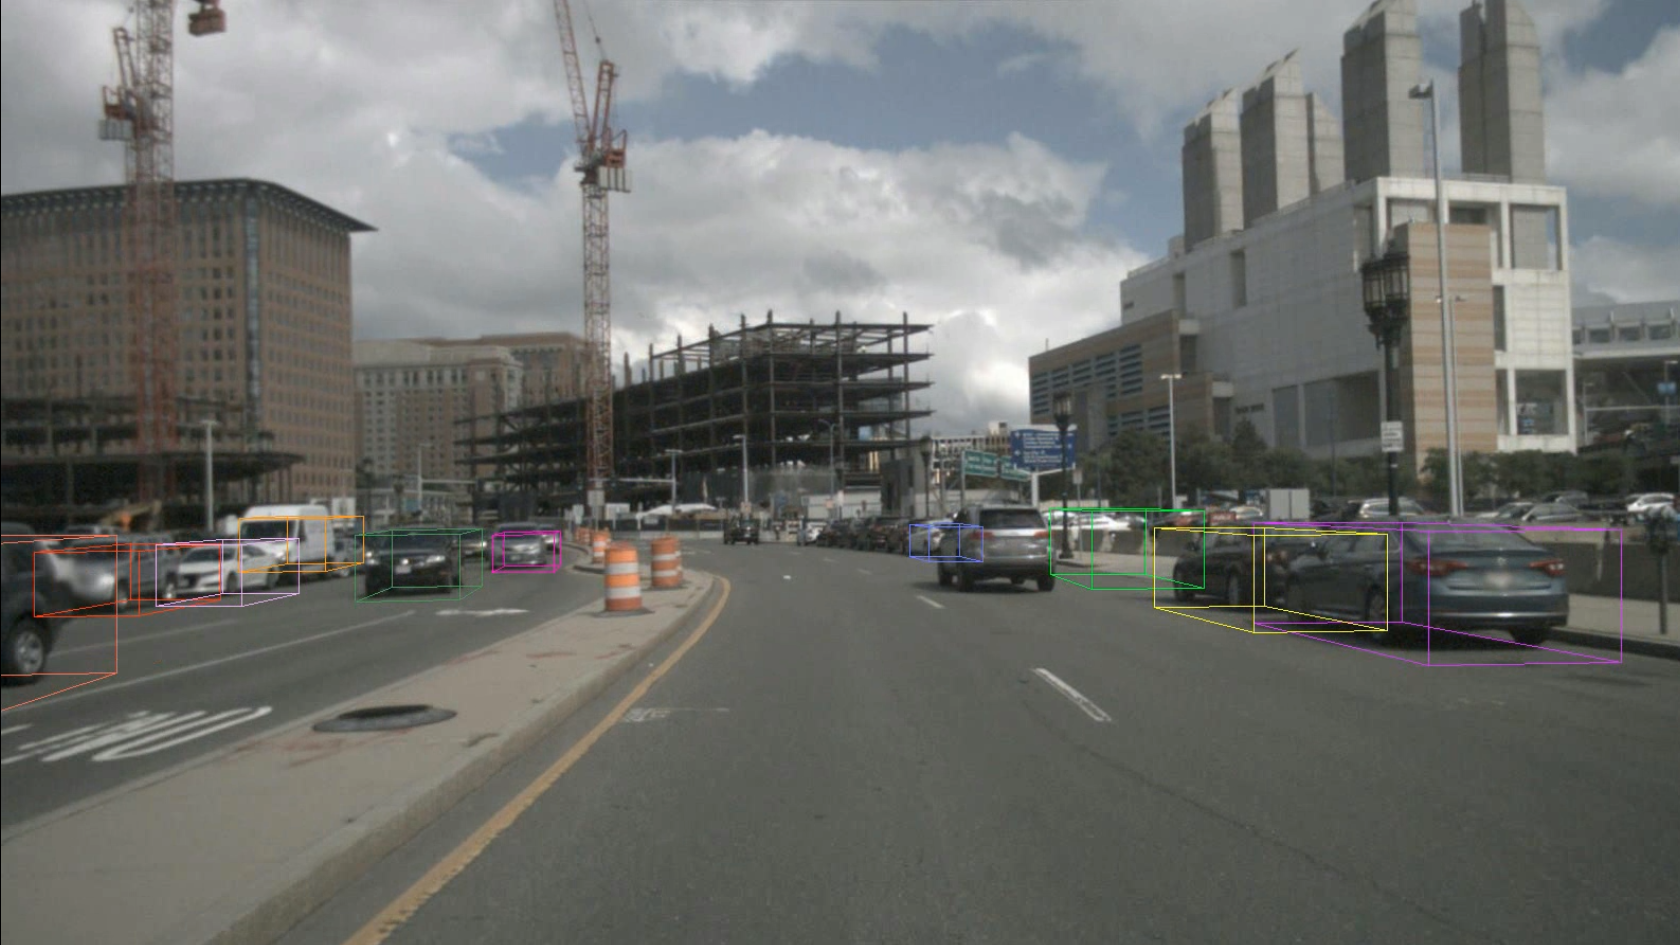
\includegraphics[width=.22\columnwidth]{fig/comp_qd/ours_01.png}} & 
        \raisebox{-0.5\height}{ 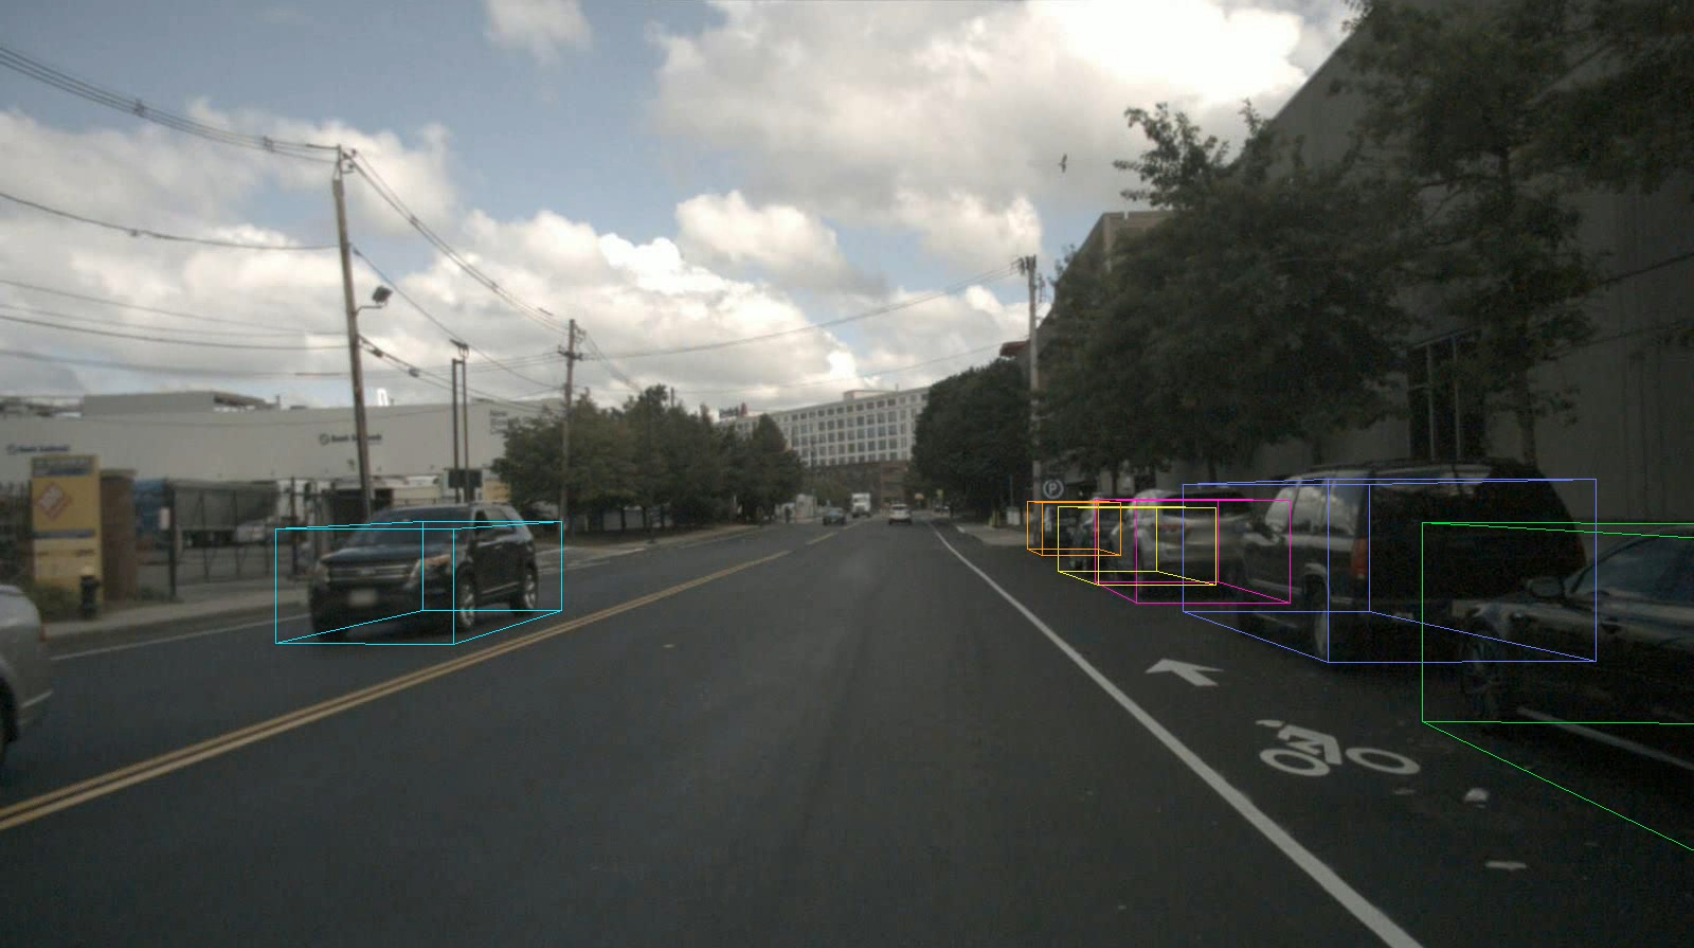
\includegraphics[width=.22\columnwidth]{fig/comp_qd/ours_11.png}} & 
        \raisebox{-0.5\height}{ 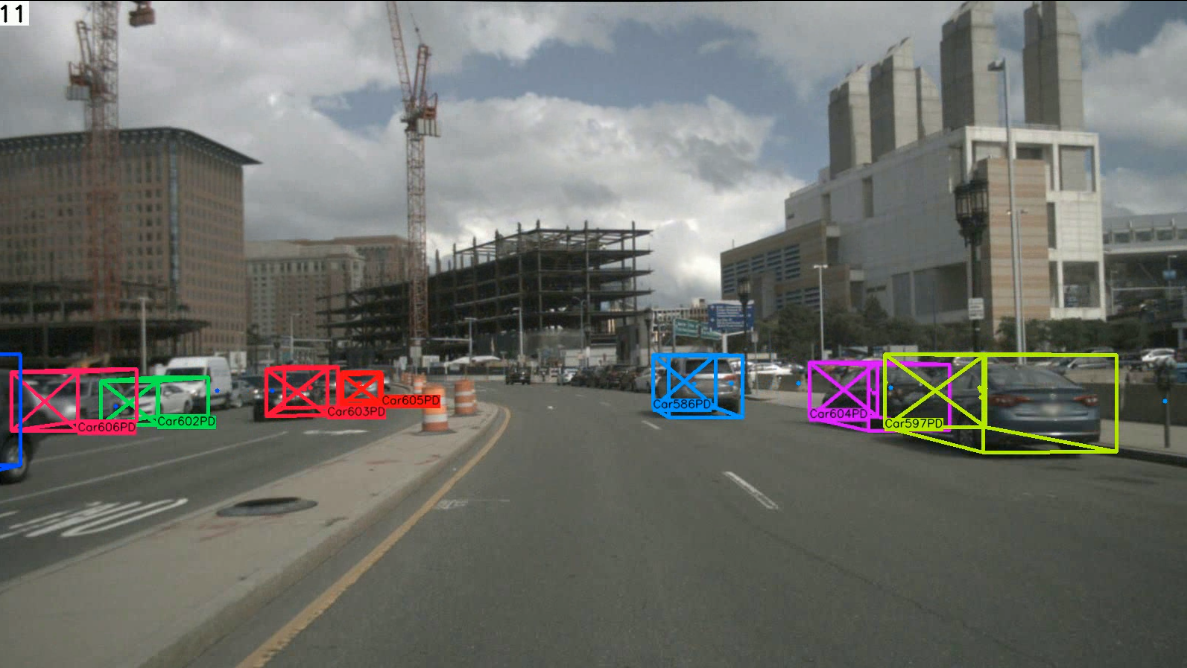
\includegraphics[width=.22\columnwidth]{fig/comp_qd/qd3dt_01.png}} & 
        \raisebox{-0.5\height}{ 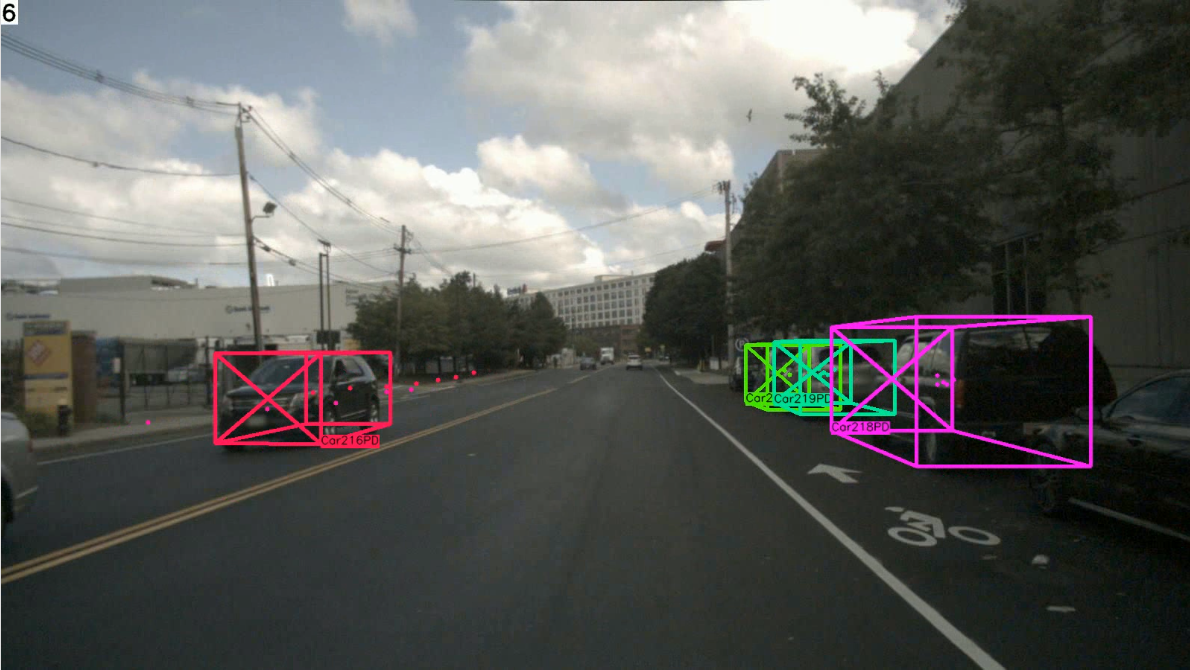
\includegraphics[width=.22\columnwidth]{fig/comp_qd/qd3dt_11.png}} \\ [0.45cm]
        
        \rotatebox[origin=c]{90}{{\footnotesize $t+1$}} &
        \raisebox{-0.5\height}{ 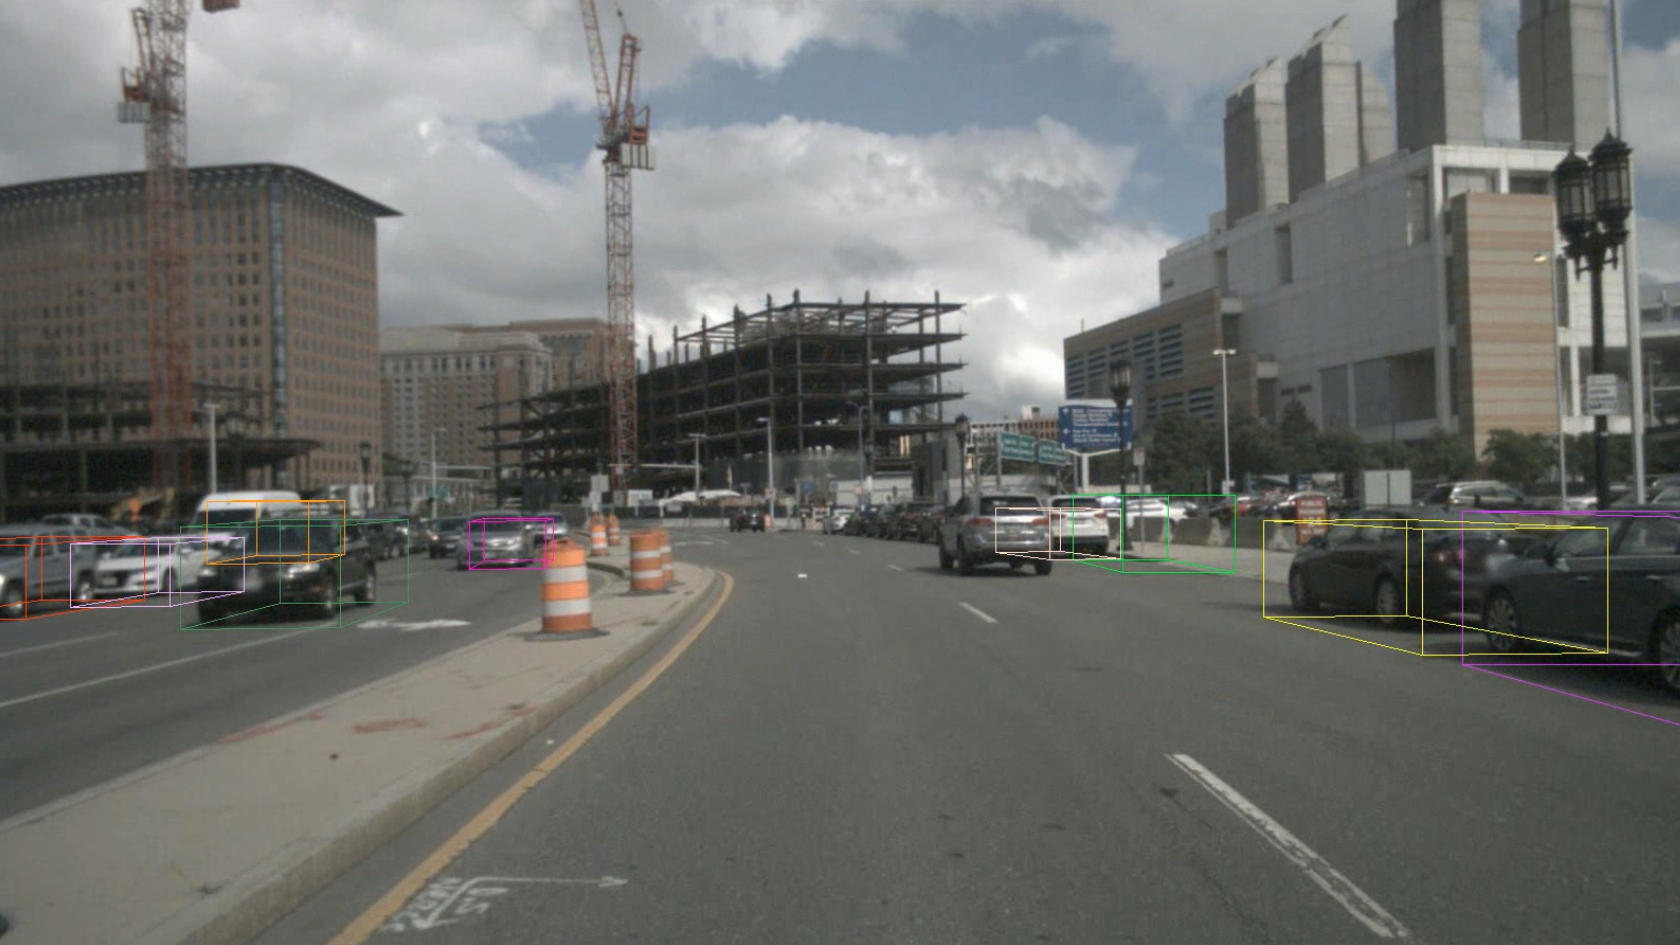
\includegraphics[width=.22\columnwidth]{fig/comp_qd/ours_02.png}} & 
        \raisebox{-0.5\height}{ 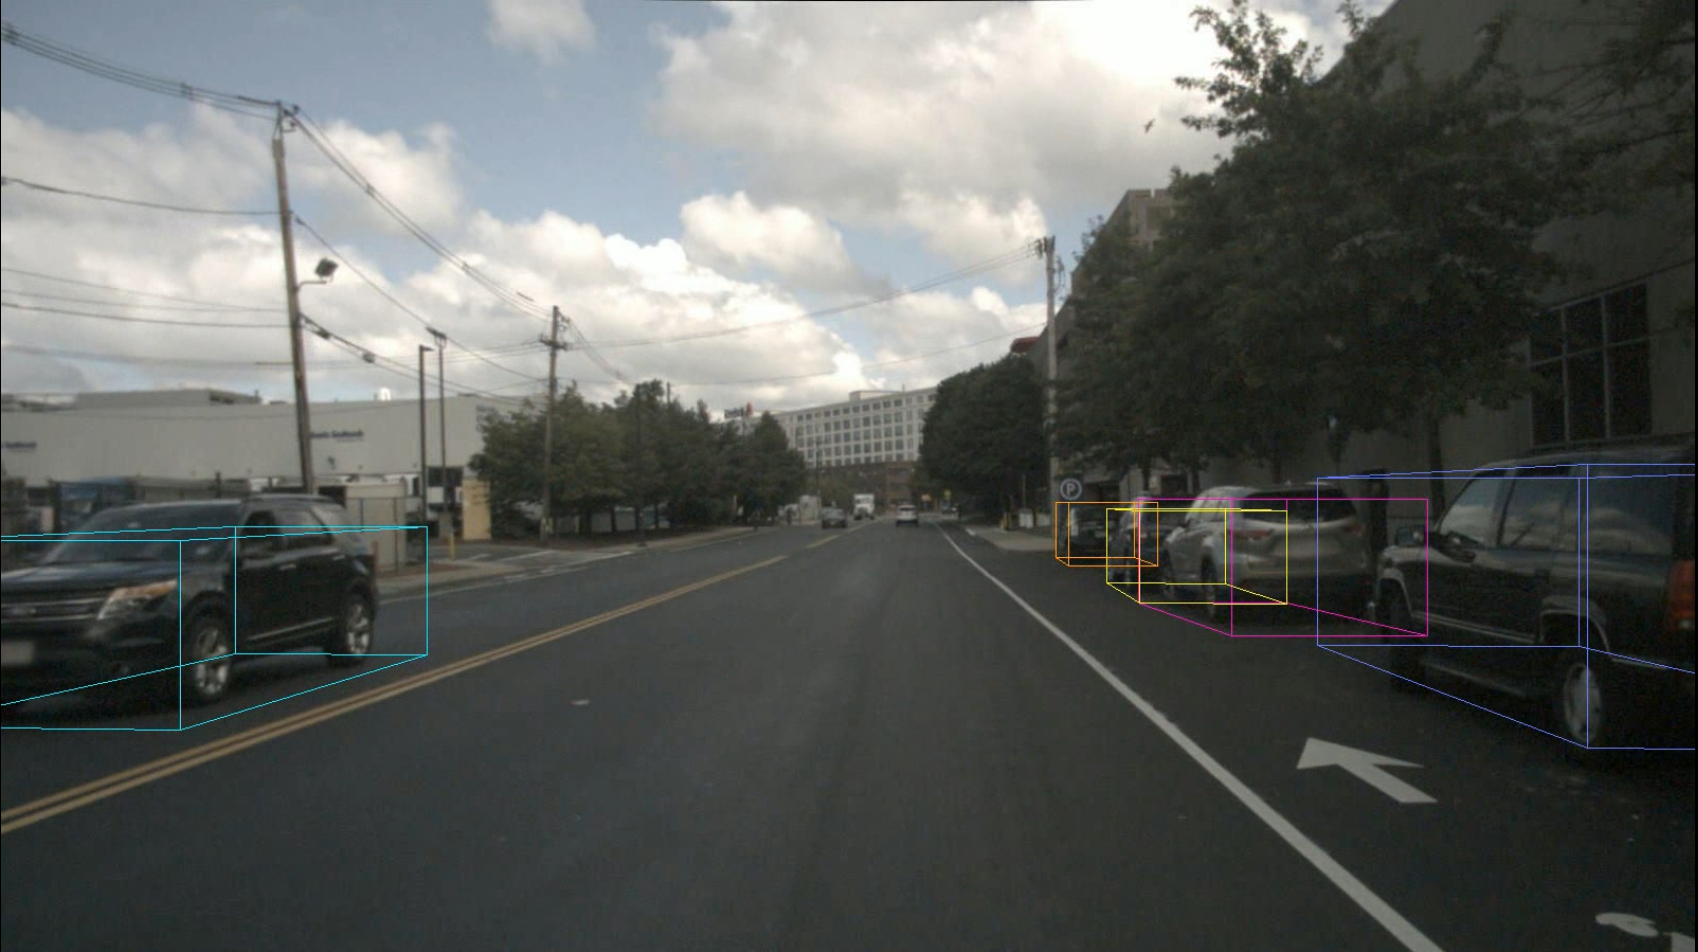
\includegraphics[width=.22\columnwidth]{fig/comp_qd/ours_12.png}} &
        \raisebox{-0.5\height}{ 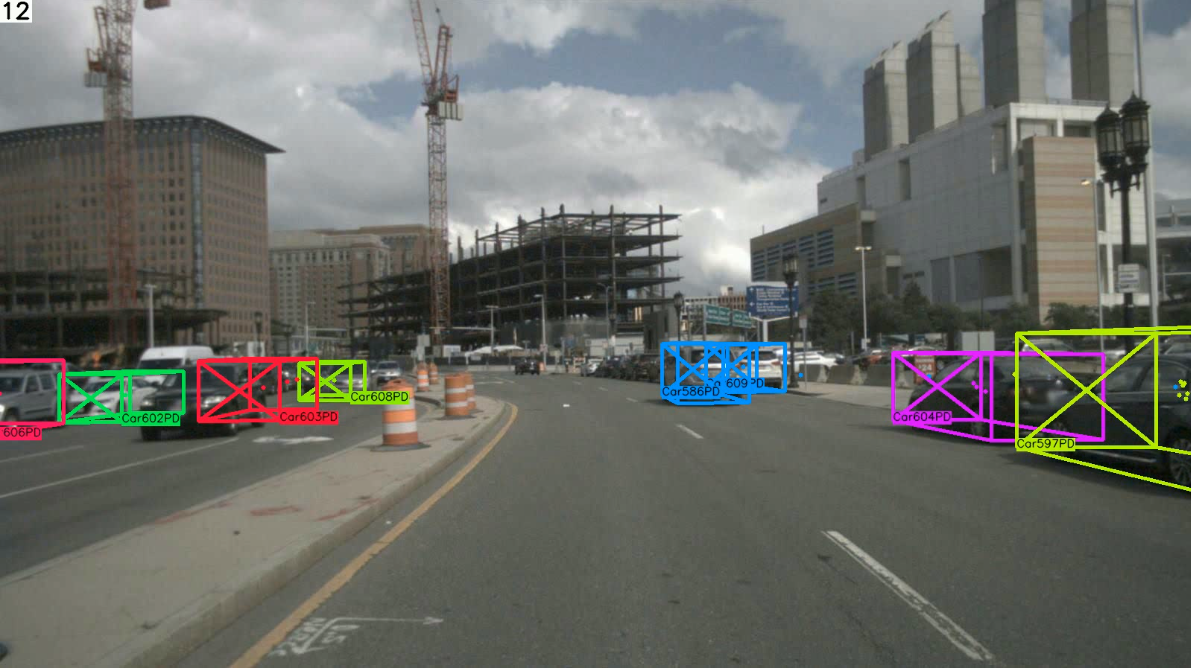
\includegraphics[width=.22\columnwidth]{fig/comp_qd/qd3dt_02.png}} & 
        \raisebox{-0.5\height}{ 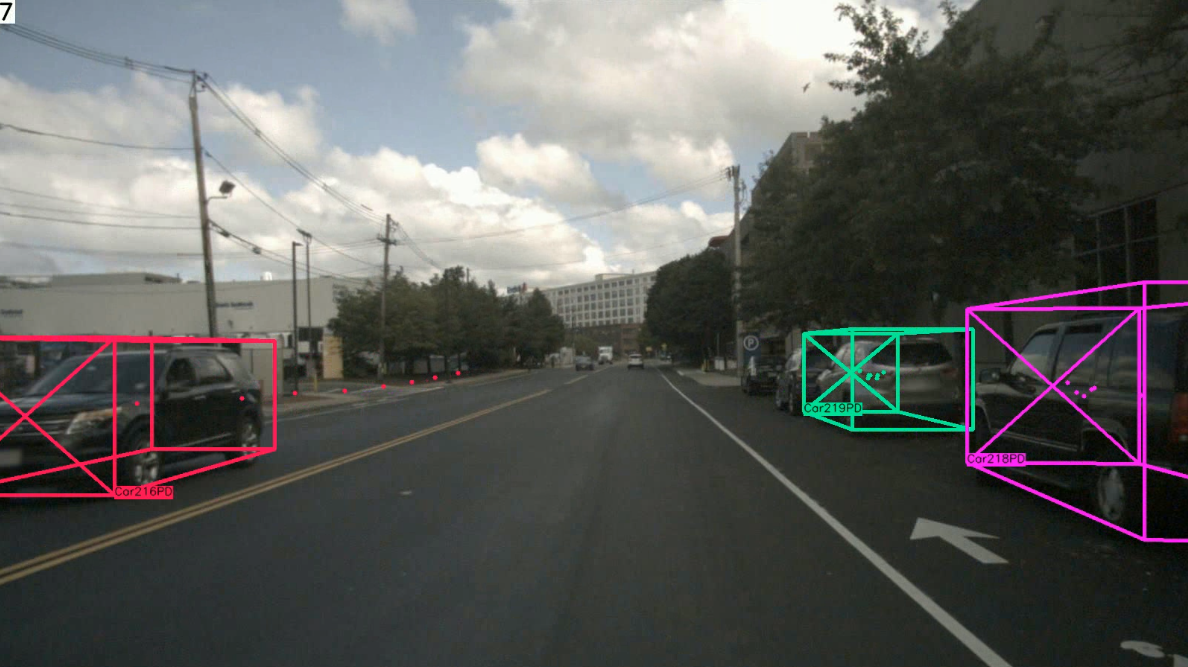
\includegraphics[width=.22\columnwidth]{fig/comp_qd/qd3dt_12.png}} \\ [0.45cm]
        & (a) & (b) & (a) & (b) \\
    \end{tabular}
    \caption{\textbf{Qualitative Comparison on Generalization.} We compare 3D bounding box outputs from QD-3DT~\cite{hu2021QD3DT} trained on waymo~\cite{sun2020scalability} and our inverse neural rendering based tracker (INR) overlayed on the respective input videos from nuscenes~\cite{caesar2020nuscenes}. The same color in consecutive frames denote same tracklet. As we see in scene (a) on the left side QD-3DT is having ID switches especially in the far range and on the sides of a frame implying dataset specific performance caps, e.g. the training dataset has been tracking annotated in a rather short range. Another finding is examplified in scene (b) on the right side were the tracker does not generalize well and is loosing a tracklet.}
    \label{tab:qd_3dt}
\end{figure}

Fig.~\ref{tab:qd_3dt} shows tracking results from our method along with results from QD-3DT. A visual, qualitative inspection illustrates that the end-to-end trained tracking method QD-3DT~\cite{sun2020scalability} still performs well on objects in the center of the scene but does not generalize well on occluded or partially visible objects. This is reflected in the scores reported in Tab. 1 of the main manuscript.





\subsection{Additional Results on nuScenes} Although the nuScenes~\cite{caesar2020nuscenes} dataset consists of sensor data from 6 cameras, 5 radars, and 1 lidar, we tackle monocular camera-based 3D object tracking in this work. As such, we only use the data collected from the 6 cameras. The dataset comprises 1000 scenes, with each scene being 20s long. The test set contains 150 scenes. Each of these scenes is selected to be \textit{interesting}, which include scenes with high traffic density (e.g., intersections, construction sites), rare classes (e.g. ambulances, animals), potentially dangerous traffic situations (e.g., jaywalkers, incorrect behavior), maneuvers (e.g., lane change, turning, stopping) and situations that may be difficult for an Autonomous Vehicle. Additional results of our method on the nuScenes dataset are listed in Fig.~\ref{fig:additional_nuScenes_results}. We note that the colors of the cars are matched quite accurately.
Moreover, the shapes of the cars get reconstructed as well. In turn, we can see that the tracking quality is high as visualized by bounding boxes. Note that the color of bounding boxes marks the same instance in consecutive frames. 
% \todo{describe the results.}

\subsection{Additional Results on Waymo Open Dataset} The Waymo Open Dataset~\cite{sun2020scalability} consists of 1150 scenes that each span 20s. Again, since we tackle monocular tracking, we only use the data from the 5 camera sensors. The dataset was collected by driving in Phoenix AZ, Mountain View CA, and San Francisco CA across daytime, nighttime, and dawn lighting conditions. Additional results of our method on the Waymo Open dataset are given in Figure \ref{fig:additional_waymo_results}. We find that our method generalizes effectively to this dataset. The colors of the cars are matched quite accurately, as shown in Figure \ref{fig:additional_waymo_results}. Moreover, the shapes of the cars get reconstructed as well. As such, again, tracking quality is high as visualized by bounding boxes. Note that the color of bounding boxes marks the same instance in consecutive frames. 
% ~\todo{Actually describe results.}
\newpage
\begin{figure*}[h!]
	\vspace{-5pt}
	\centering
	\resizebox{0.98\linewidth}{!}{
	\renewcommand{\arraystretch}{0.5}
	\begin{tabular}{@{}c@{\hskip 0.05cm}c@{\hskip 0.05cm}c@{\hskip 0.05cm}c@{\hskip 0.05cm}c@{\hskip 0.05cm}c@{}}
		\centering
            &
		{\huge Input $t_0$}&
		{\huge Tracked $t_0$}&
		{\huge Tracked $t_1$}&
		{\huge Tracked $t_2$}&
		{\huge Tracked $t_3$}\\

            \rotatebox[origin=c]{90}{{\Large	  Crossing 1}}&
		 \raisebox{-0.5\height}{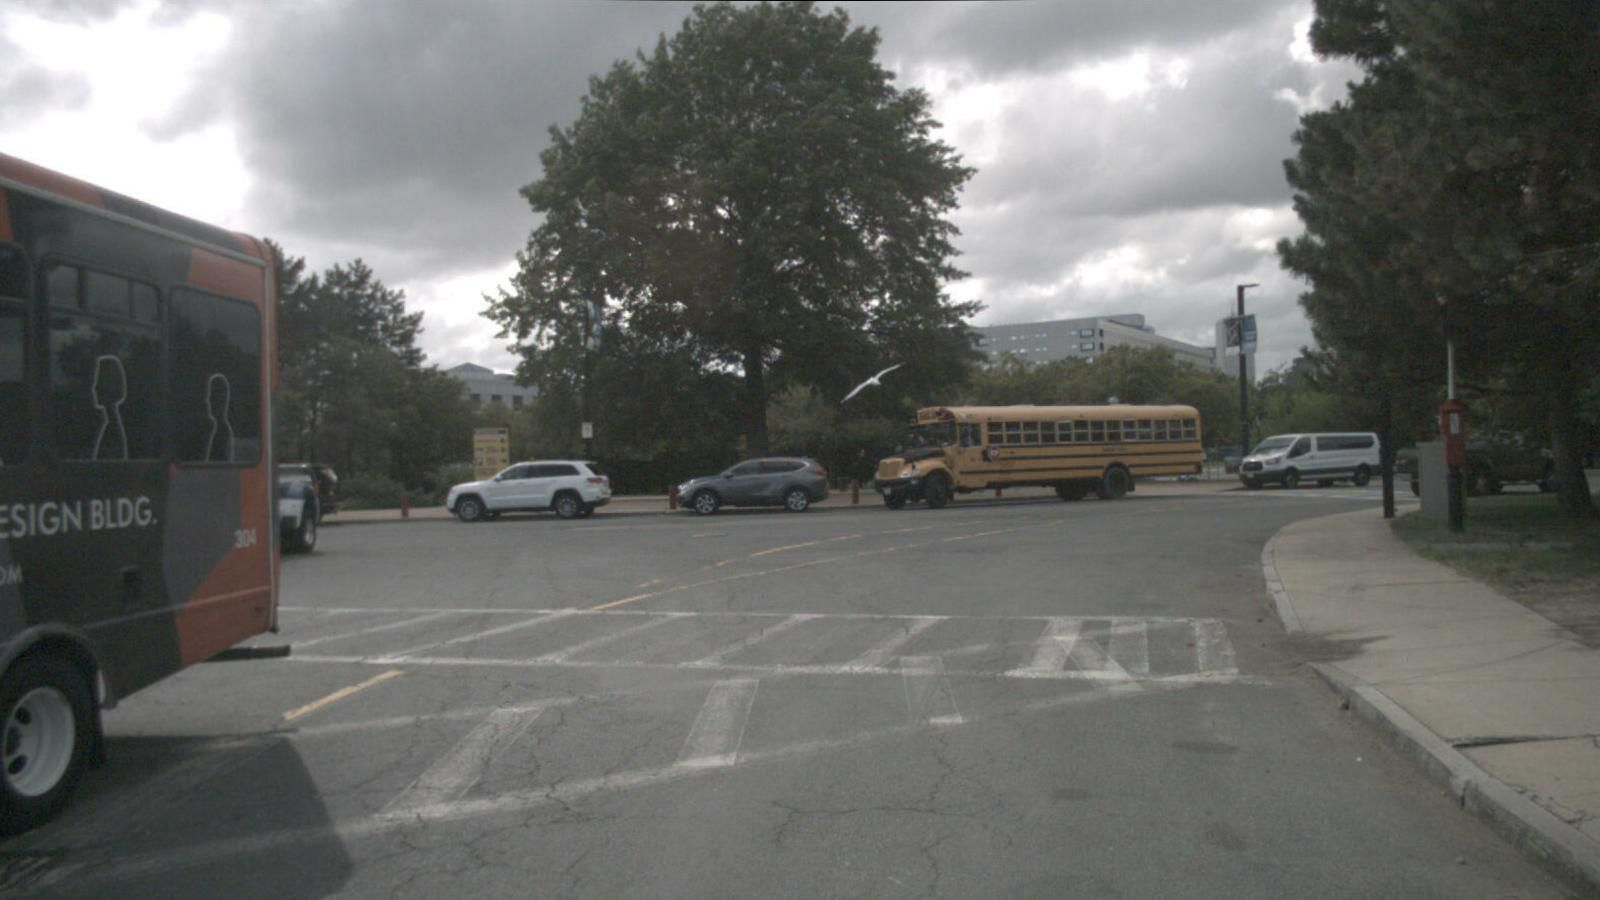
\includegraphics[width=.38\columnwidth, trim={0cm 0cm 0cm 0cm},clip]{fig/additional_nuscenes_results/scene1/26_gt.png}}&
		 \raisebox{-0.5\height}{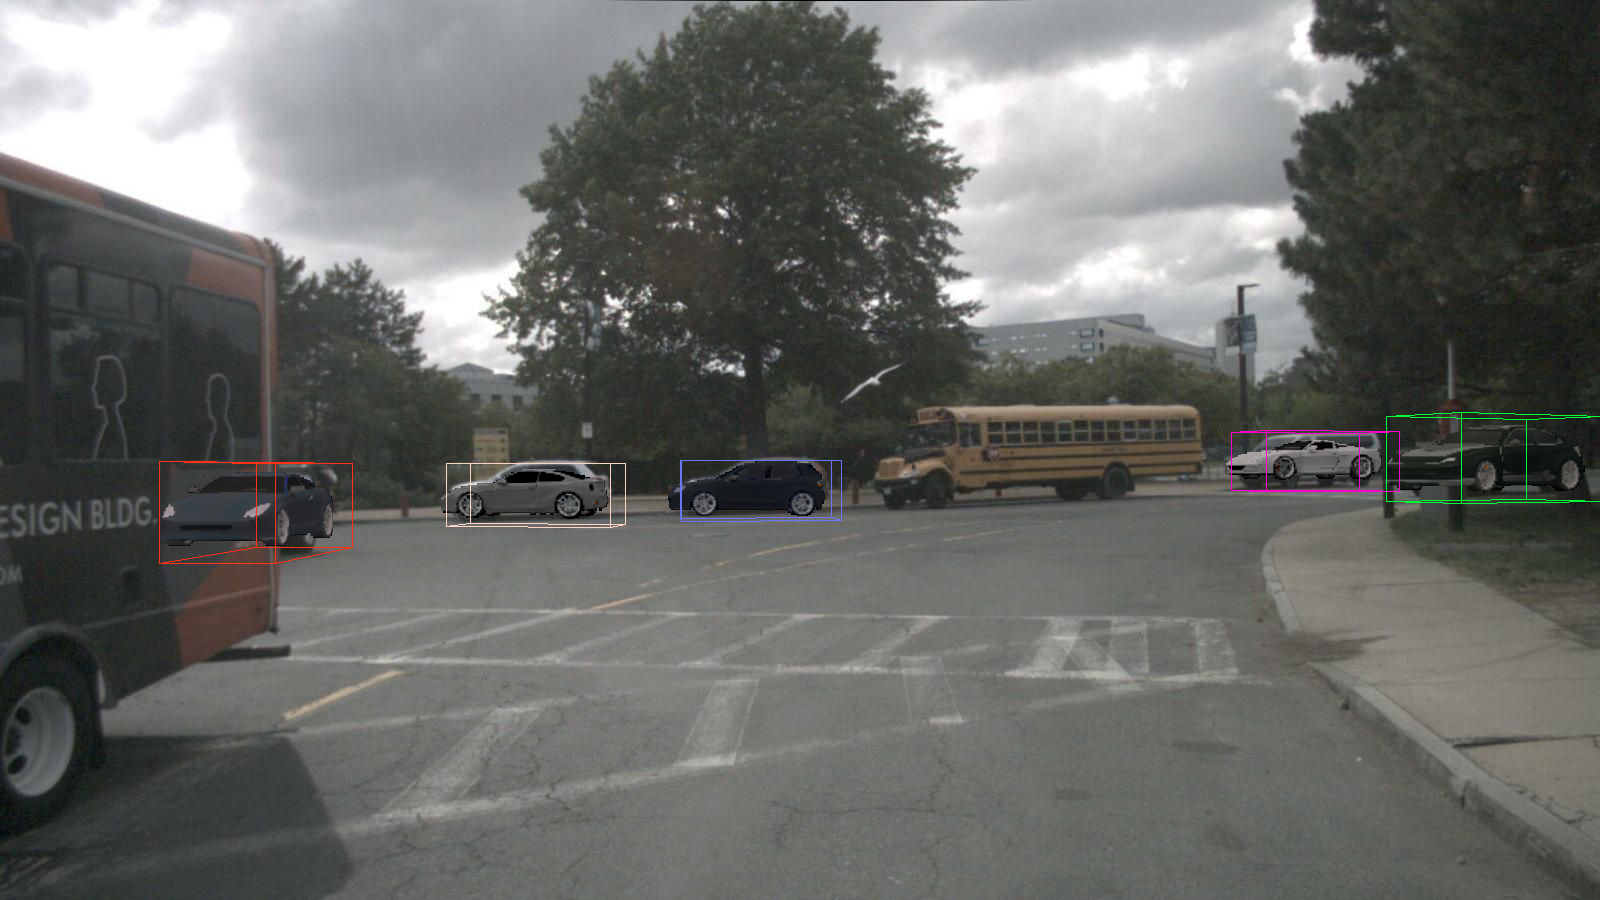
\includegraphics[width=.38\columnwidth, trim={0cm 0cm 0cm 0cm},clip]{fig/additional_nuscenes_results/scene1/26_bbox.png}}&
		 \raisebox{-0.5\height}{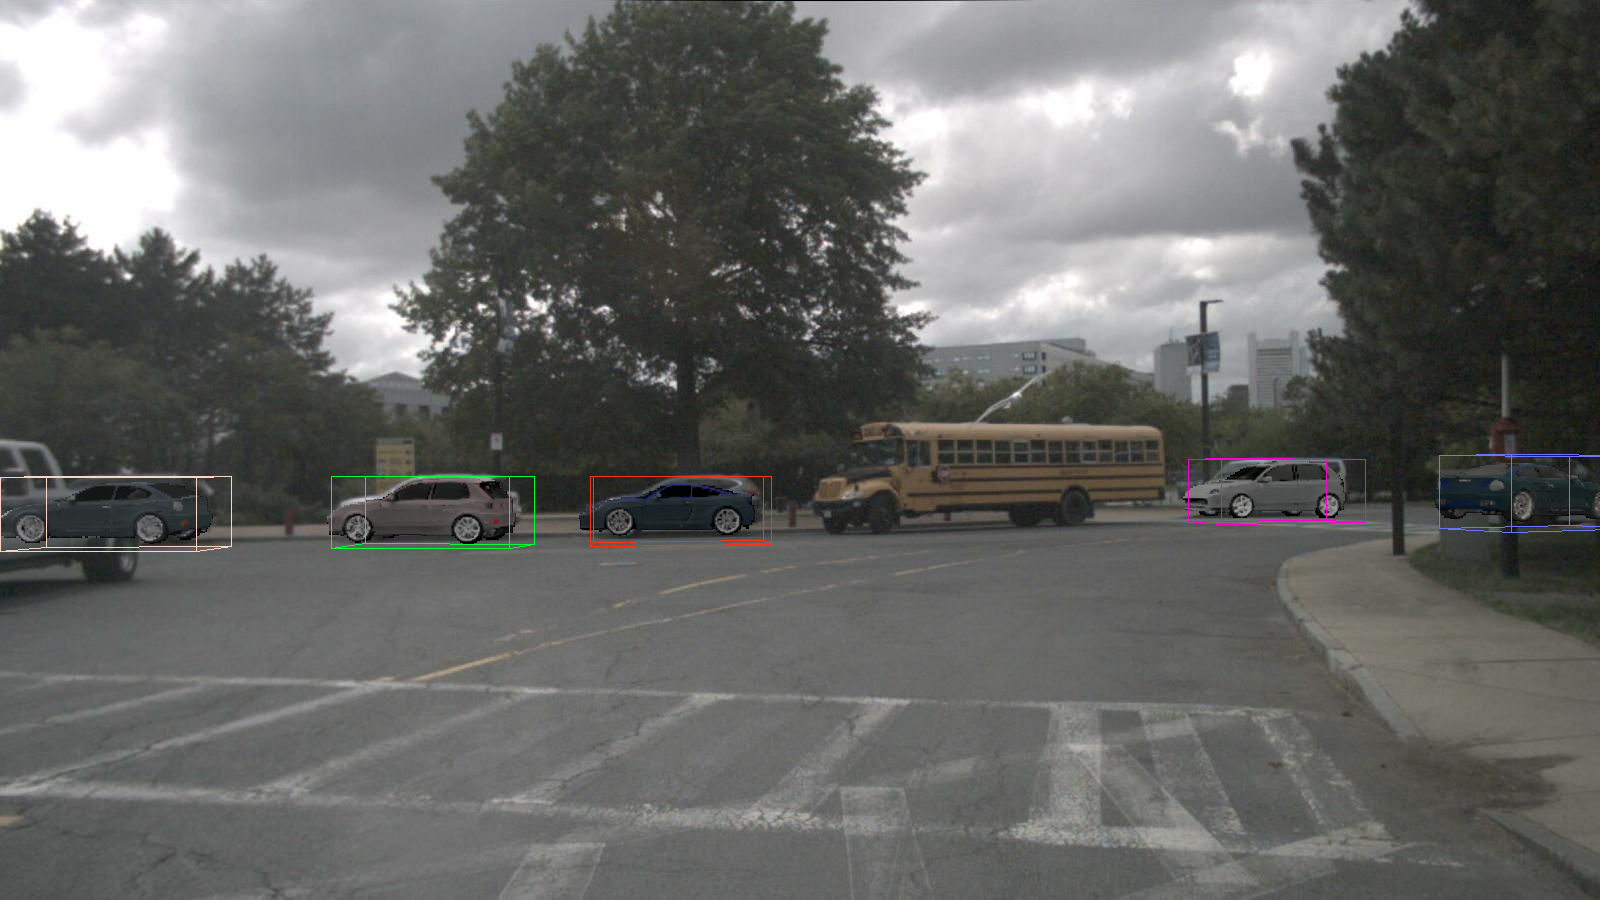
\includegraphics[width=.38\columnwidth, trim={0cm 0cm 0cm 0cm},clip]{fig/additional_nuscenes_results/scene1/27_bbox.png}}&
		 \raisebox{-0.5\height}{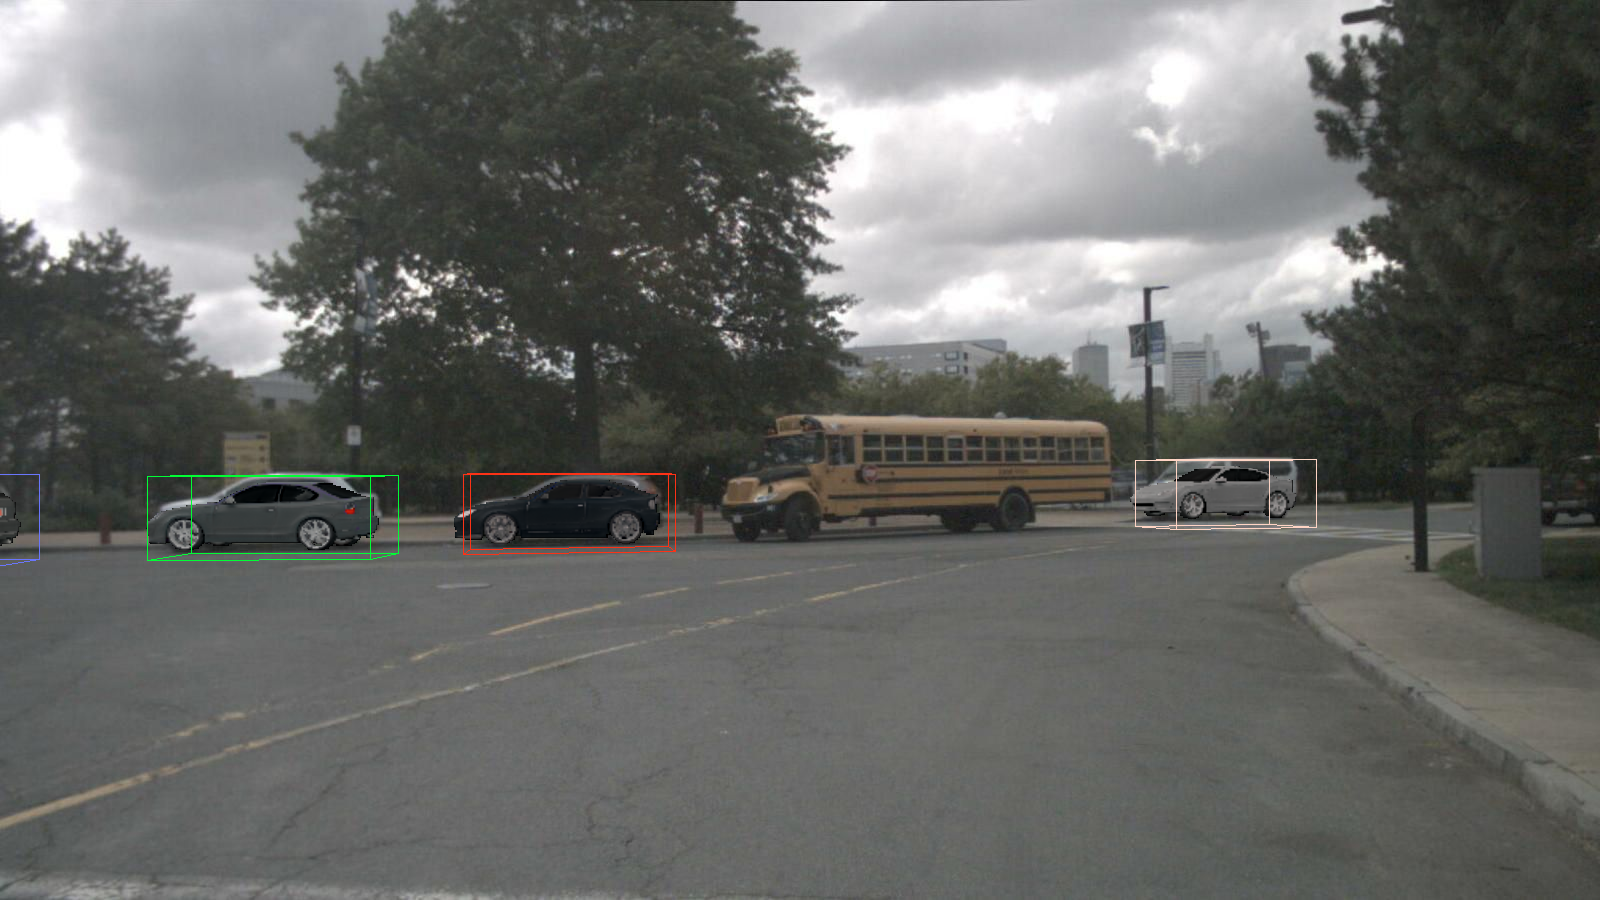
\includegraphics[width=.38\columnwidth, trim={0cm 0cm 0cm 0cm},clip]{fig/additional_nuscenes_results/scene1/28_bbox.png}}&
		 \raisebox{-0.5\height}{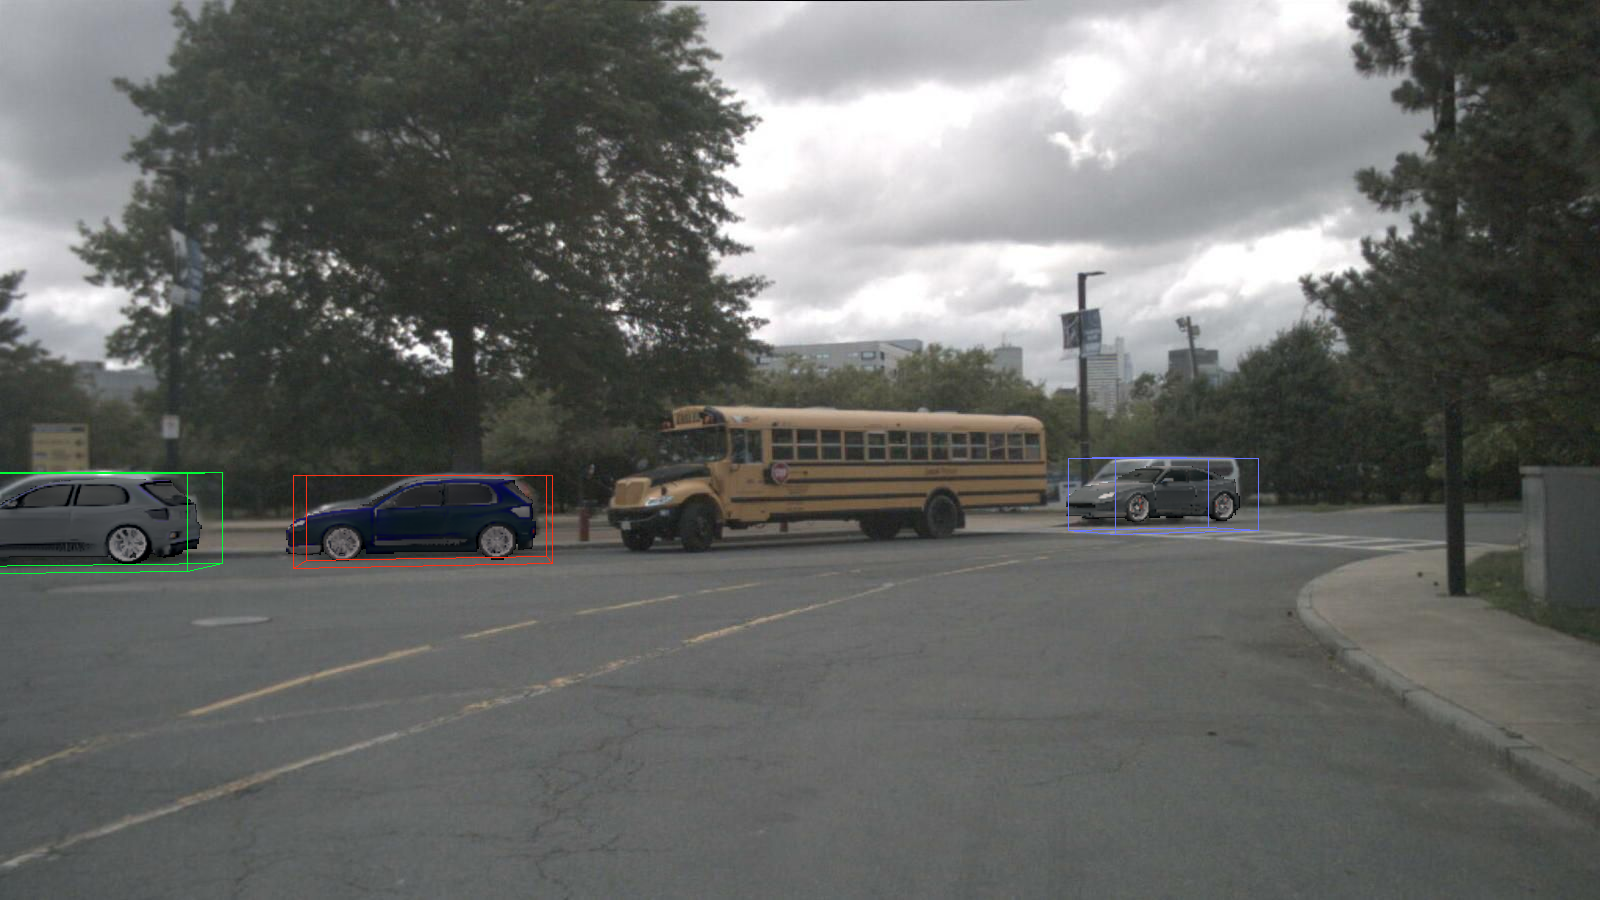
\includegraphics[width=.38\columnwidth, trim={0cm 0cm 0cm 0cm},clip]{fig/additional_nuscenes_results/scene1/29_bbox.png}}\\[1.5cm]
  
		\rotatebox[origin=c]{90}{{\Large	 Traffic}}&
		\raisebox{-0.5\height}{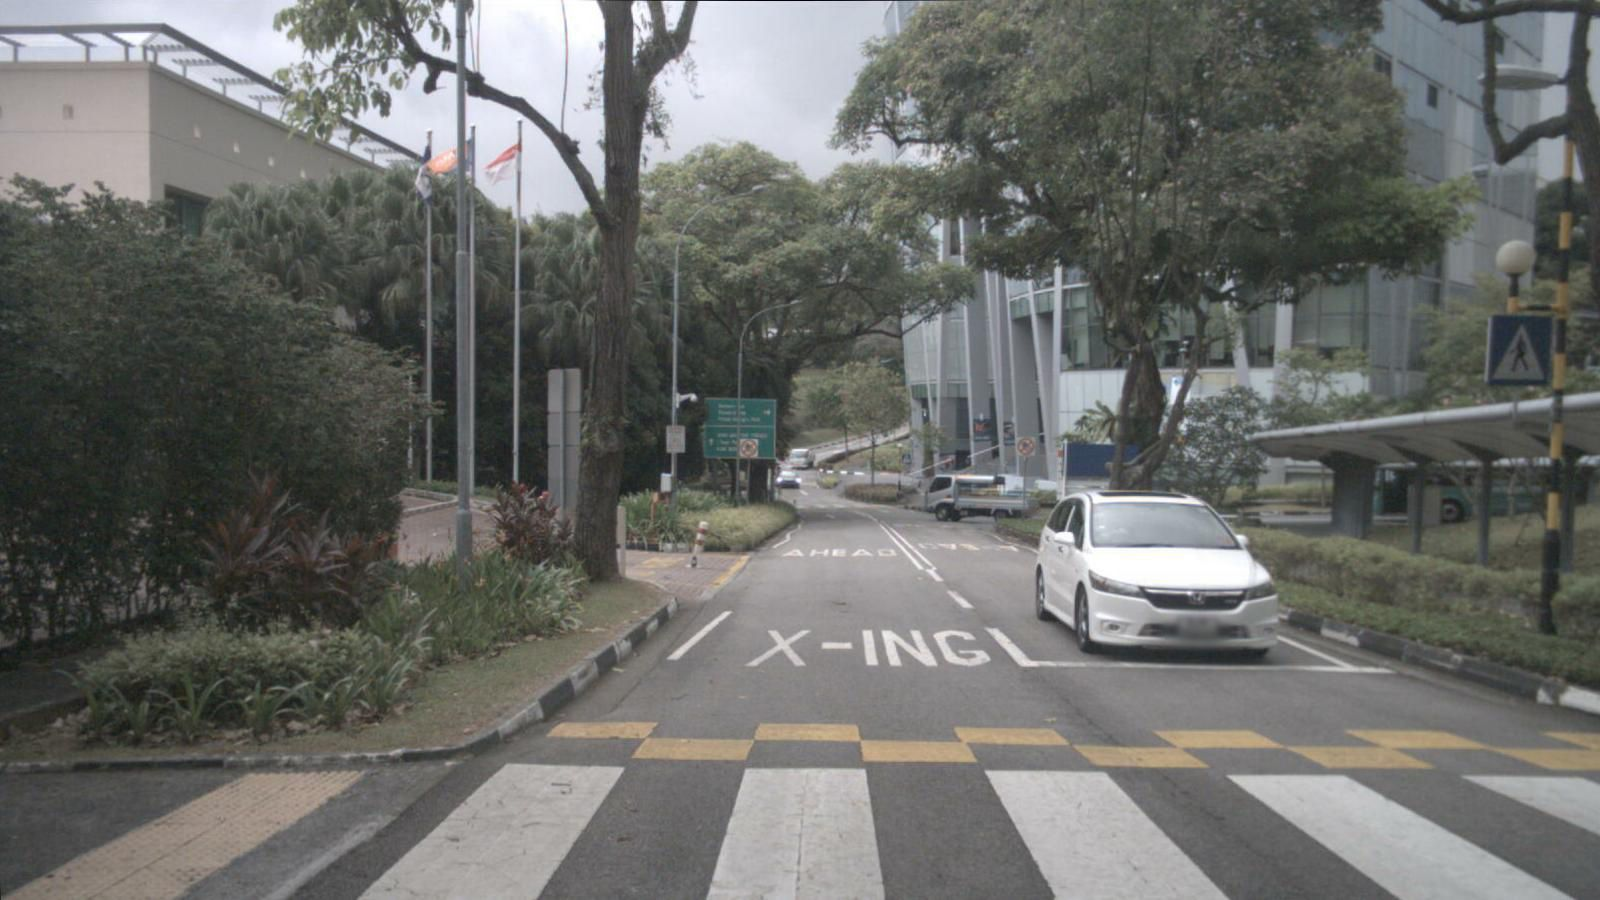
\includegraphics[width=.38\columnwidth, trim={0cm 0cm 0cm 0cm},clip]{fig/additional_nuscenes_results/scene13/gt_img.png}}&
		\raisebox{-0.5\height}{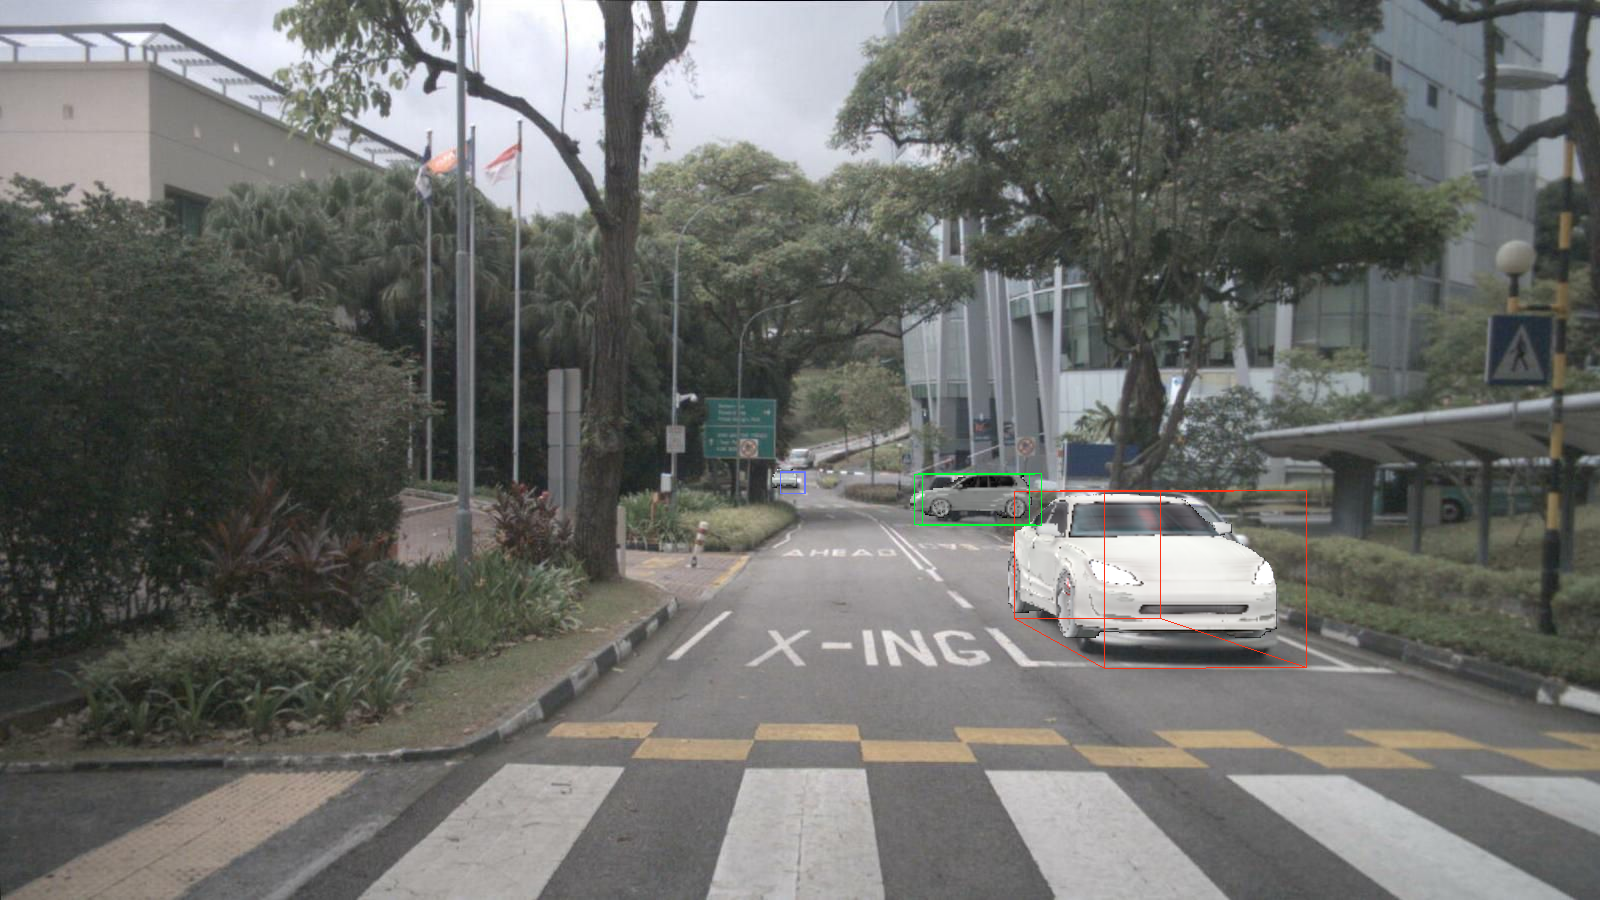
\includegraphics[width=.38\columnwidth, trim={0cm 0cm 0cm 0cm},clip]{fig/additional_nuscenes_results/scene13/23.png}} &
		\raisebox{-0.5\height}{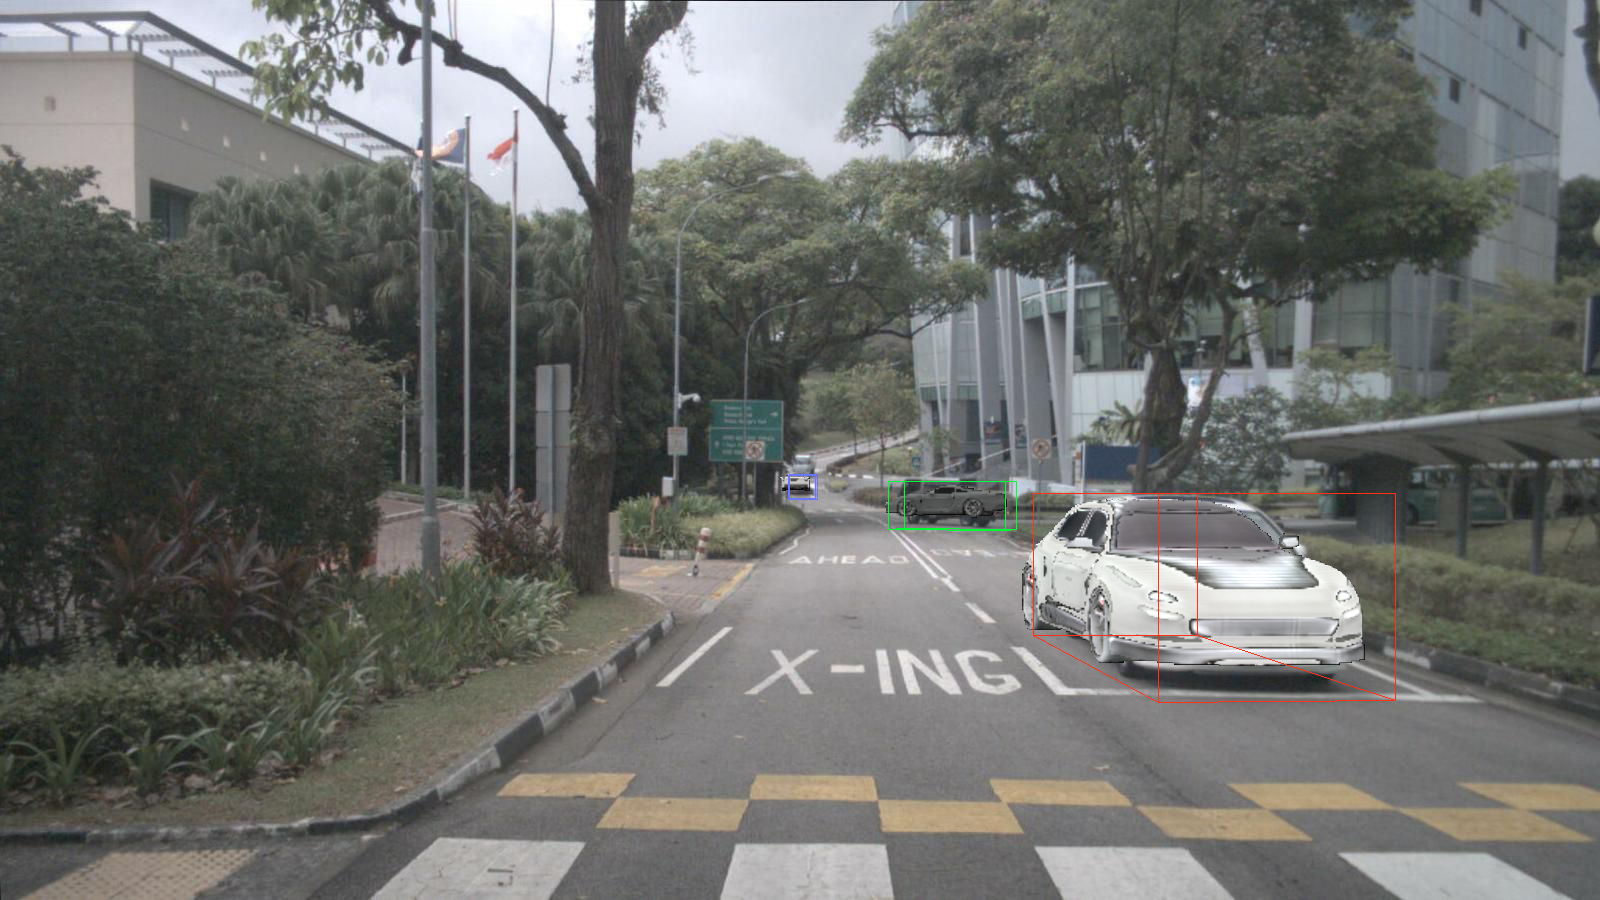
\includegraphics[width=.38\columnwidth, trim={0cm 0cm 0cm 0cm},clip]{fig/additional_nuscenes_results/scene13/24.png}}&
		\raisebox{-0.5\height}{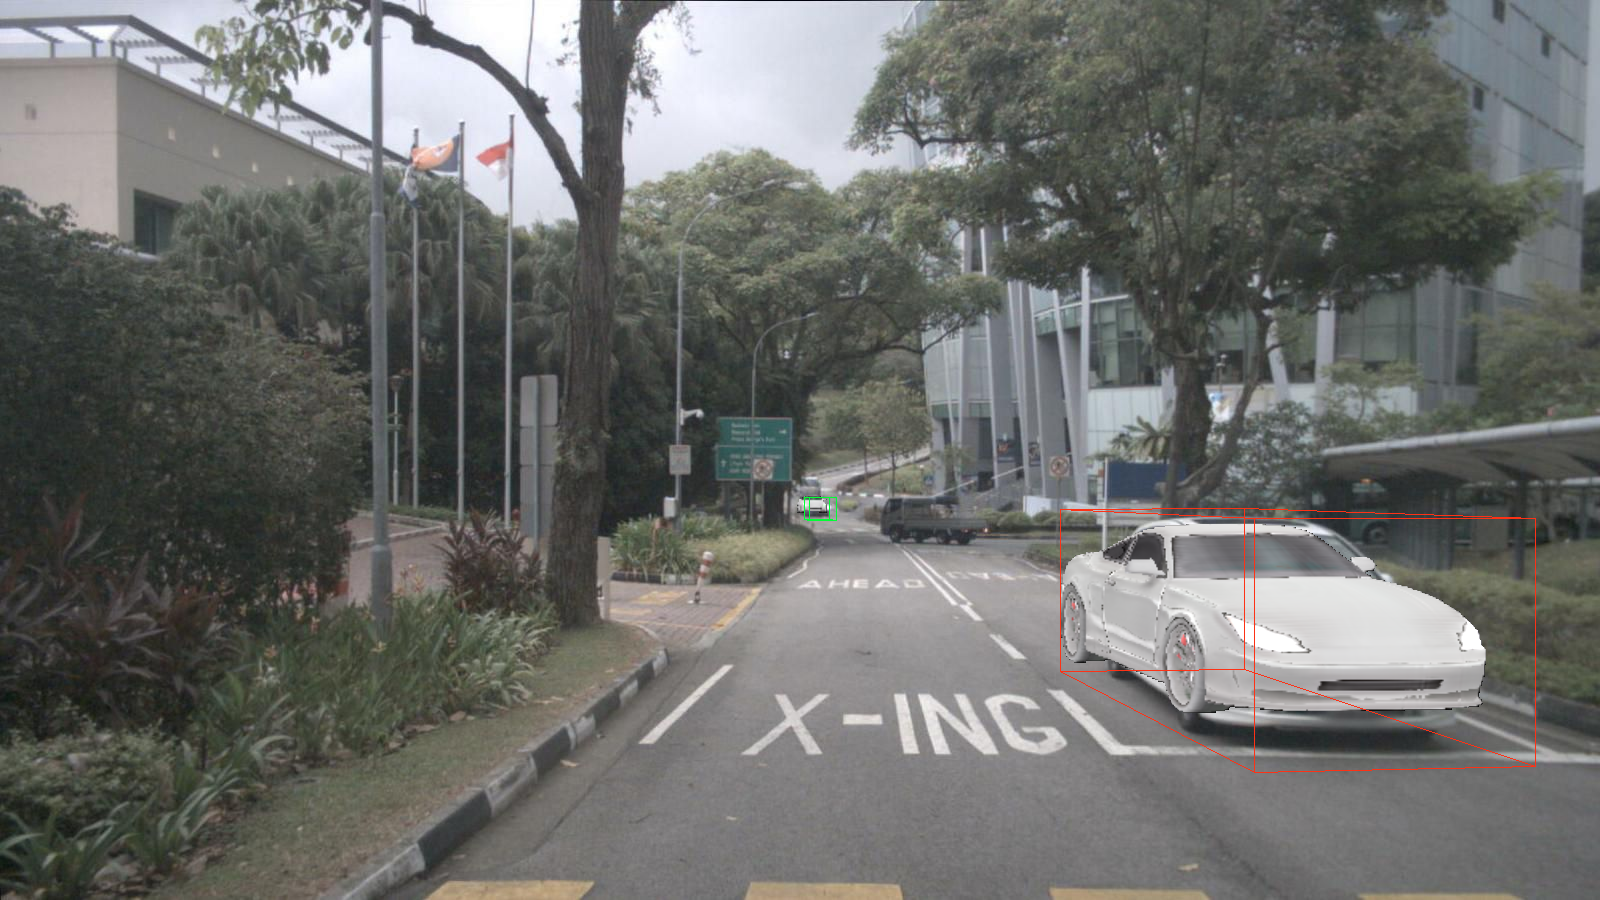
\includegraphics[width=.38\columnwidth, trim={0cm 0cm 0cm 0cm},clip]{fig/additional_nuscenes_results/scene13/25.png}}&
		\raisebox{-0.5\height}{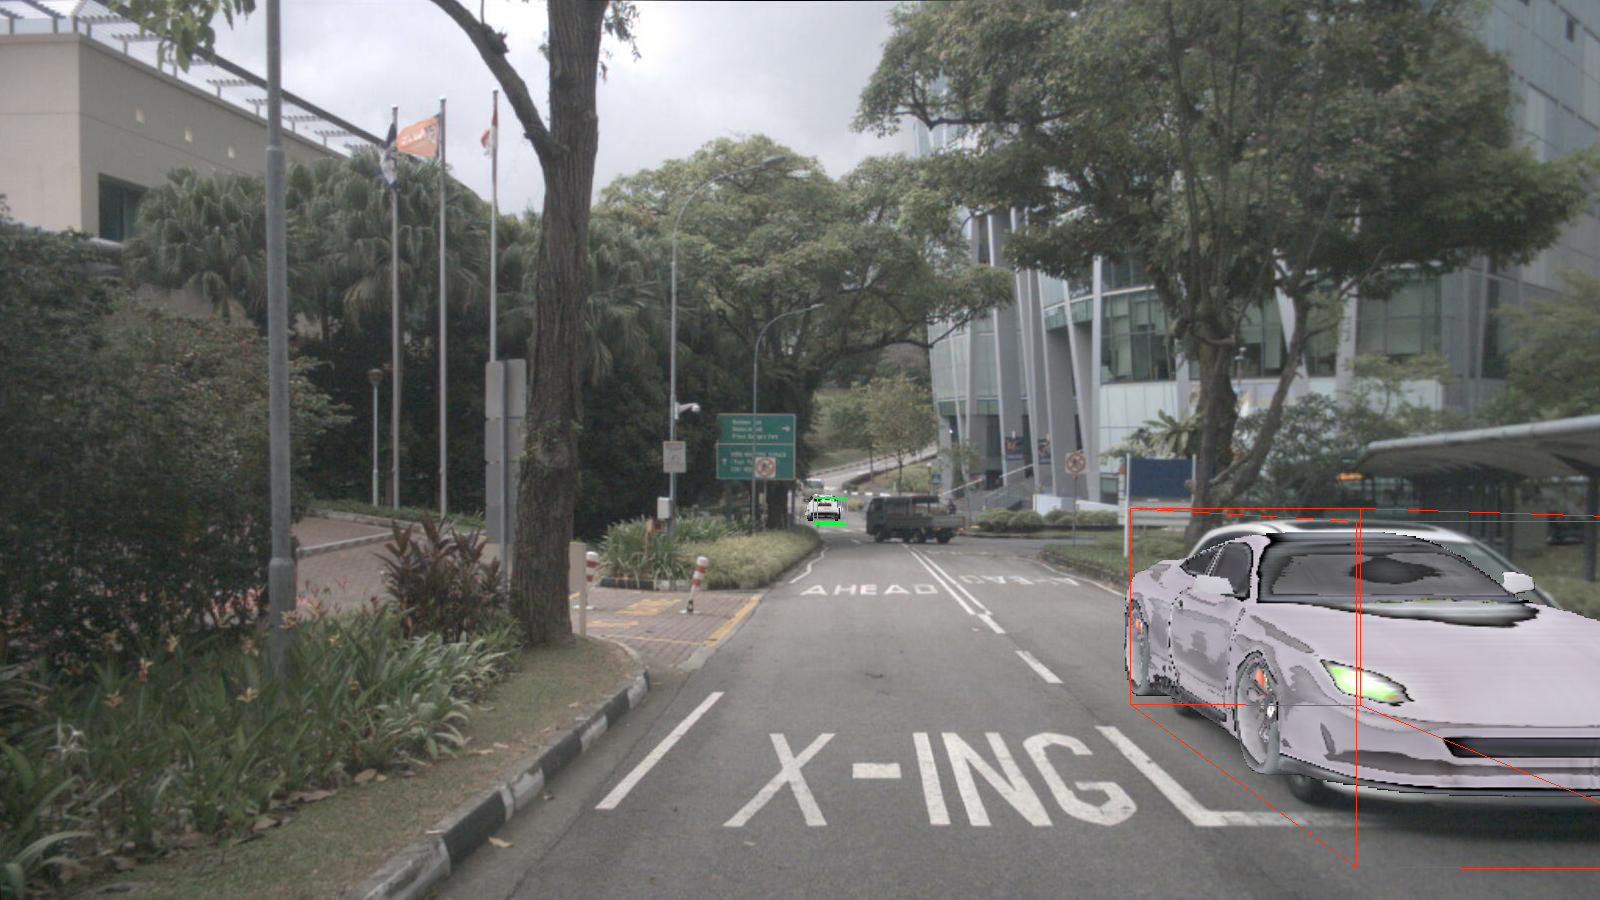
\includegraphics[width=.38\columnwidth, trim={0cm 0cm 0cm 0cm},clip]{fig/additional_nuscenes_results/scene13/26.png}}\\[1.5cm]
  
            \rotatebox[origin=c]{90}{{\Large	Urban 1}}&
  		\raisebox{-0.5\height}{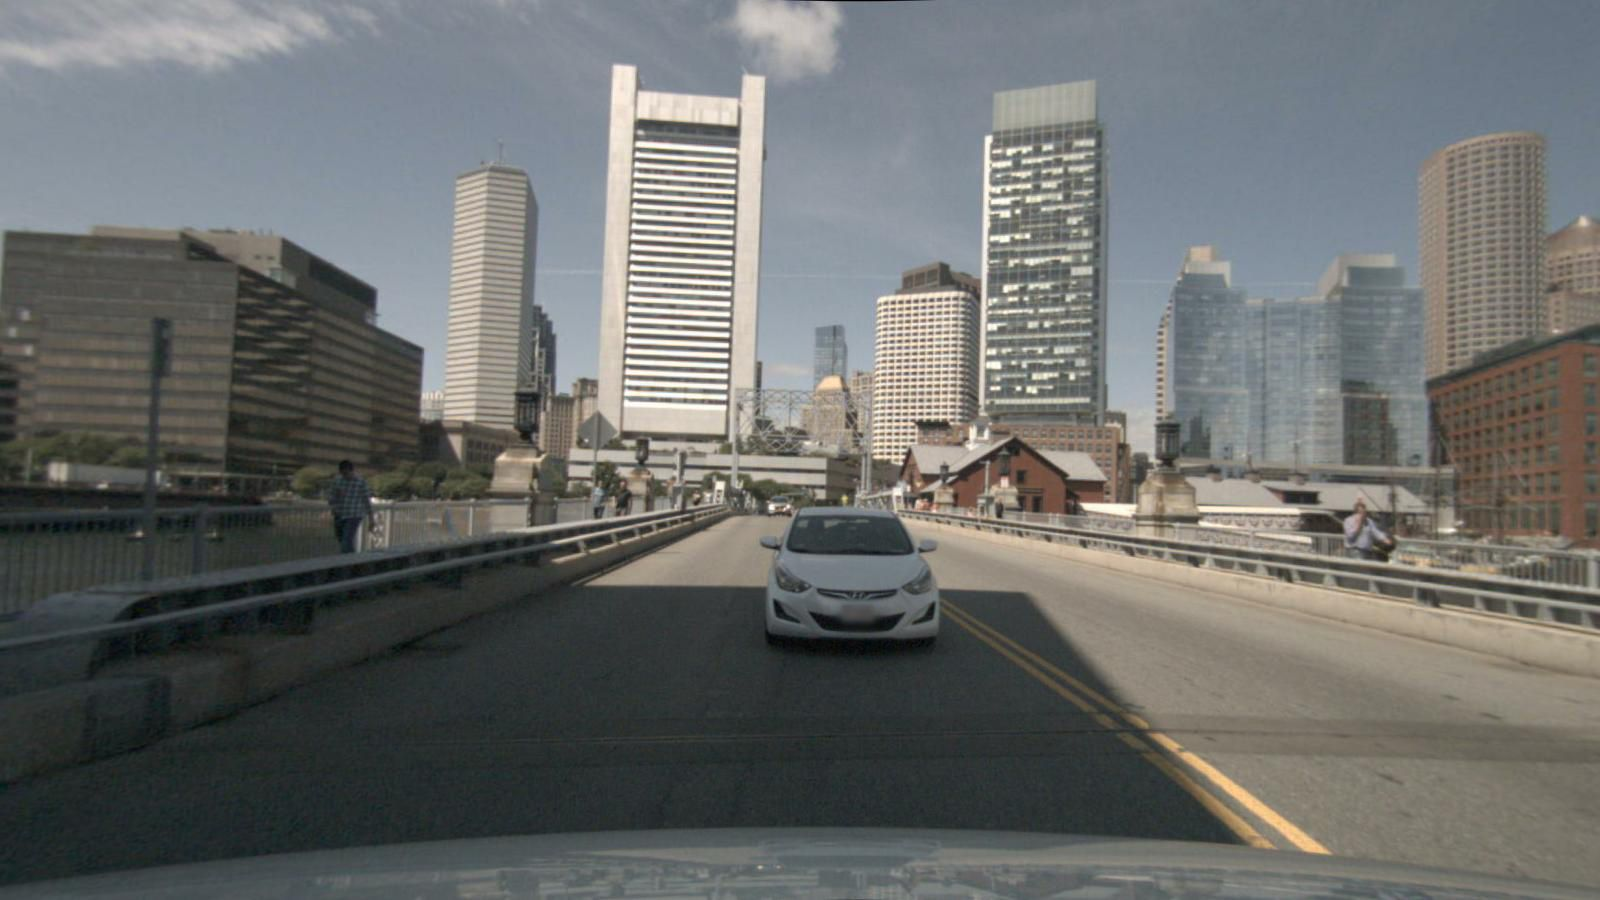
\includegraphics[width=.38\columnwidth, trim={0cm 0cm 0cm 0cm},clip]{fig/additional_nuscenes_results/scene12/gt.png}}&
		\raisebox{-0.5\height}{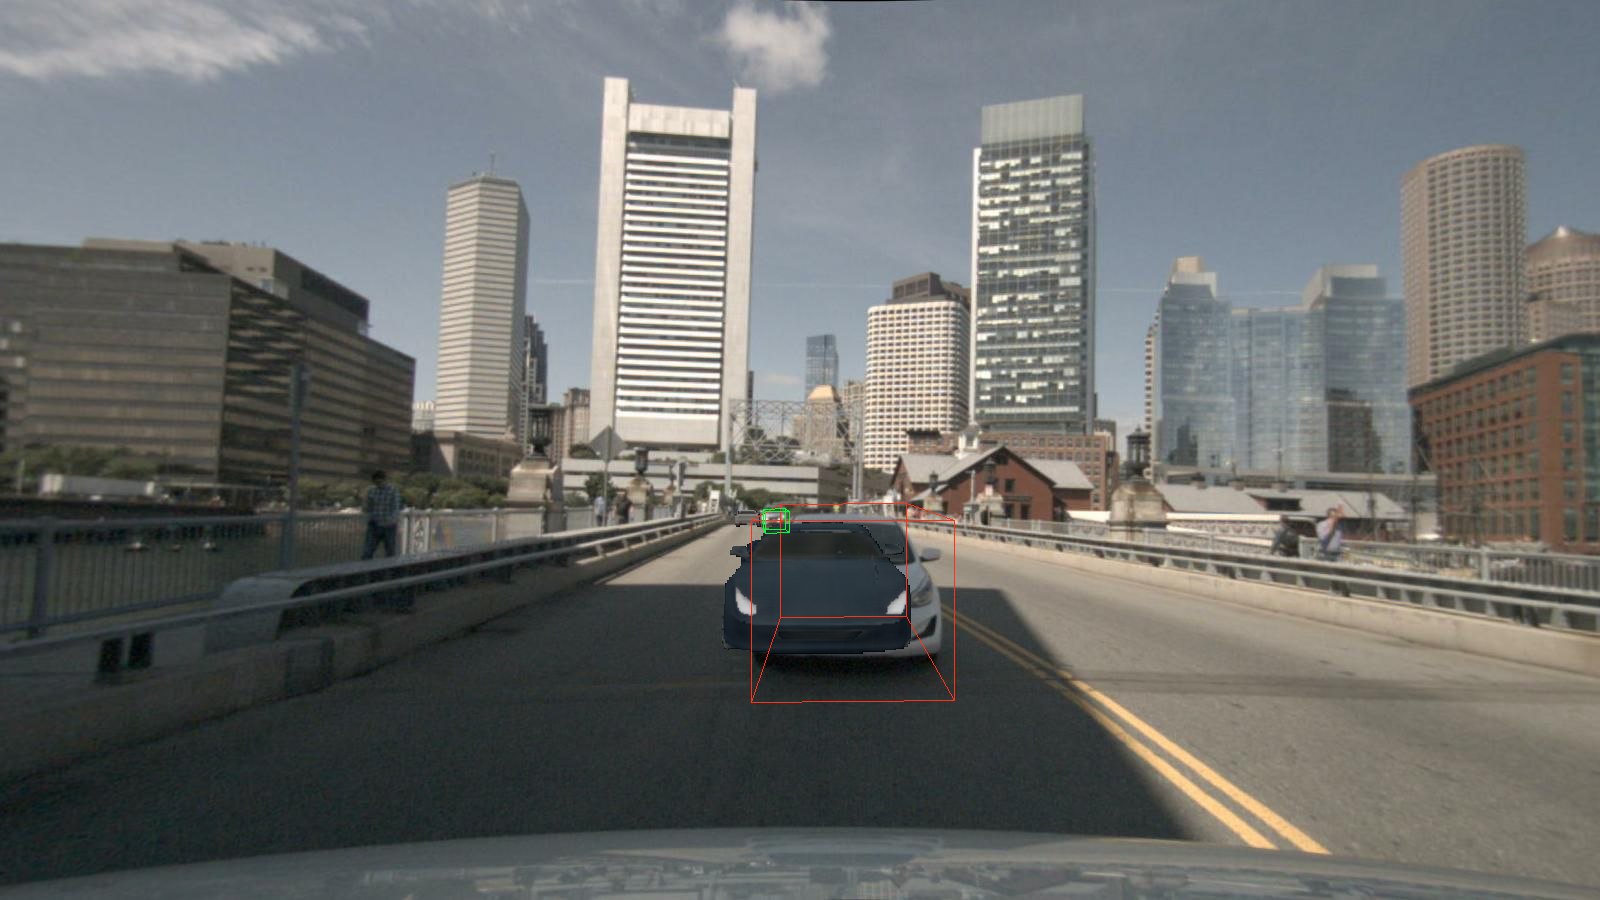
\includegraphics[width=.38\columnwidth, trim={0cm 0cm 0cm 0cm},clip]{fig/additional_nuscenes_results/scene12/21.png}}&
		\raisebox{-0.5\height}{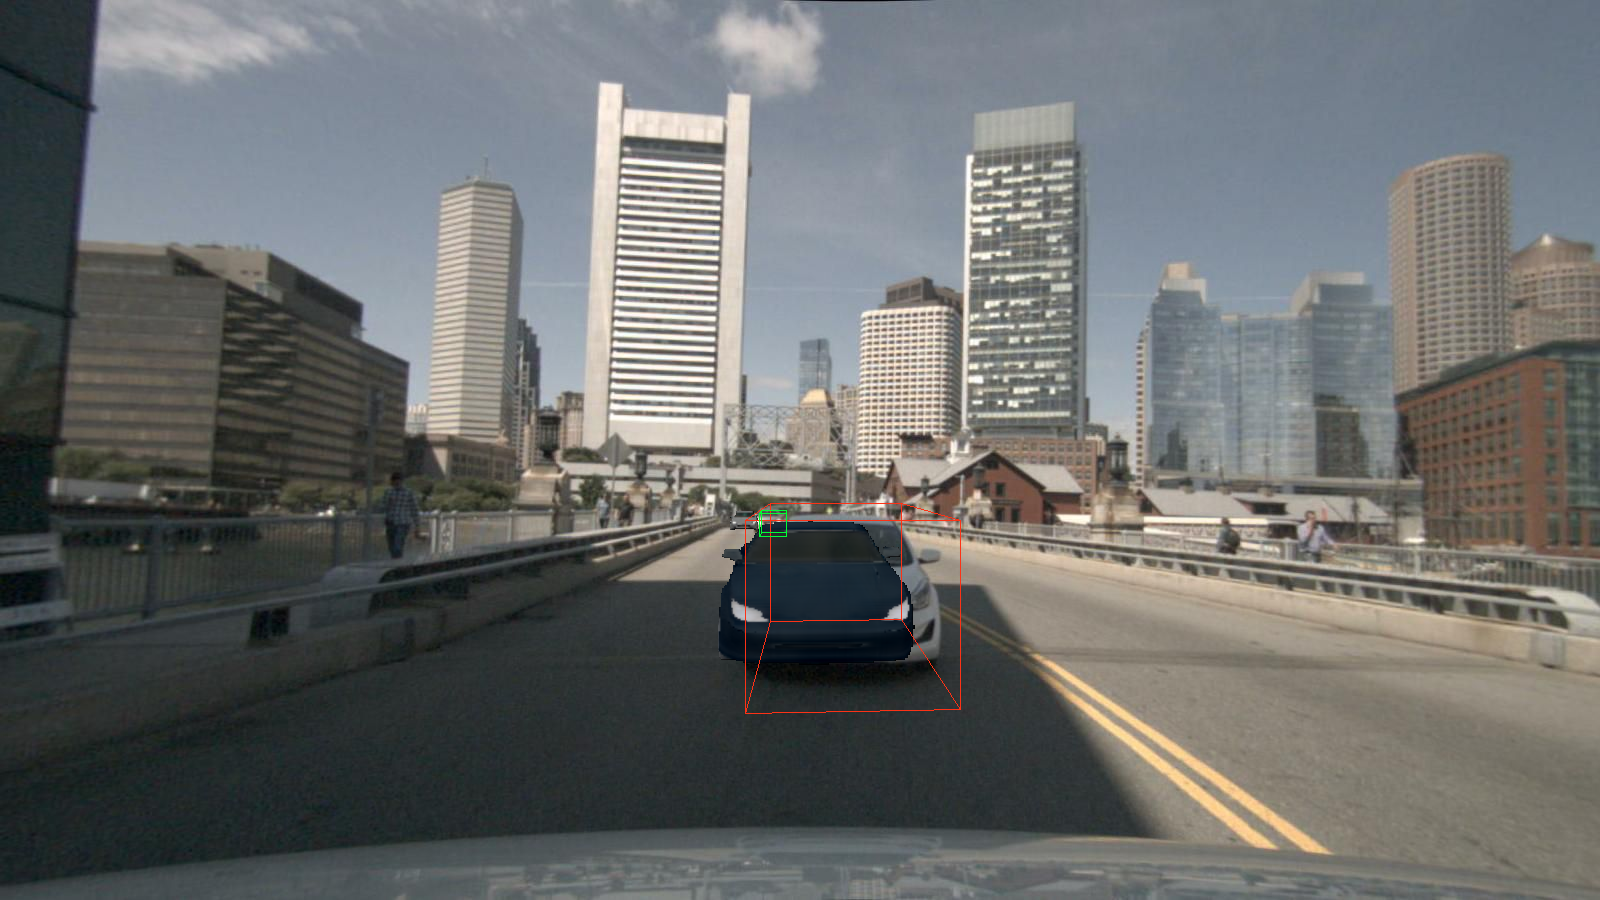
\includegraphics[width=.38\columnwidth, trim={0cm 0cm 0cm 0cm},clip]{fig/additional_nuscenes_results/scene12/22.png}}&
		\raisebox{-0.5\height}{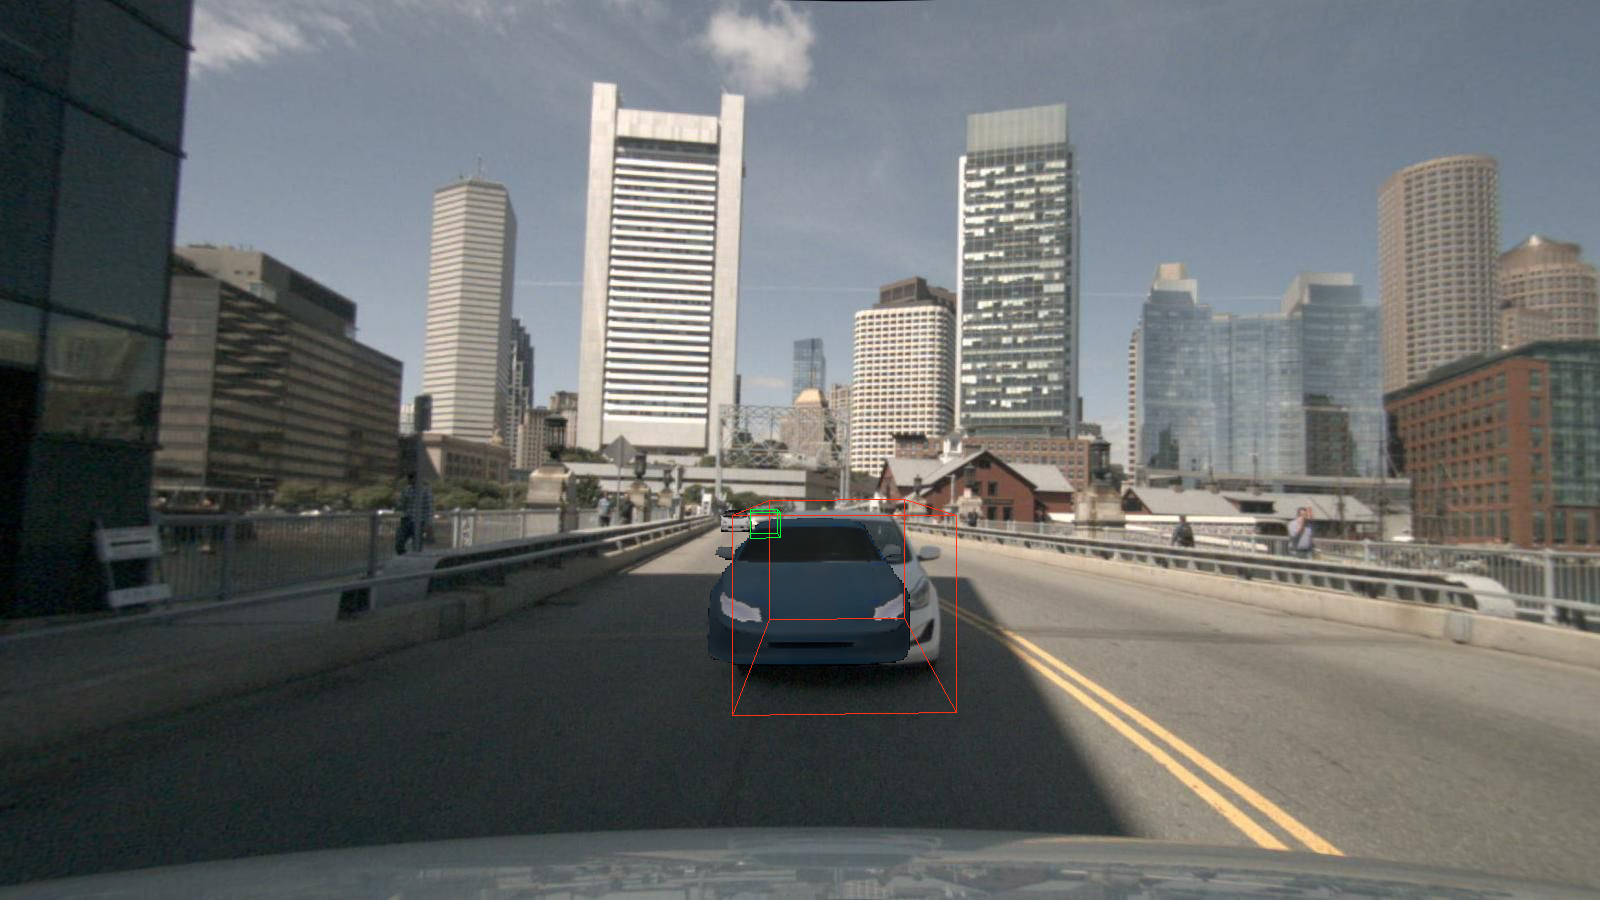
\includegraphics[width=.38\columnwidth, trim={0cm 0cm 0cm 0cm},clip]{fig/additional_nuscenes_results/scene12/23.png}}&
		\raisebox{-0.5\height}{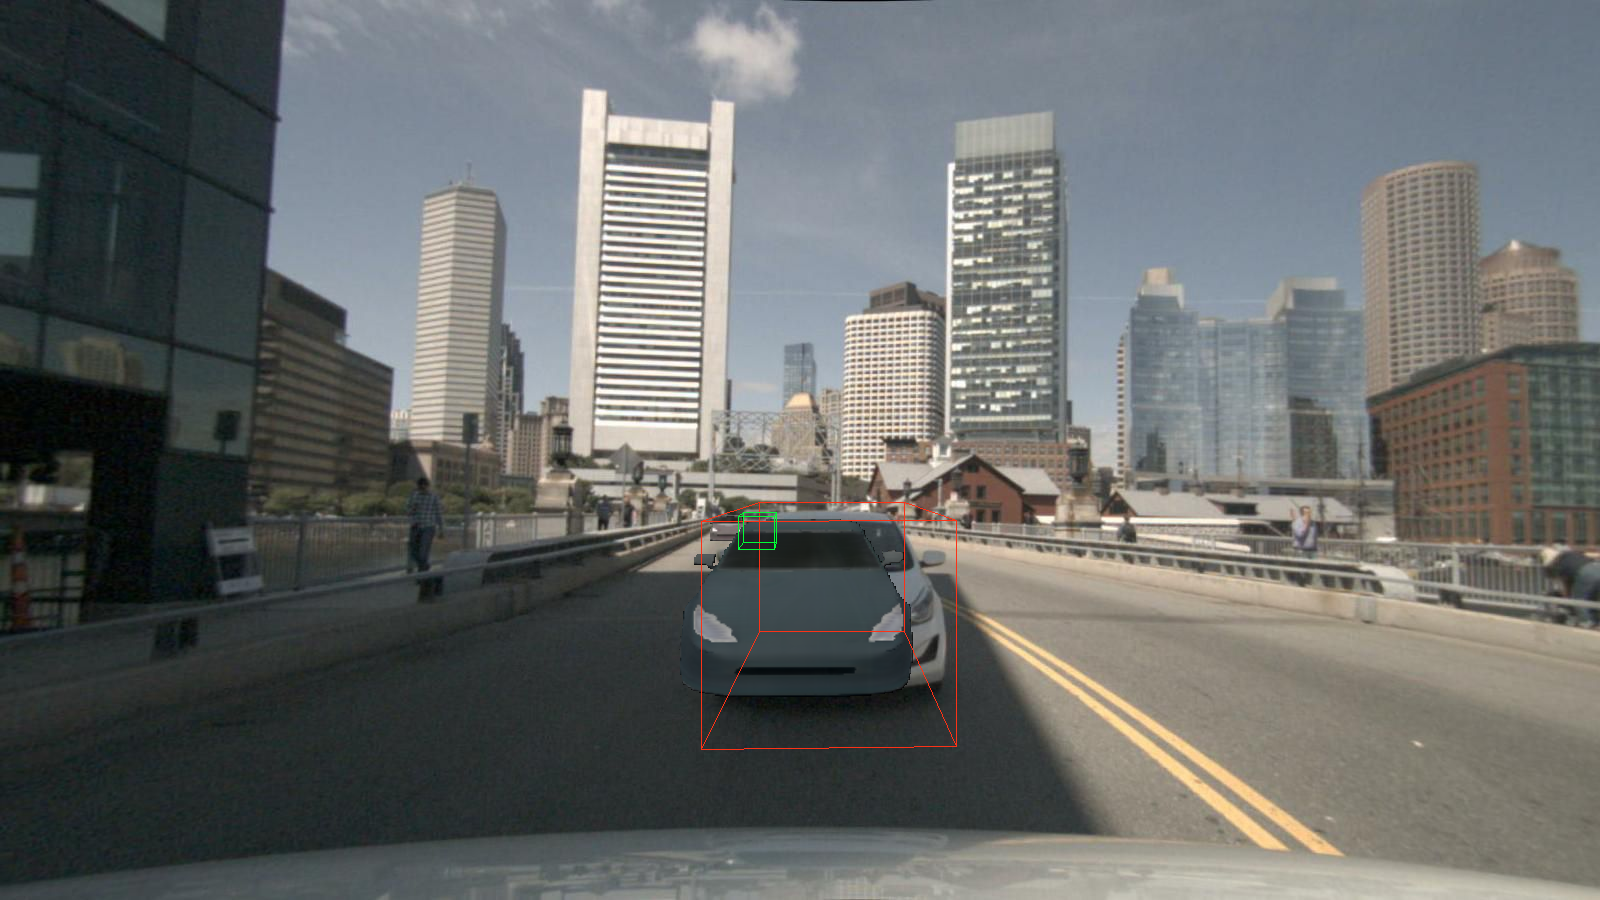
\includegraphics[width=.38\columnwidth, trim={0cm 0cm 0cm 0cm},clip]{fig/additional_nuscenes_results/scene12/4.png}}\\[1.5cm]
  
            \rotatebox[origin=c]{90}{{\Large	Urban 2}}&
  		\raisebox{-0.5\height}{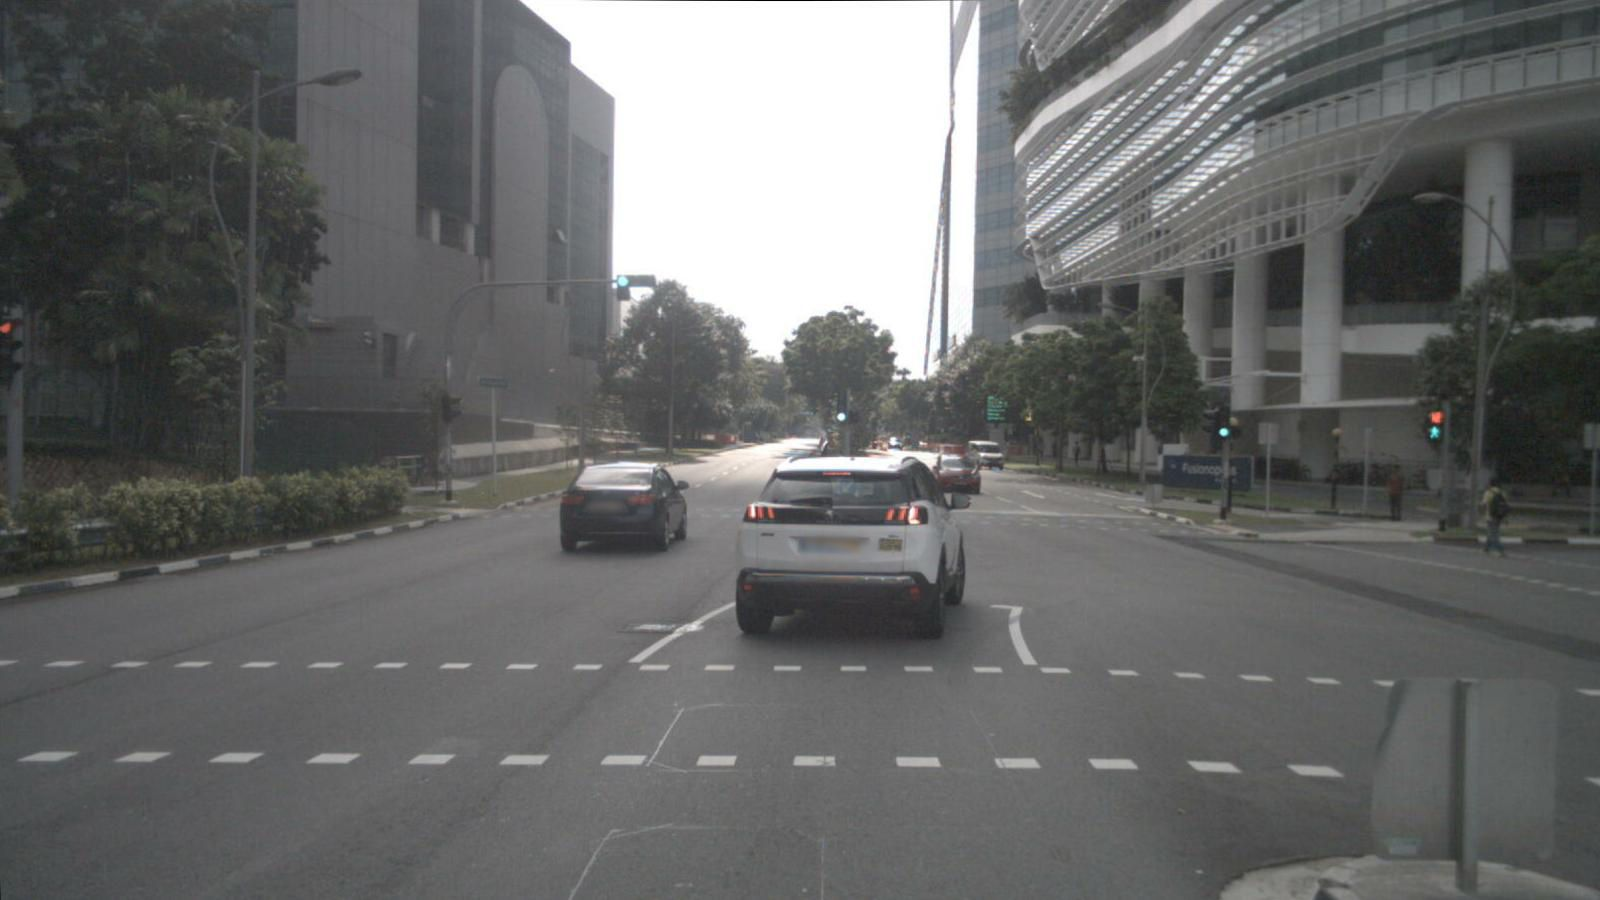
\includegraphics[width=.38\columnwidth, trim={0cm 0cm 0cm 0cm},clip]{fig/additional_nuscenes_results/scene4/2_gt.png}}&
		\raisebox{-0.5\height}{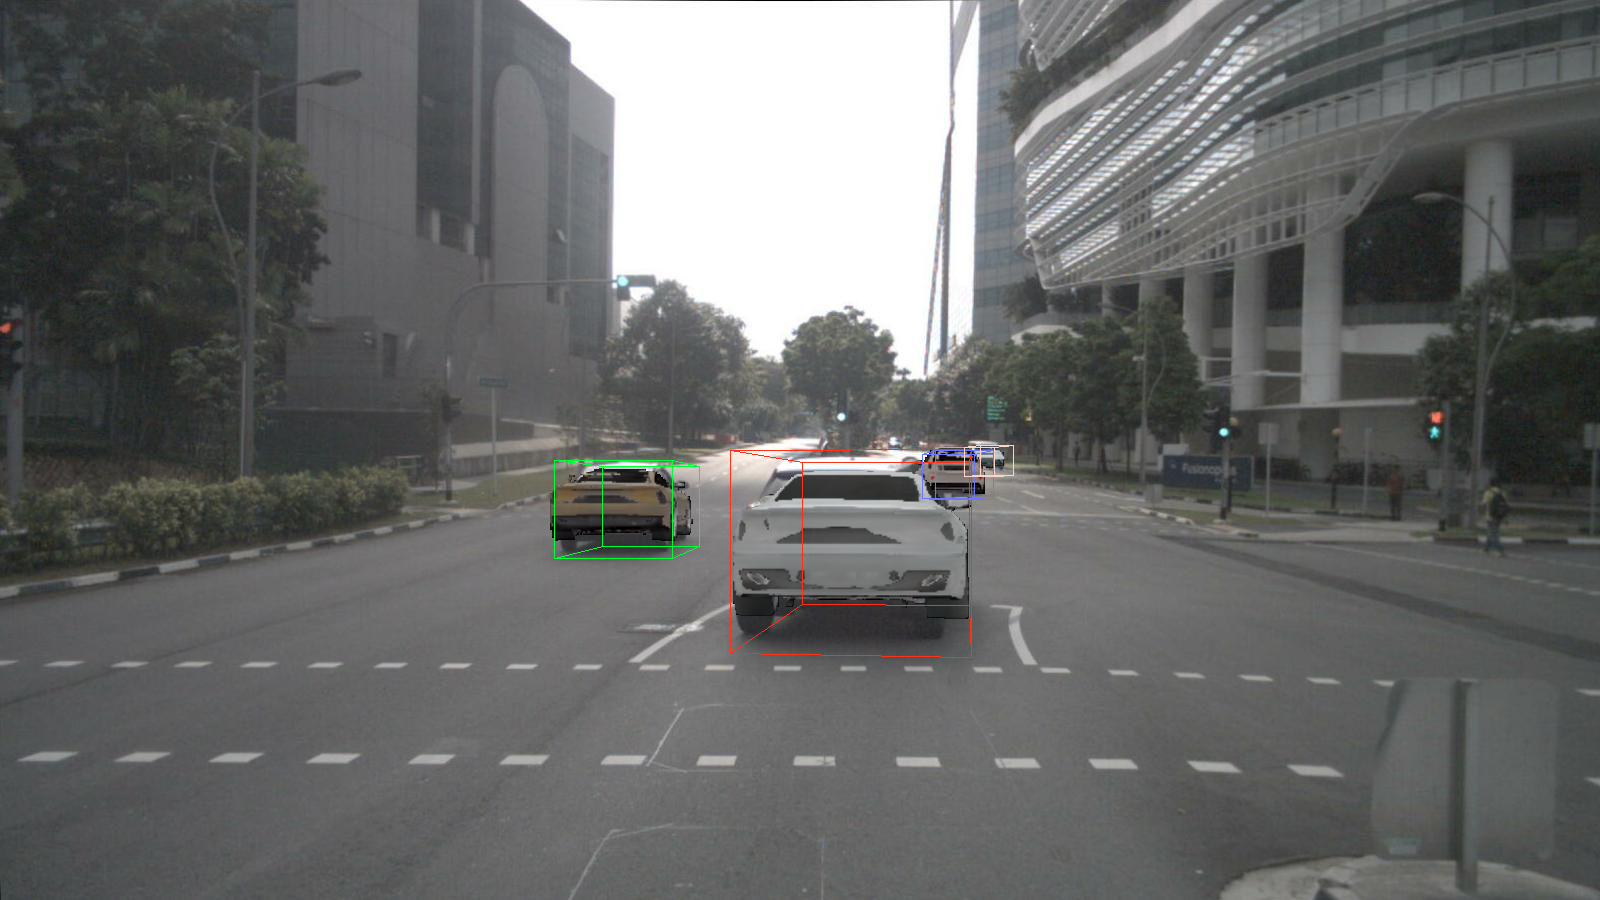
\includegraphics[width=.38\columnwidth, trim={0cm 0cm 0cm 0cm},clip]{fig/additional_nuscenes_results/scene4/2_out.png}}&
		\raisebox{-0.5\height}{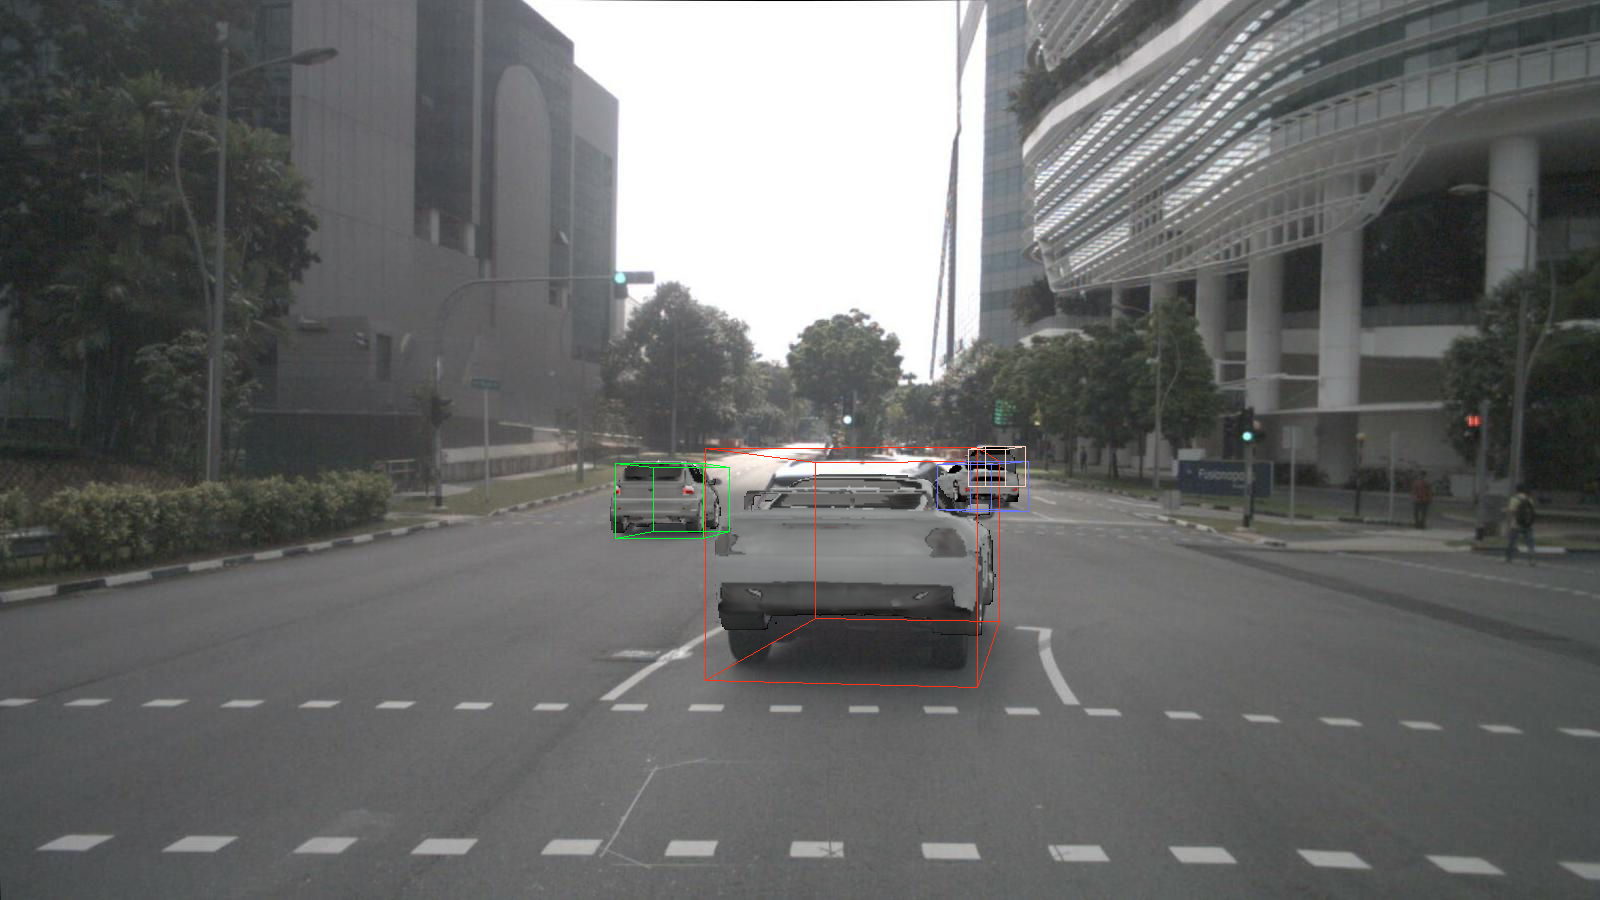
\includegraphics[width=.38\columnwidth, trim={0cm 0cm 0cm 0cm},clip]{fig/additional_nuscenes_results/scene4/3_gt.png}}&
		\raisebox{-0.5\height}{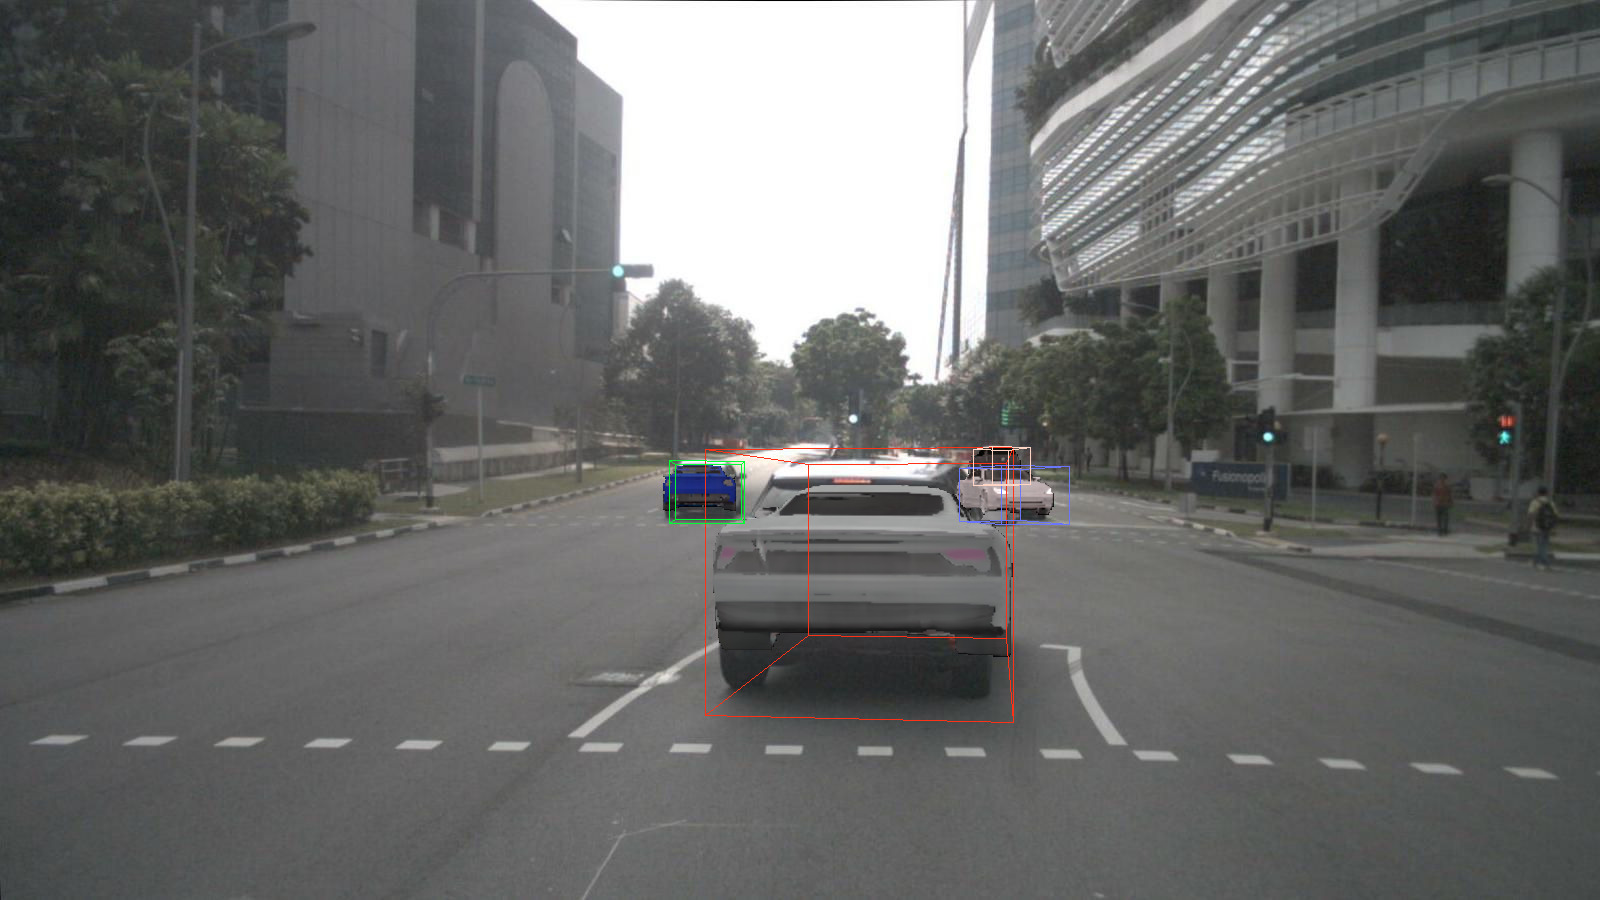
\includegraphics[width=.38\columnwidth, trim={0cm 0cm 0cm 0cm},clip]{fig/additional_nuscenes_results/scene4/4_gt.png}}&
		\raisebox{-0.5\height}{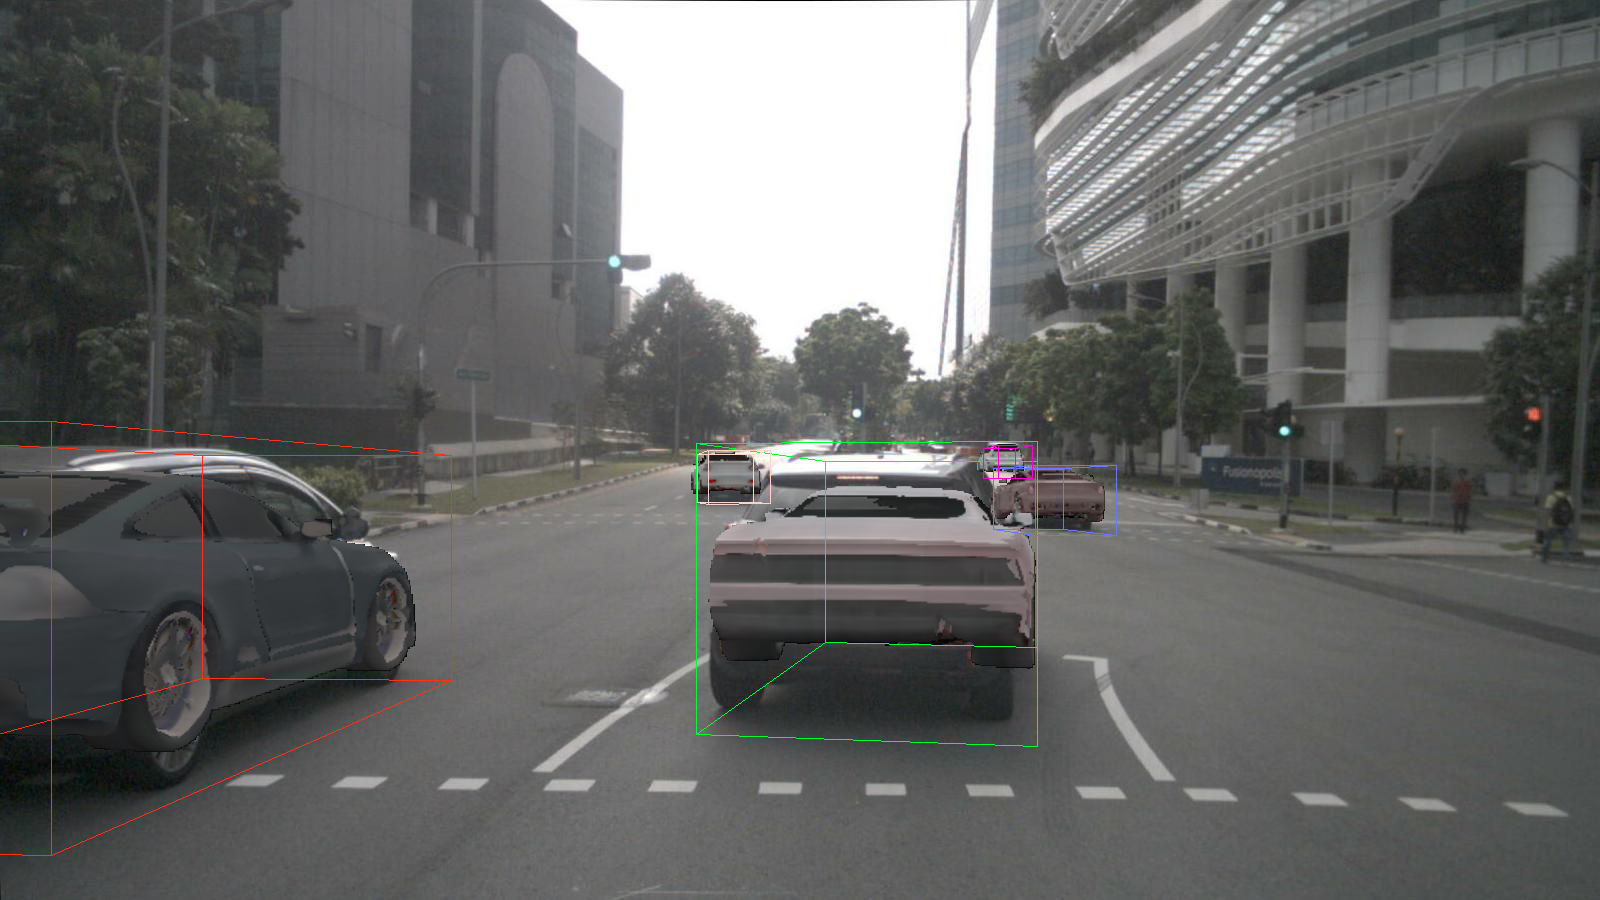
\includegraphics[width=.38\columnwidth, trim={0cm 0cm 0cm 0cm},clip]{fig/additional_nuscenes_results/scene4/5_out.png}}\\[1.5cm]

        \rotatebox[origin=c]{90}{{\Large	 Urban 3}}&
		 \raisebox{-0.5\height}{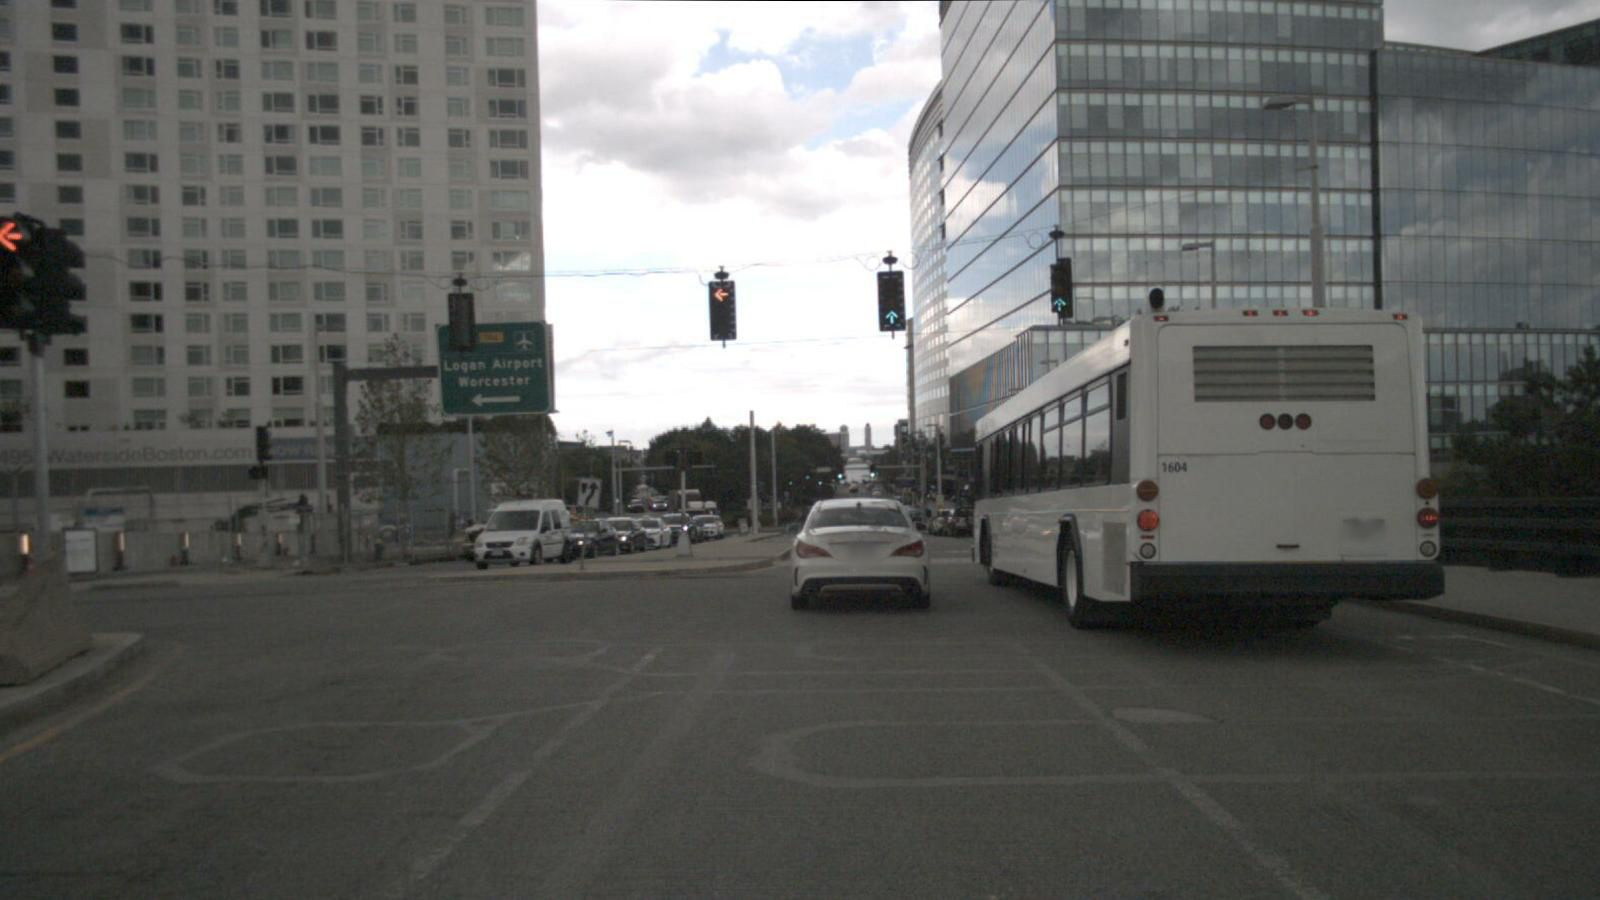
\includegraphics[width=.38\columnwidth, trim={0cm 0cm 0cm 0cm},clip]{fig/additional_nuscenes_results/scene5/0783_0_gt.png}}&
		 \raisebox{-0.5\height}{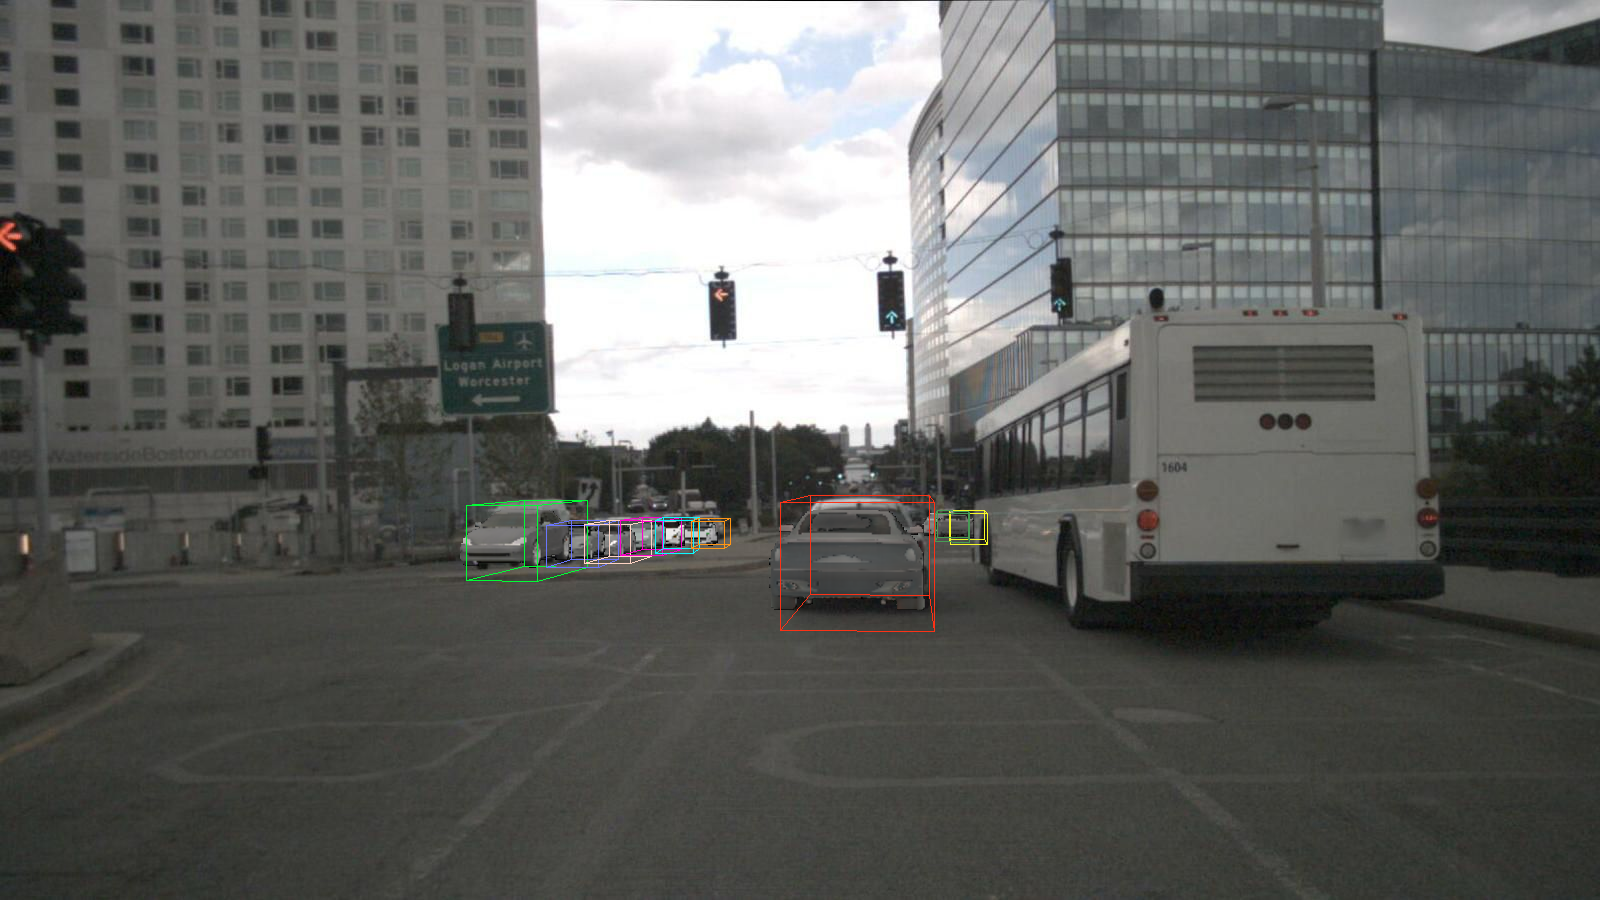
\includegraphics[width=.38\columnwidth, trim={0cm 0cm 0cm 0cm},clip]{fig/additional_nuscenes_results/scene5/0783_0_bbox.png}}&
		 \raisebox{-0.5\height}{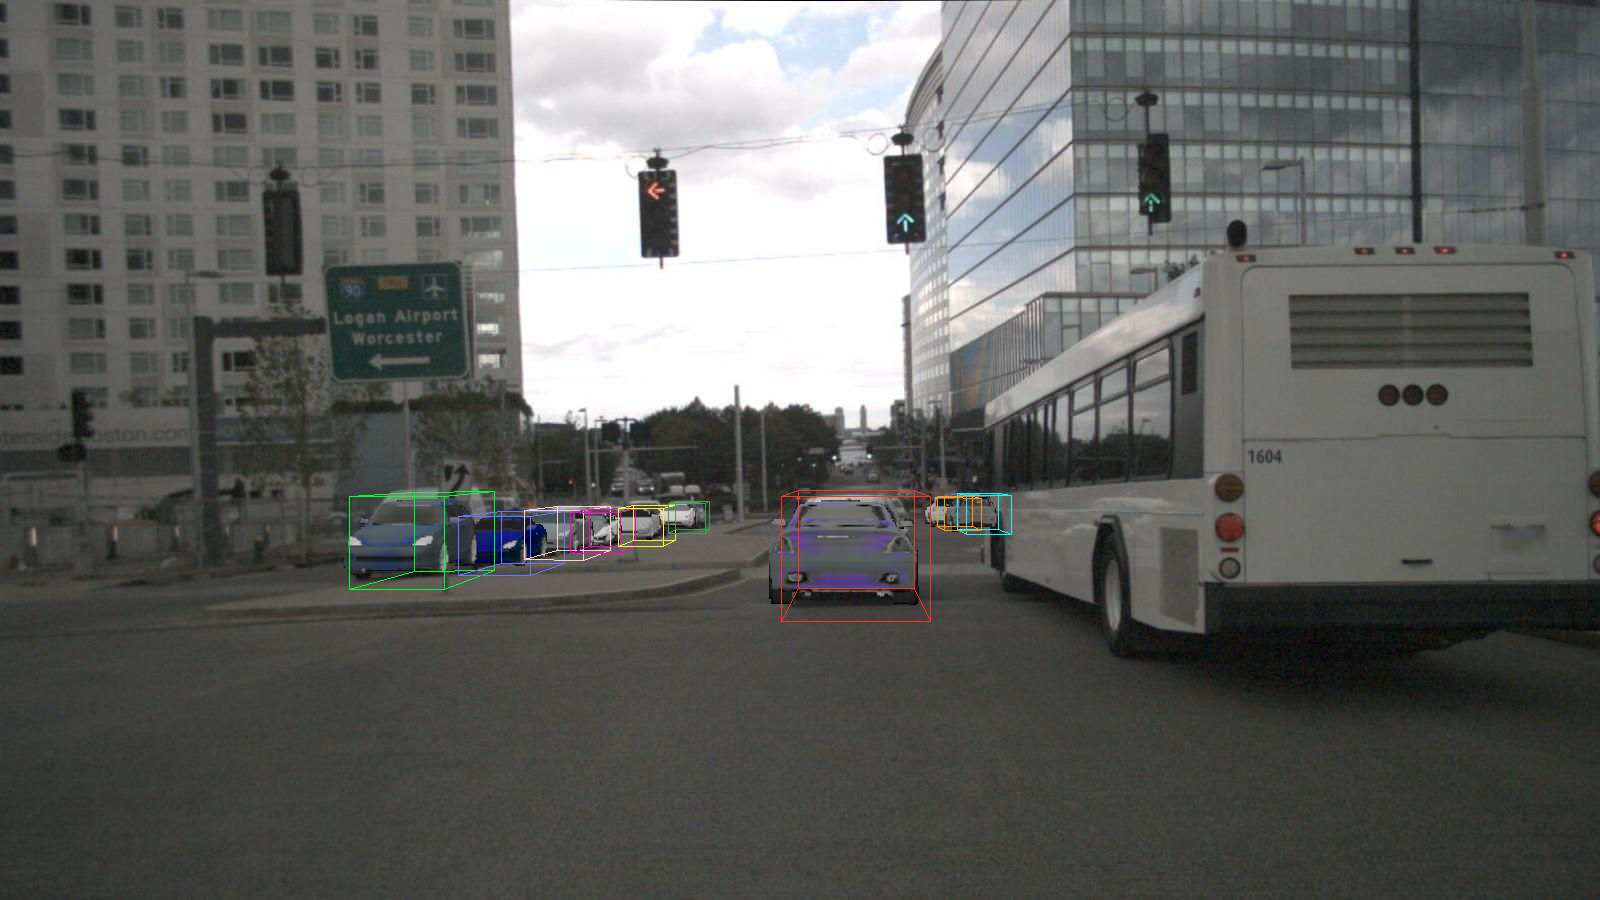
\includegraphics[width=.38\columnwidth, trim={0cm 0cm 0cm 0cm},clip]{fig/additional_nuscenes_results/scene5/0783_1_bbox.png}}&
		 \raisebox{-0.5\height}{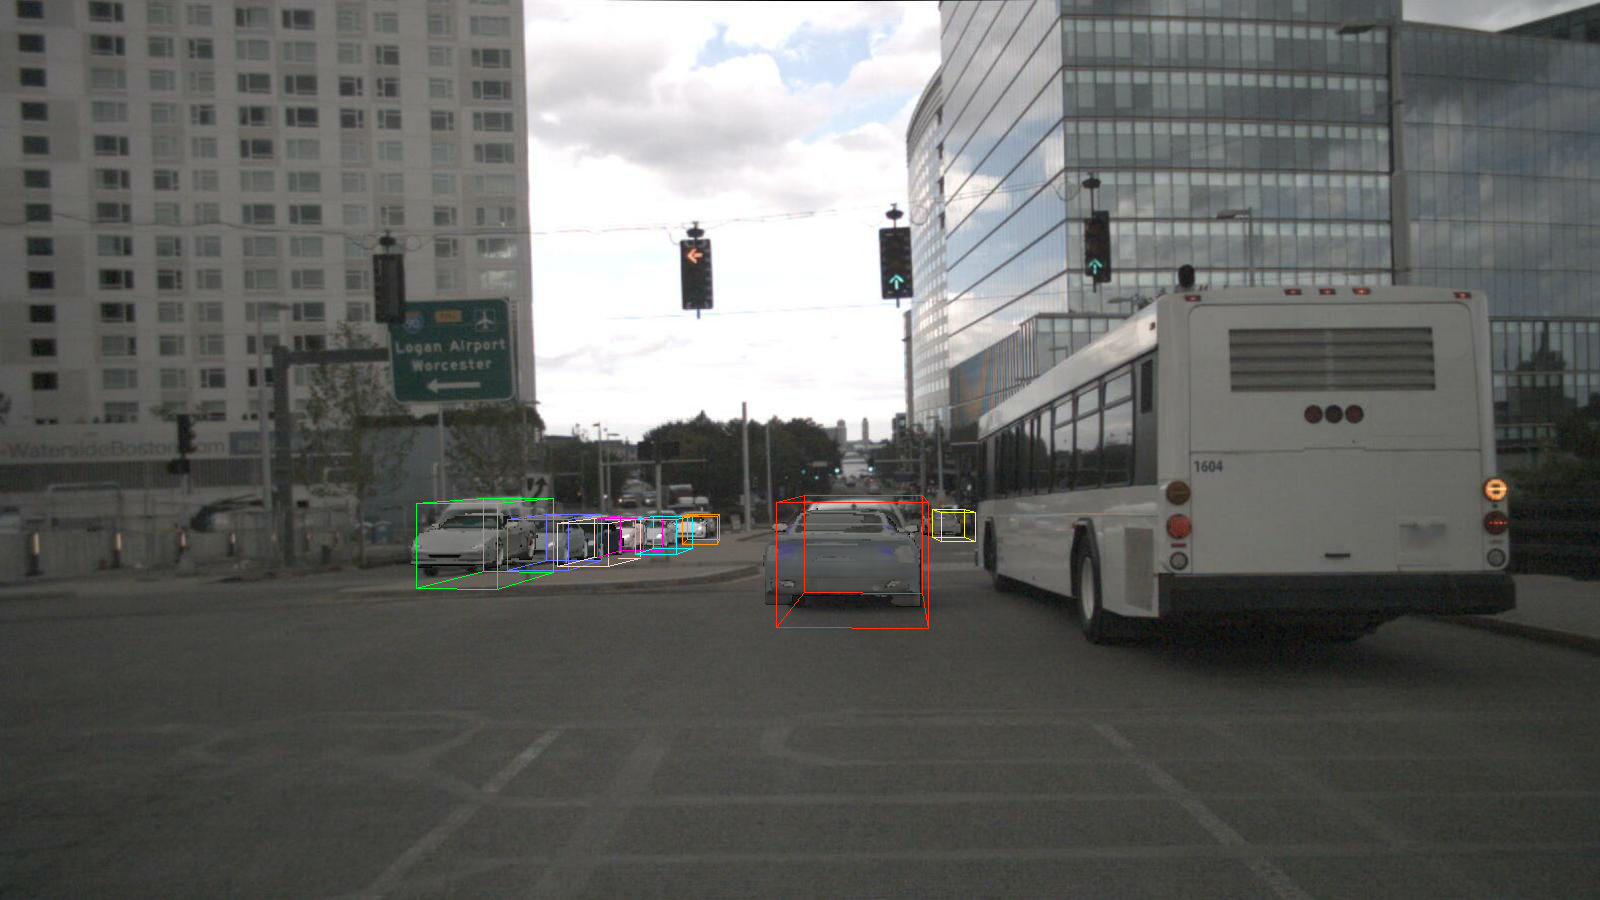
\includegraphics[width=.38\columnwidth, trim={0cm 0cm 0cm 0cm},clip]{fig/additional_nuscenes_results/scene5/0783_2_bbox.png}}&
		 \raisebox{-0.5\height}{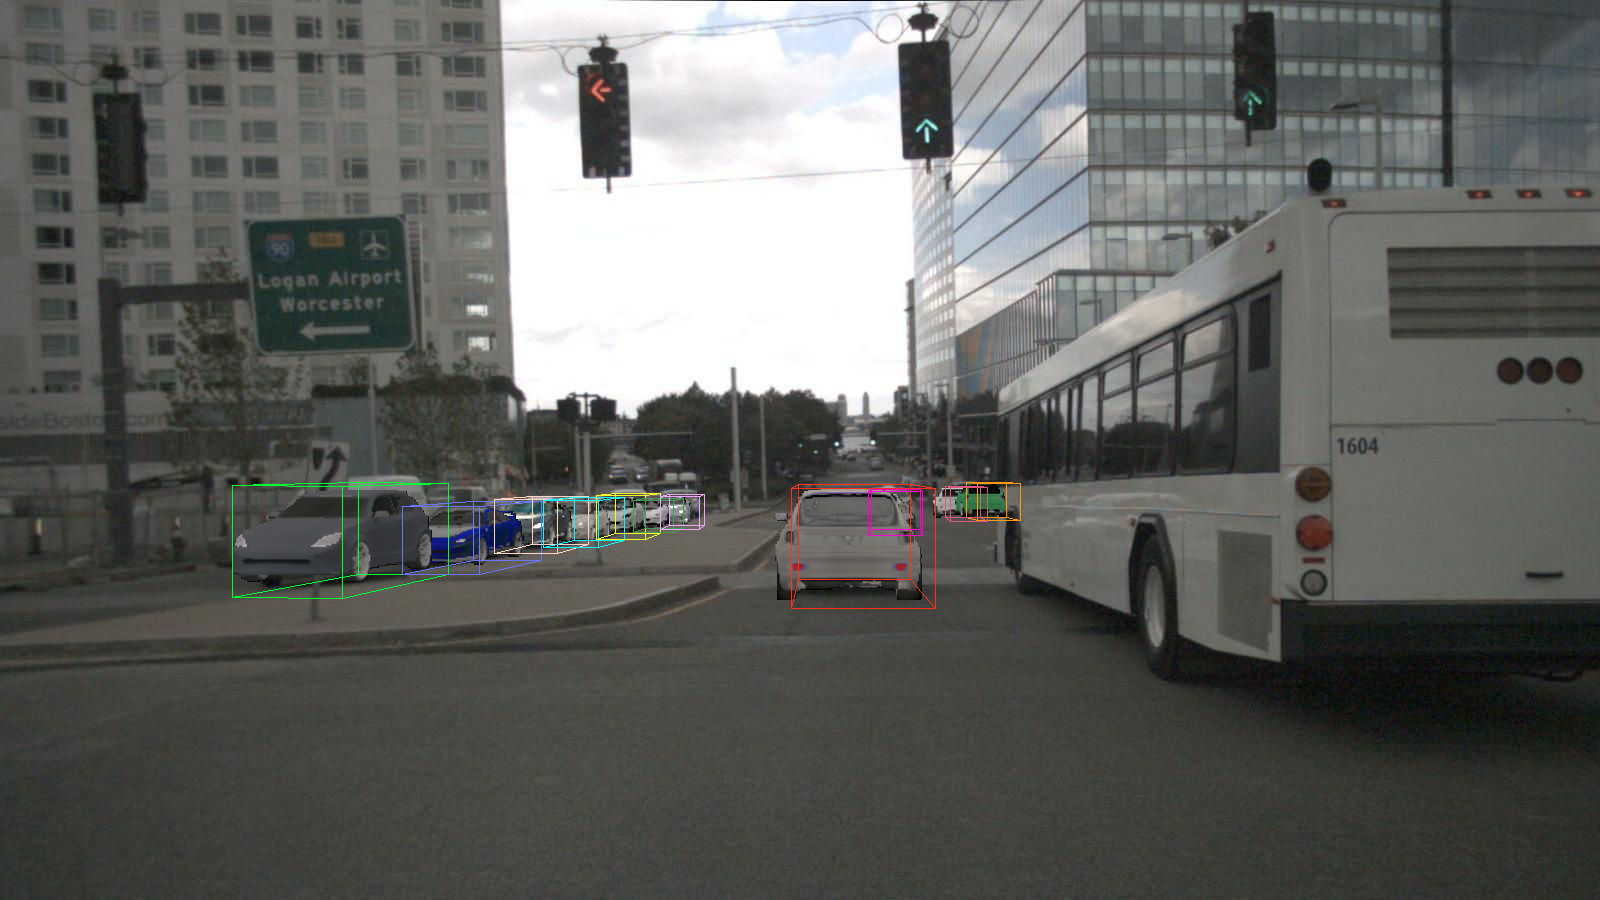
\includegraphics[width=.38\columnwidth, trim={0cm 0cm 0cm 0cm},clip]{fig/additional_nuscenes_results/scene5/0783_3_bbox.png}}\\[1.5cm]
        
    \rotatebox[origin=c]{90}{{\Large	  Crossing}}&
		 \raisebox{-0.5\height}{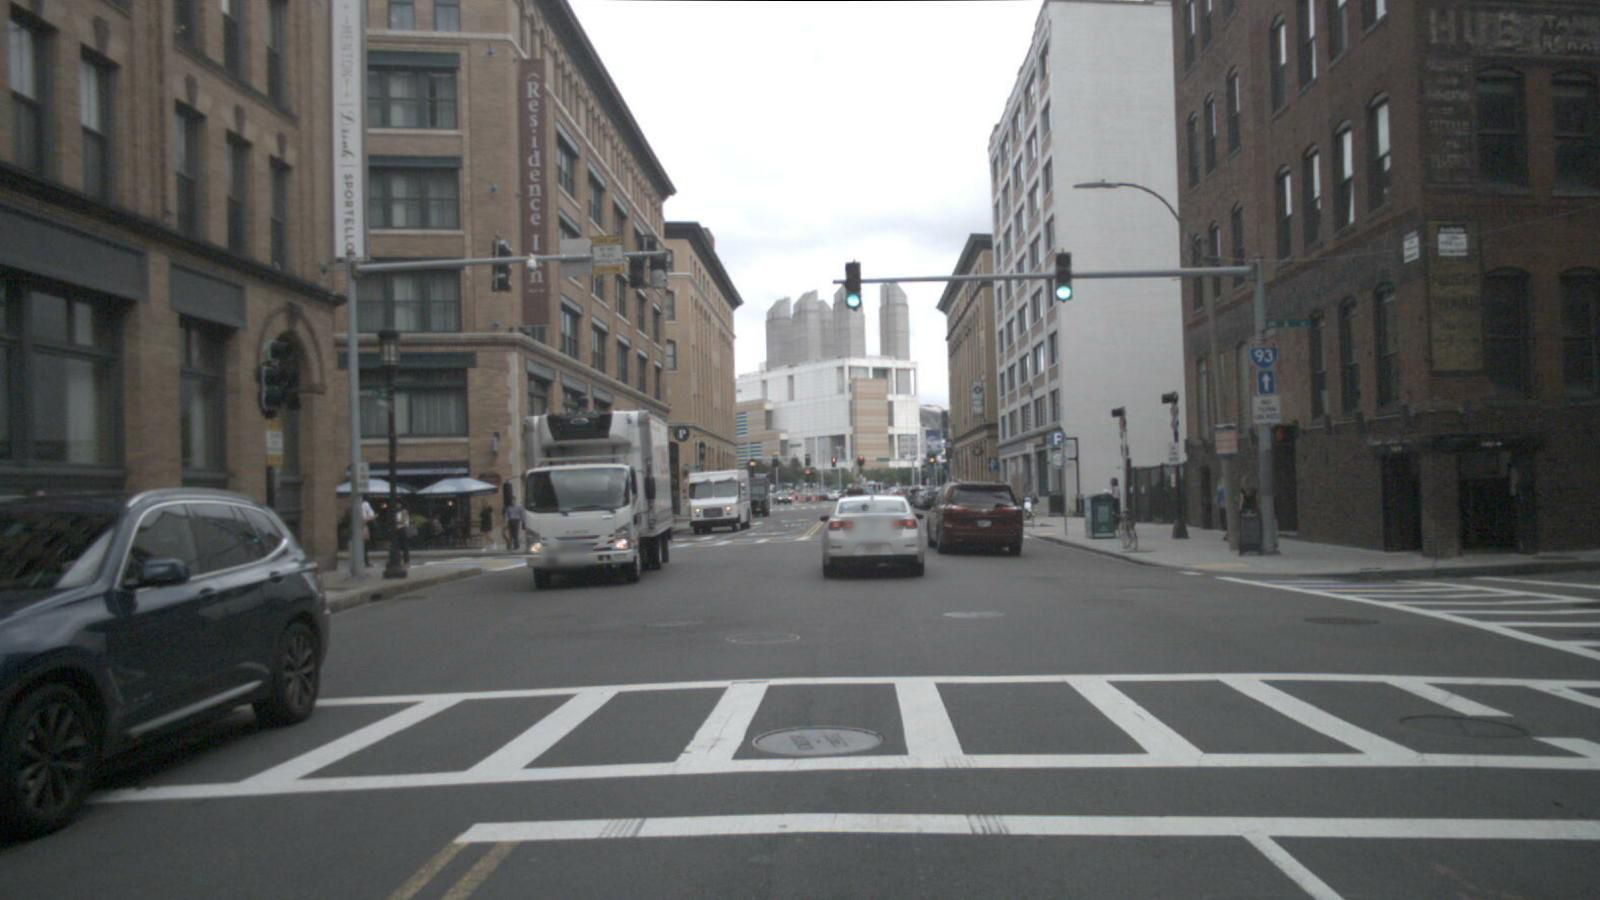
\includegraphics[width=.38\columnwidth, trim={0cm 0cm 0cm 0cm},clip]{fig/additional_nuscenes_results/scene6/0104_8_gt.png}}&
		 \raisebox{-0.5\height}{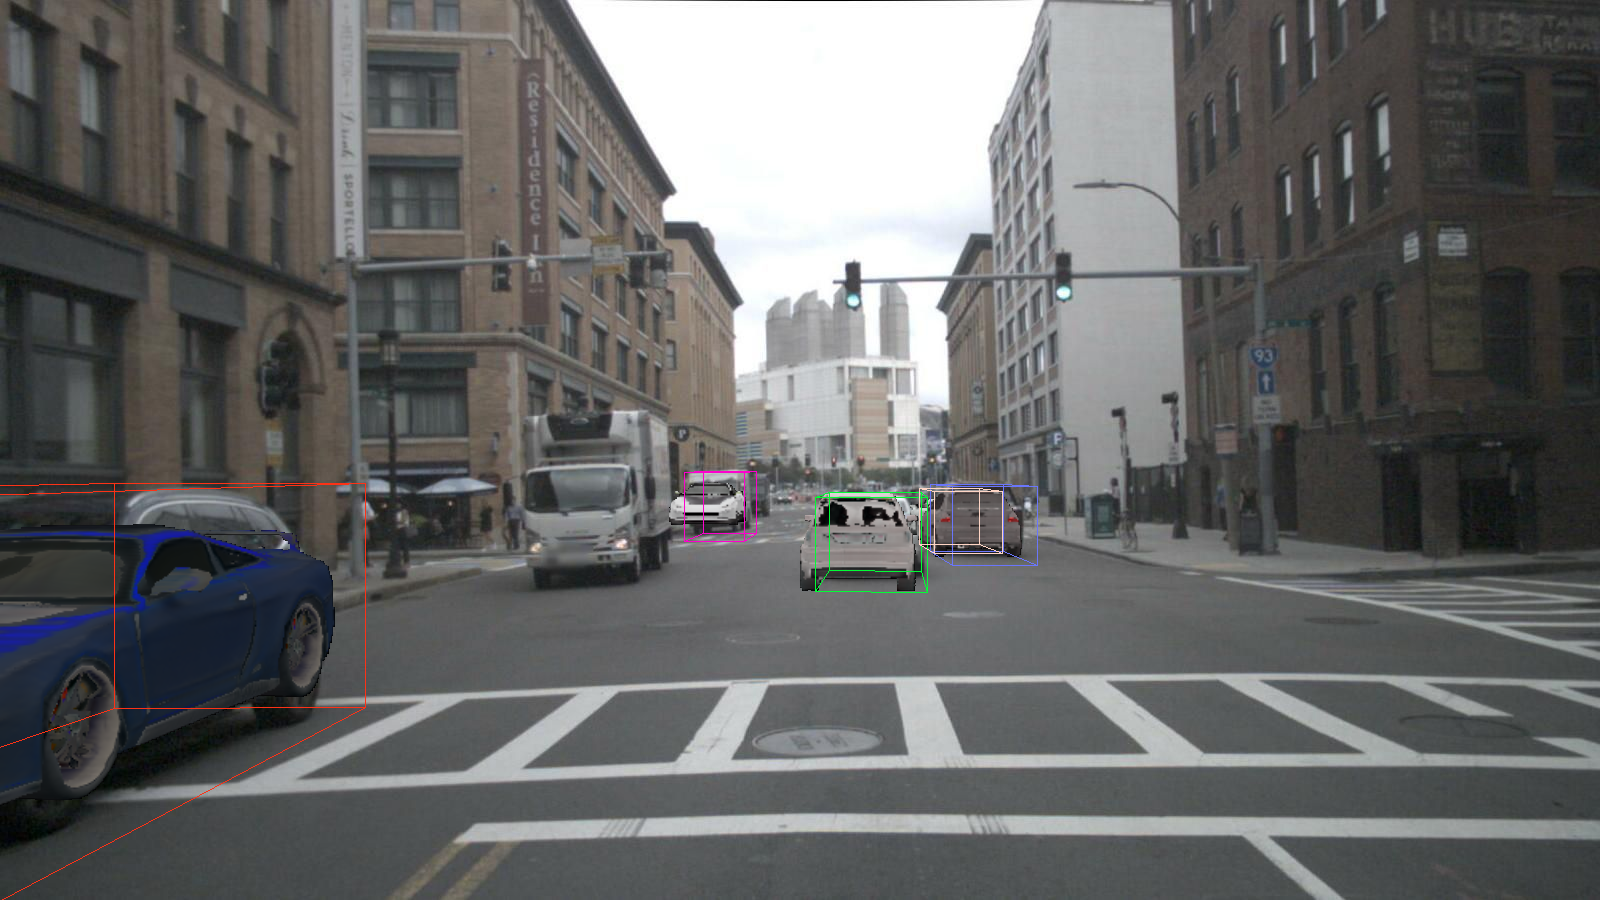
\includegraphics[width=.38\columnwidth, trim={0cm 0cm 0cm 0cm},clip]{fig/additional_nuscenes_results/scene6/0104_8_bbox.png}}&
		 \raisebox{-0.5\height}{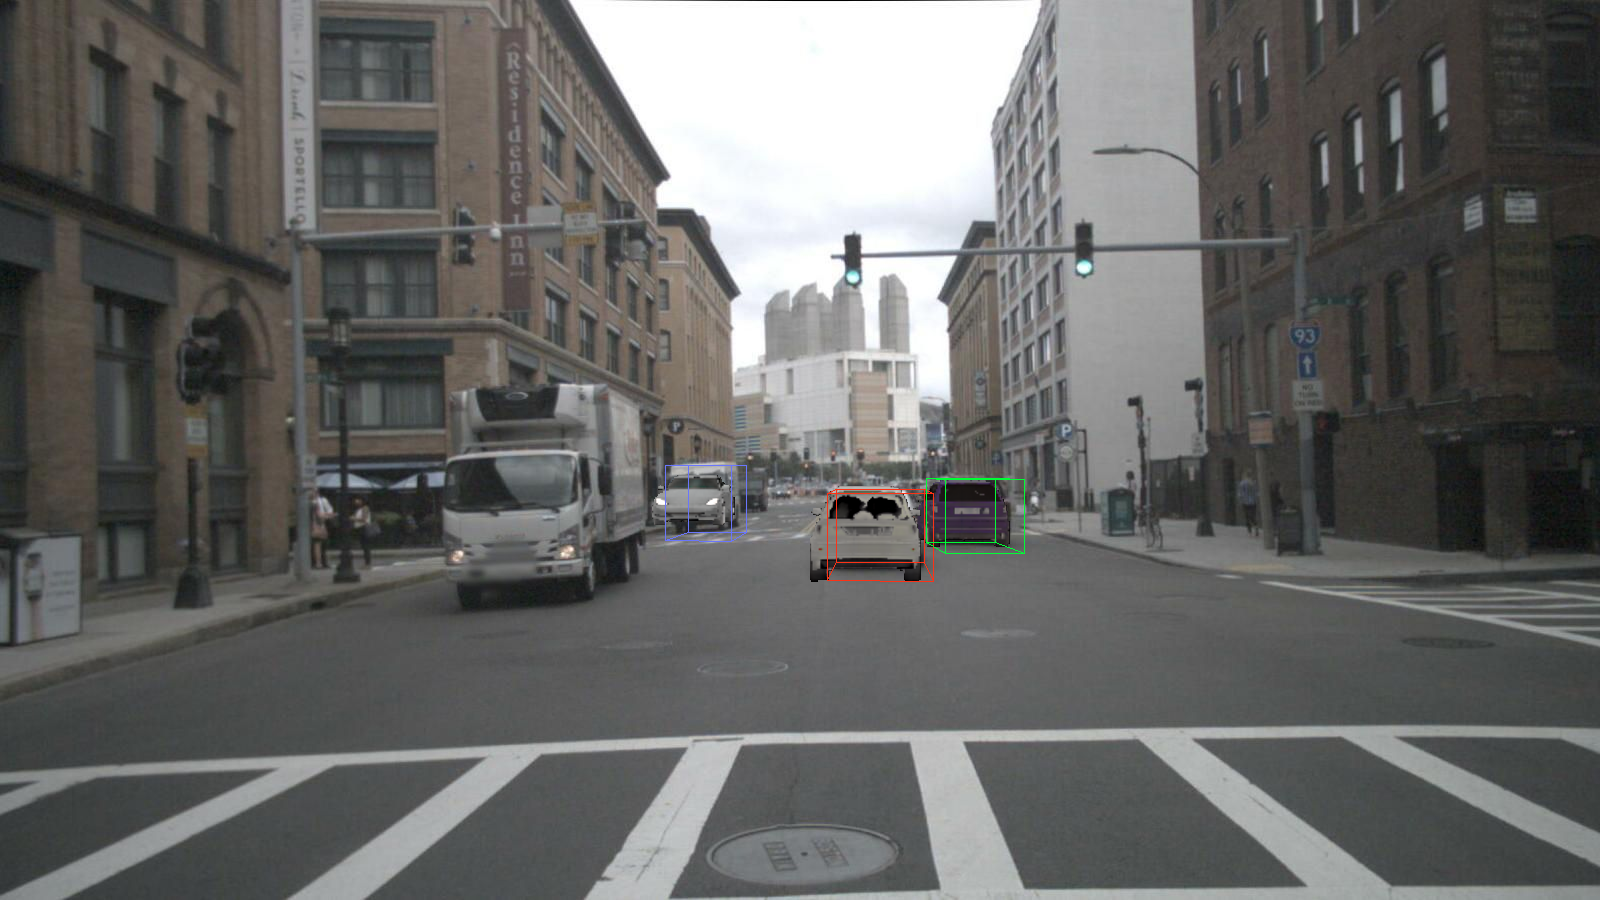
\includegraphics[width=.38\columnwidth, trim={0cm 0cm 0cm 0cm},clip]{fig/additional_nuscenes_results/scene6/0104_9_bbox.png}}&
		 \raisebox{-0.5\height}{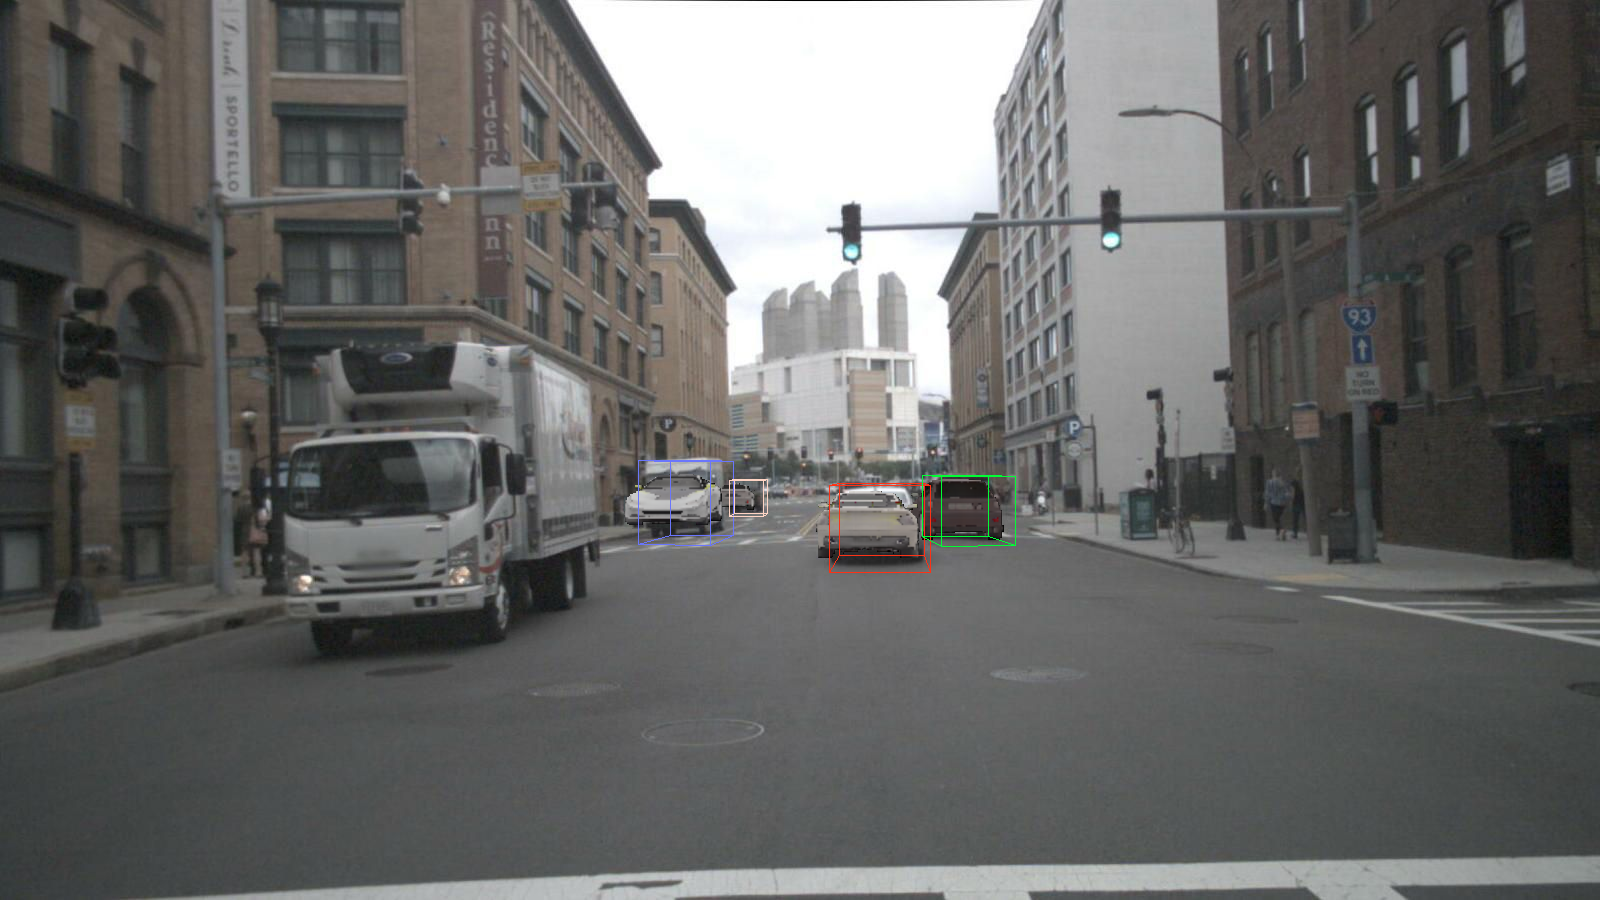
\includegraphics[width=.38\columnwidth, trim={0cm 0cm 0cm 0cm},clip]{fig/additional_nuscenes_results/scene6/0104_10_bbox.png}}&
		 \raisebox{-0.5\height}{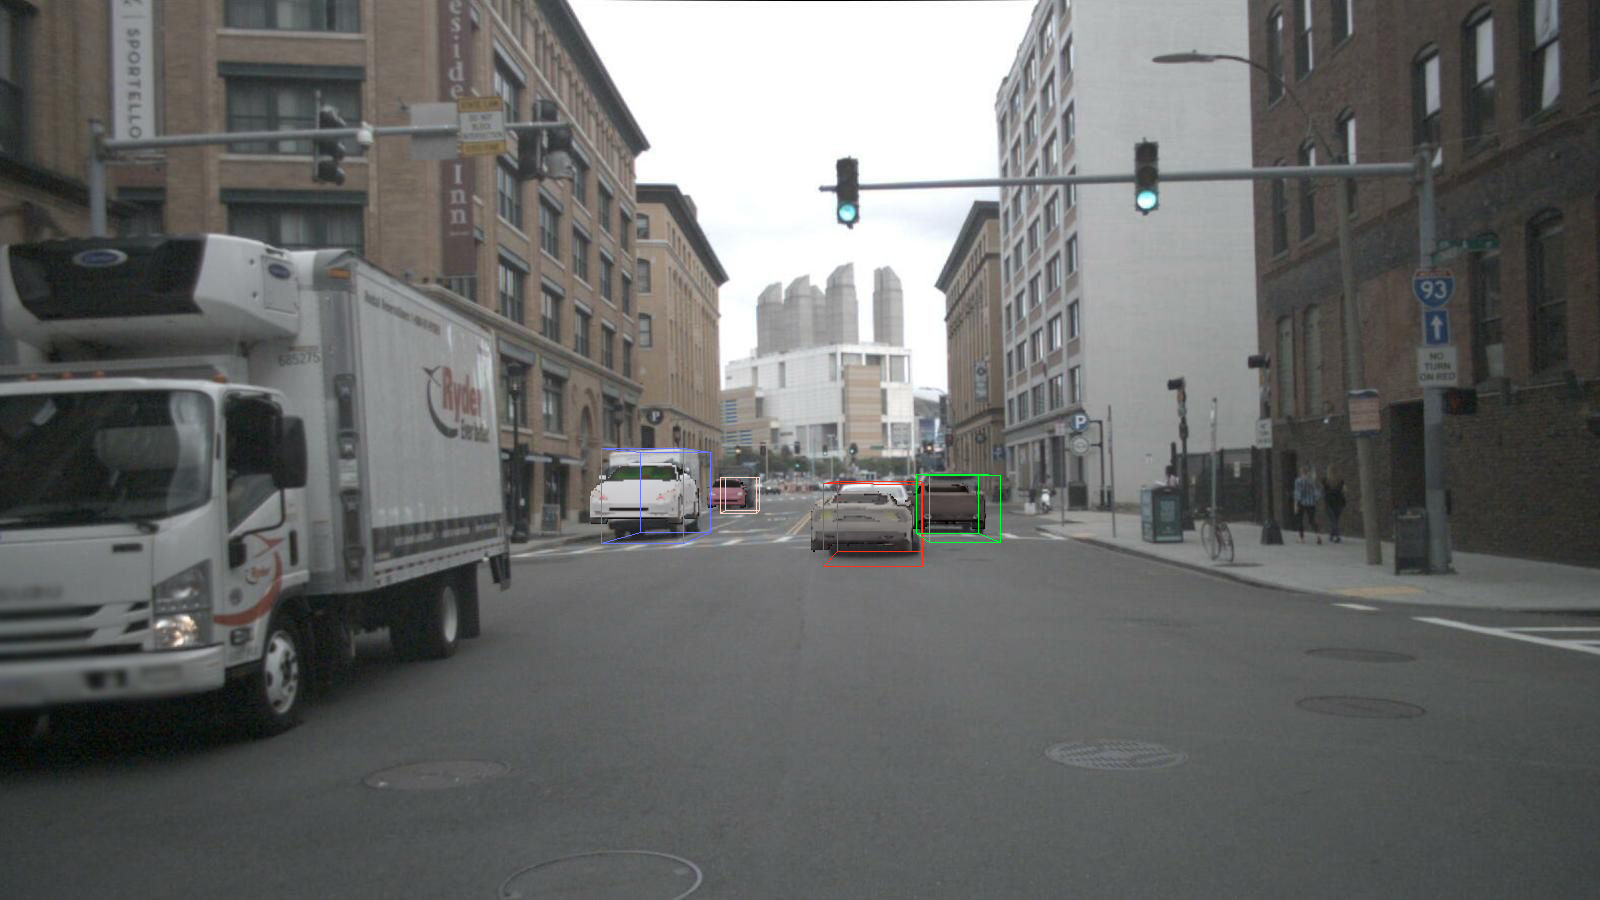
\includegraphics[width=.38\columnwidth, trim={0cm 0cm 0cm 0cm},clip]{fig/additional_nuscenes_results/scene6/0104_11_bbox.png}}\\[1.5cm]

    \rotatebox[origin=c]{90}{{\Large	  Crossing 2}}&
		 \raisebox{-0.5\height}{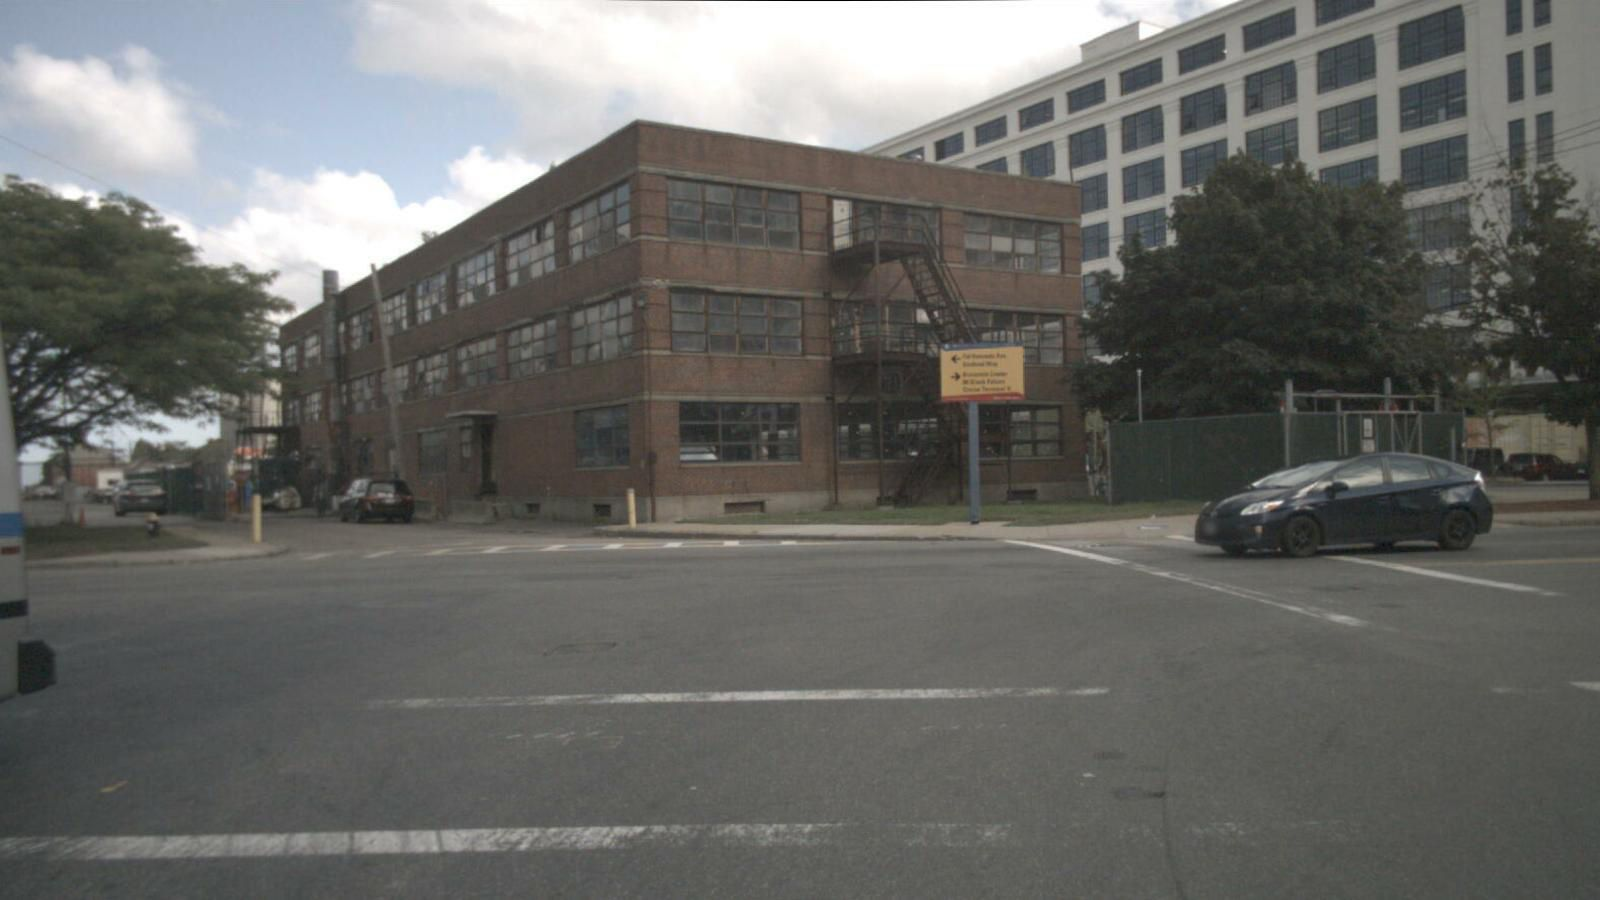
\includegraphics[width=.38\columnwidth, trim={0cm 0cm 0cm 0cm},clip]{fig/additional_nuscenes_results/scene11/gt_img.png}}&
		 \raisebox{-0.5\height}{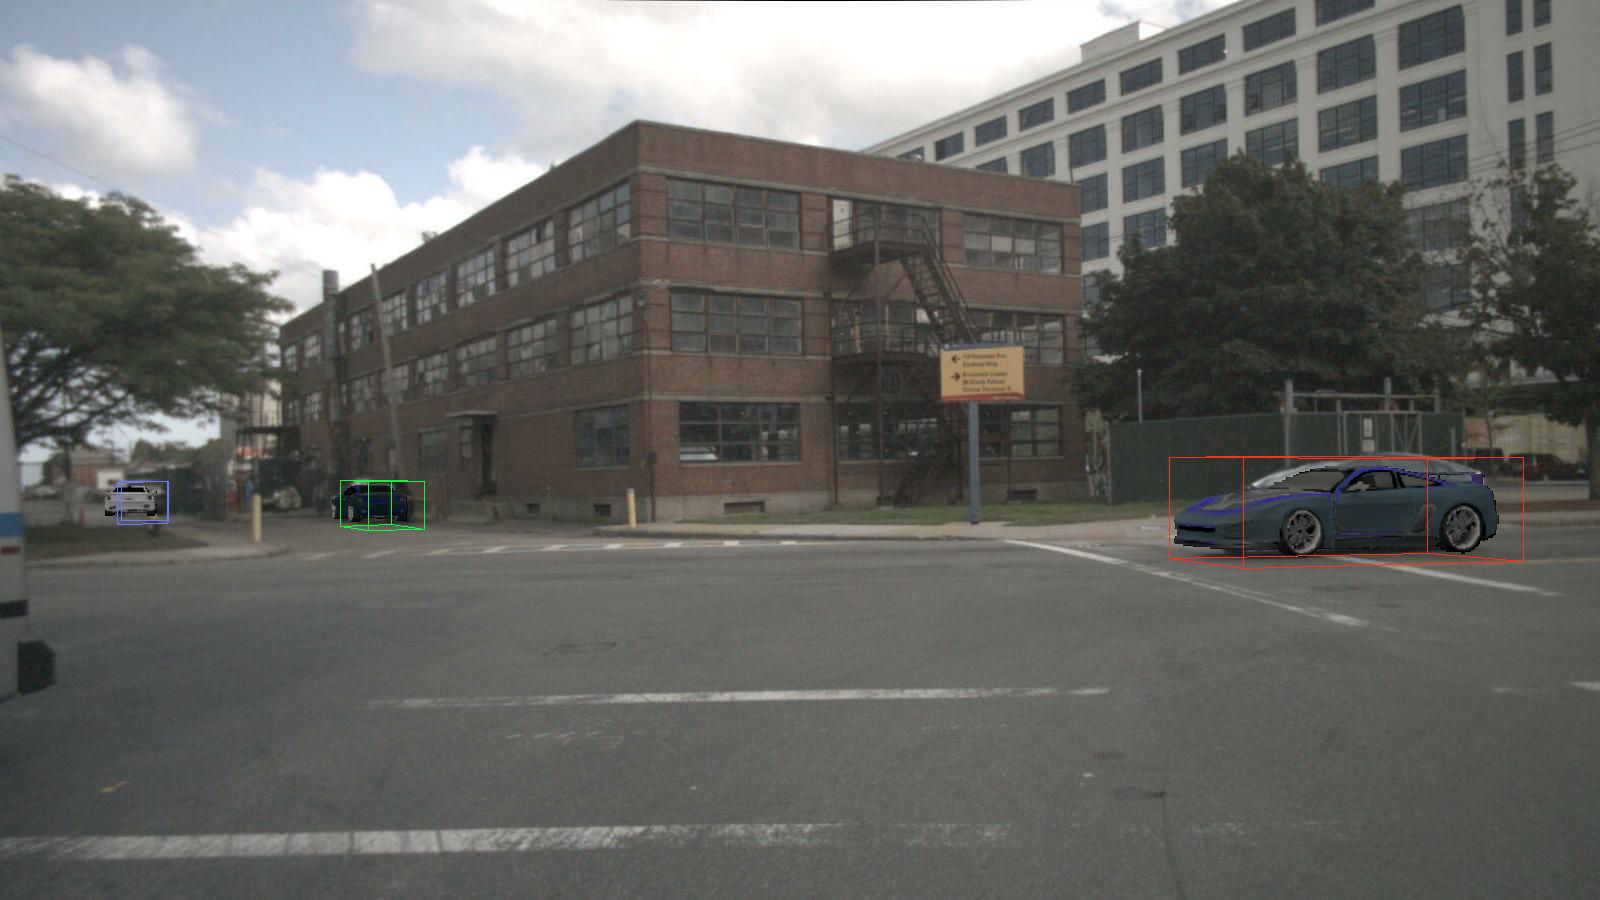
\includegraphics[width=.38\columnwidth, trim={0cm 0cm 0cm 0cm},clip]{fig/additional_nuscenes_results/scene11/27.png}}&
		 \raisebox{-0.5\height}{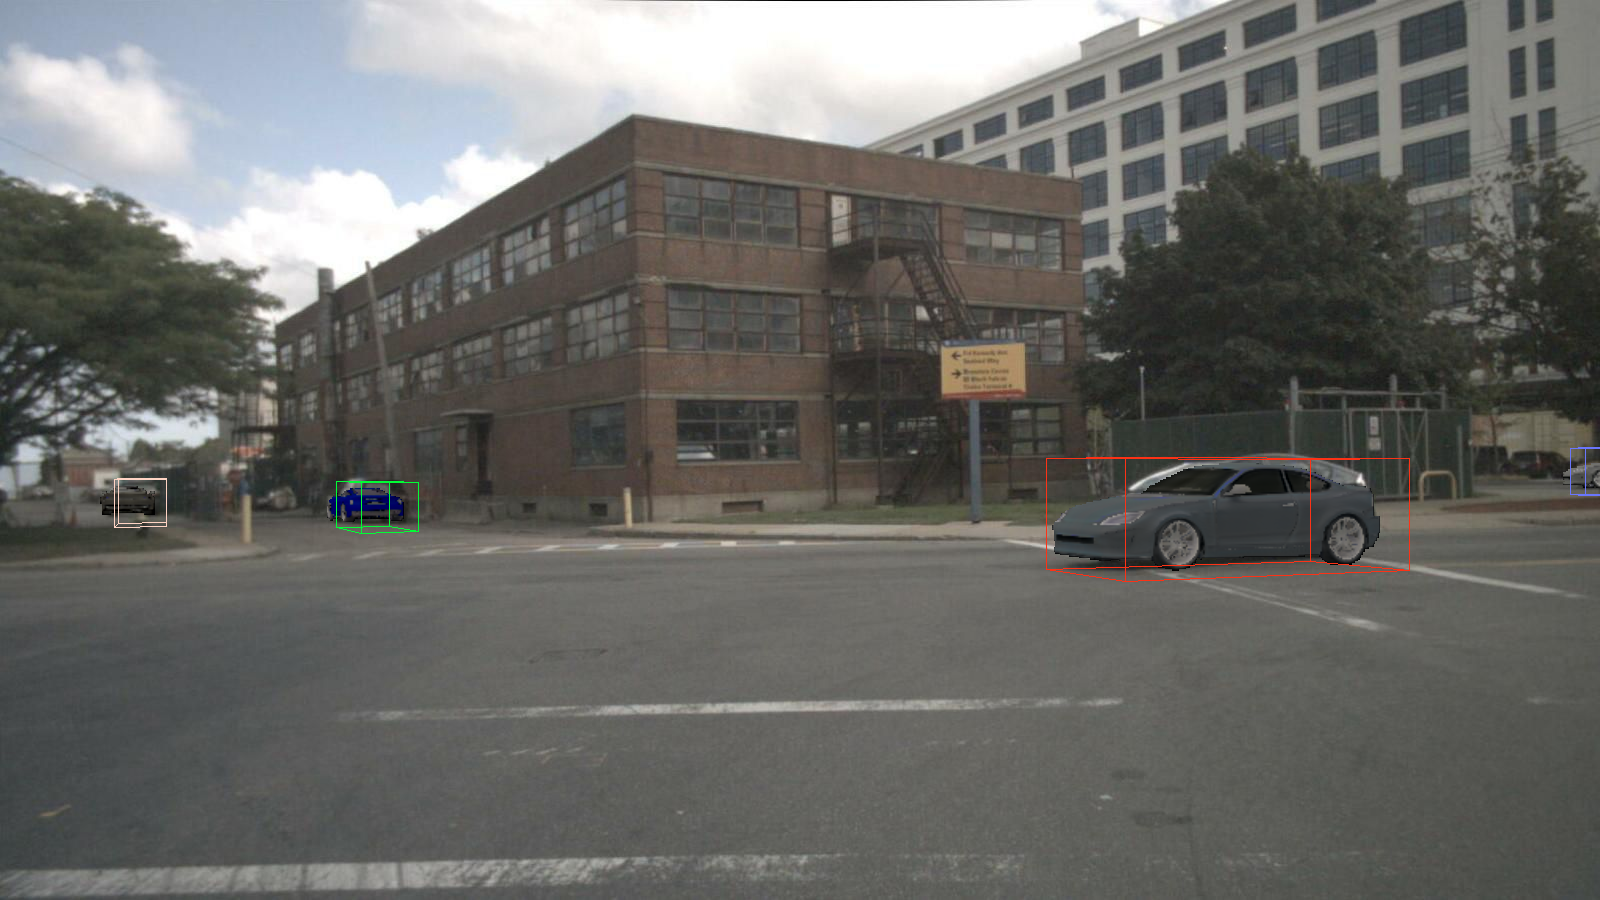
\includegraphics[width=.38\columnwidth, trim={0cm 0cm 0cm 0cm},clip]{fig/additional_nuscenes_results/scene11/28.png}}&
		 \raisebox{-0.5\height}{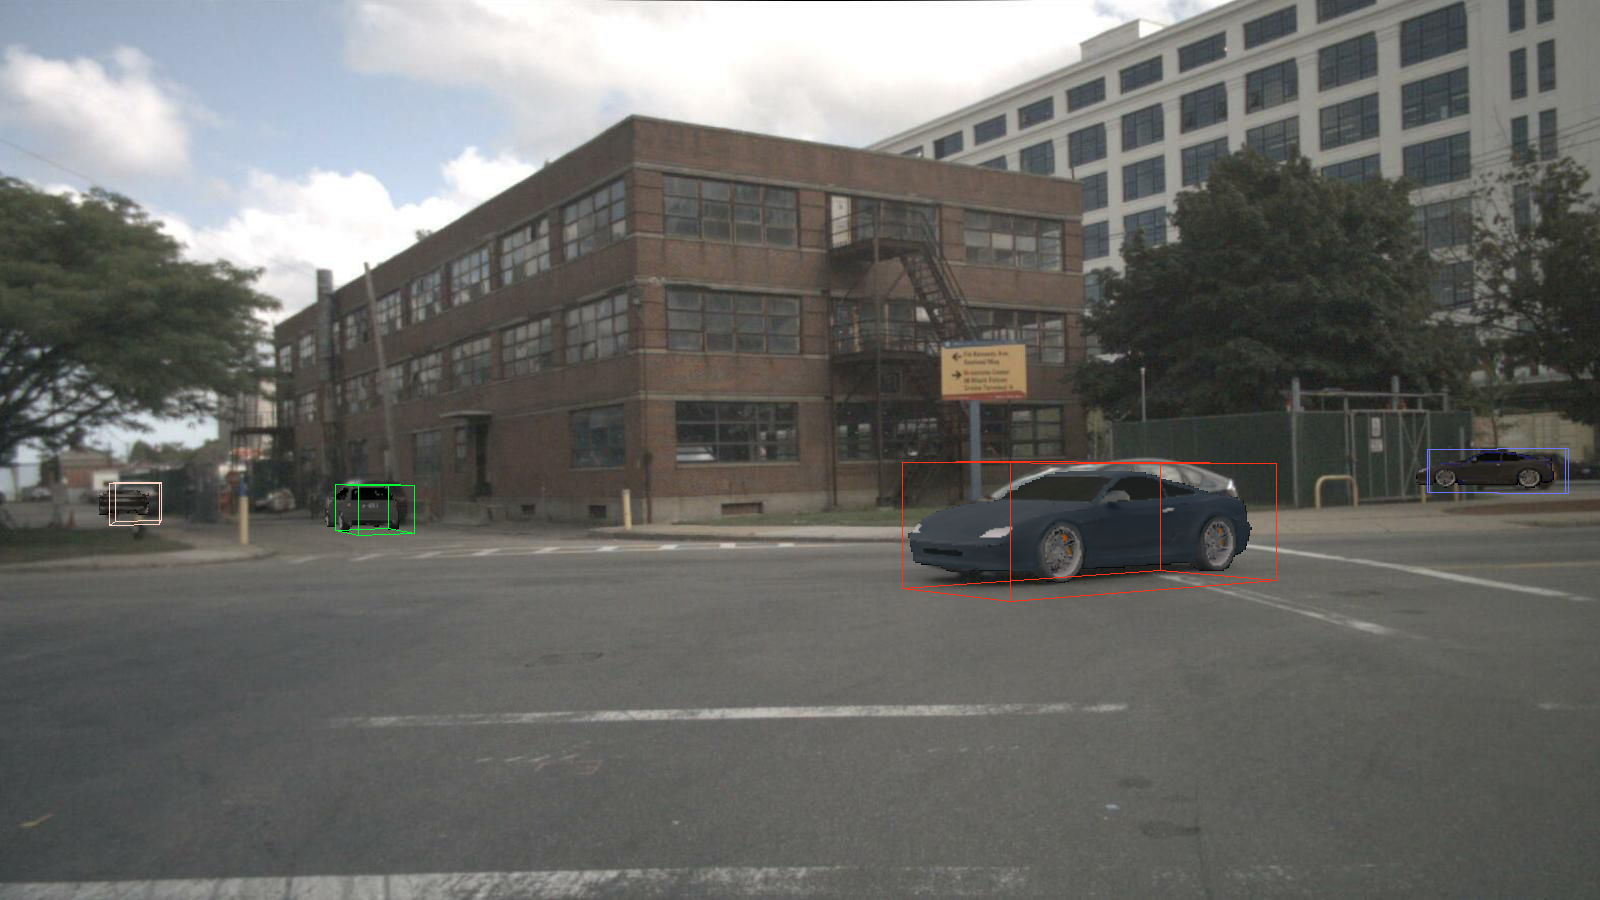
\includegraphics[width=.38\columnwidth, trim={0cm 0cm 0cm 0cm},clip]{fig/additional_nuscenes_results/scene11/29.png}}&
		 \raisebox{-0.5\height}{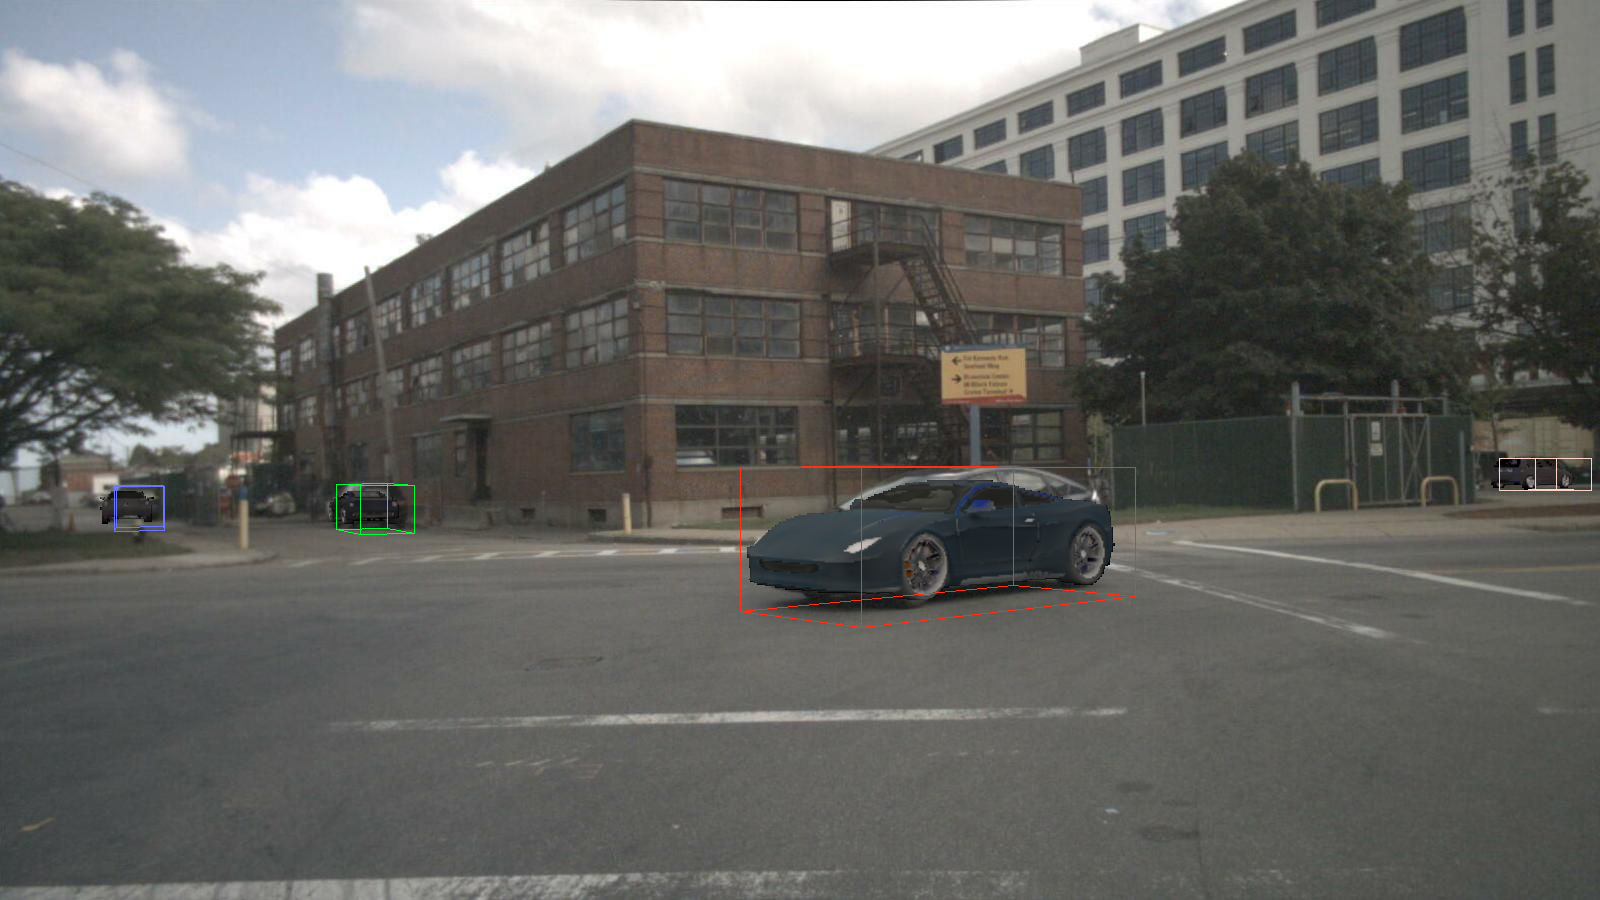
\includegraphics[width=.38\columnwidth, trim={0cm 0cm 0cm 0cm},clip]{fig/additional_nuscenes_results/scene11/30.png}}\\[1.5cm]

  \rotatebox[origin=c]{90}{{\Large	  Left View}}&
		 \raisebox{-0.5\height}{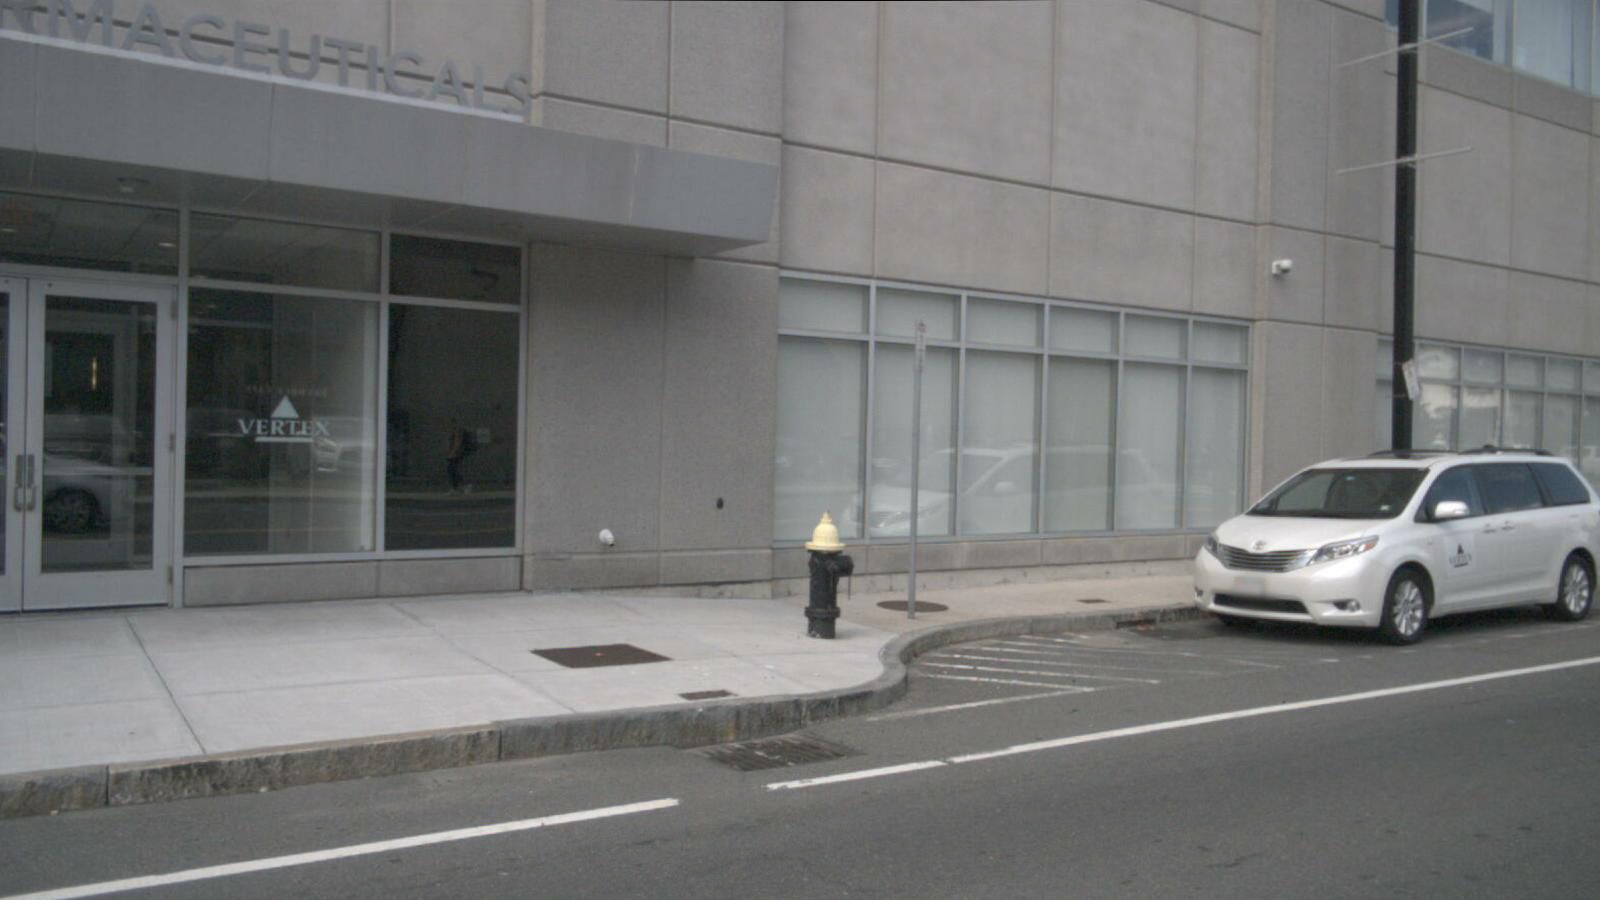
\includegraphics[width=.38\columnwidth, trim={0cm 0cm 0cm 0cm},clip]{fig/additional_nuscenes_results/scene9/gt_img.png}}&
		 \raisebox{-0.5\height}{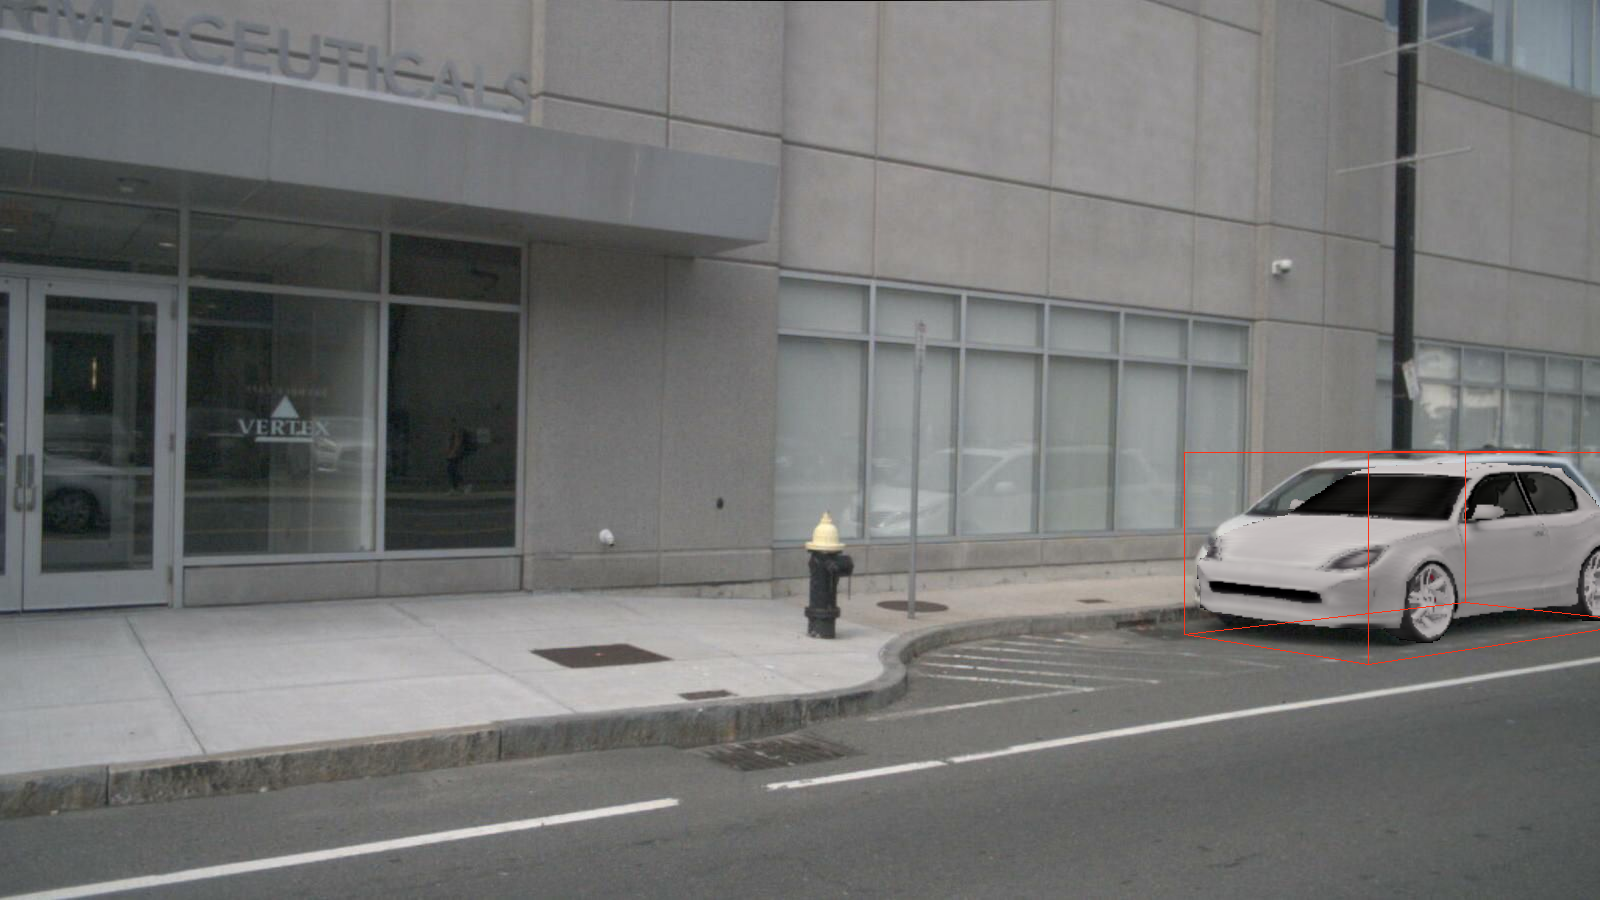
\includegraphics[width=.38\columnwidth, trim={0cm 0cm 0cm 0cm},clip]{fig/additional_nuscenes_results/scene9/14.png}}&
		 \raisebox{-0.5\height}{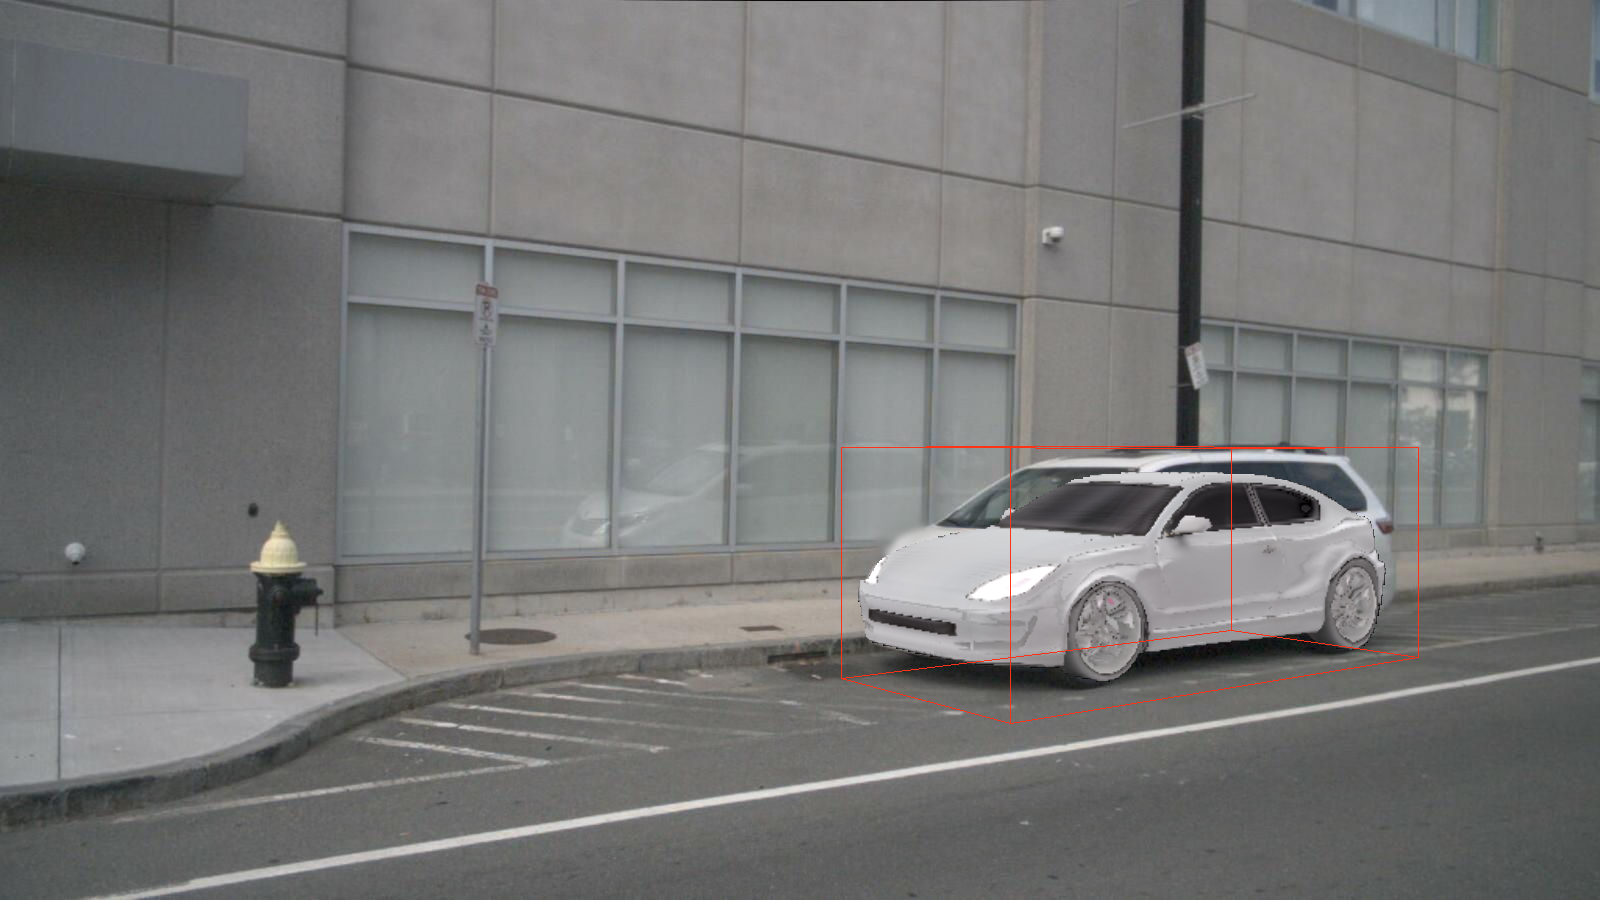
\includegraphics[width=.38\columnwidth, trim={0cm 0cm 0cm 0cm},clip]{fig/additional_nuscenes_results/scene9/15.png}}&
		 \raisebox{-0.5\height}{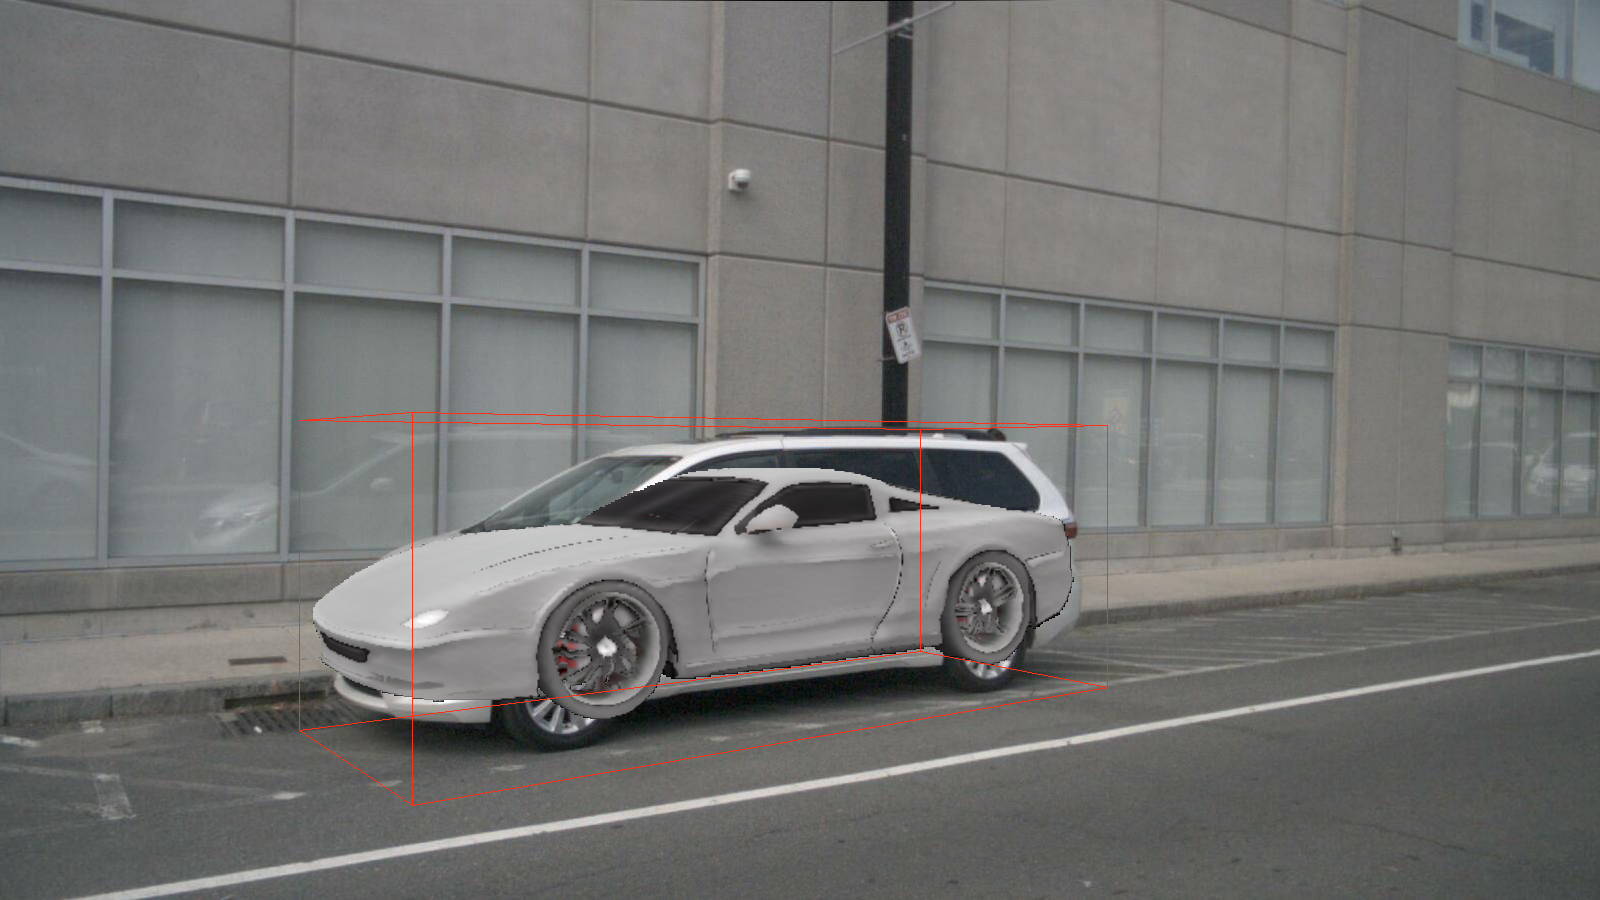
\includegraphics[width=.38\columnwidth, trim={0cm 0cm 0cm 0cm},clip]{fig/additional_nuscenes_results/scene9/16.png}}&
		 \raisebox{-0.5\height}{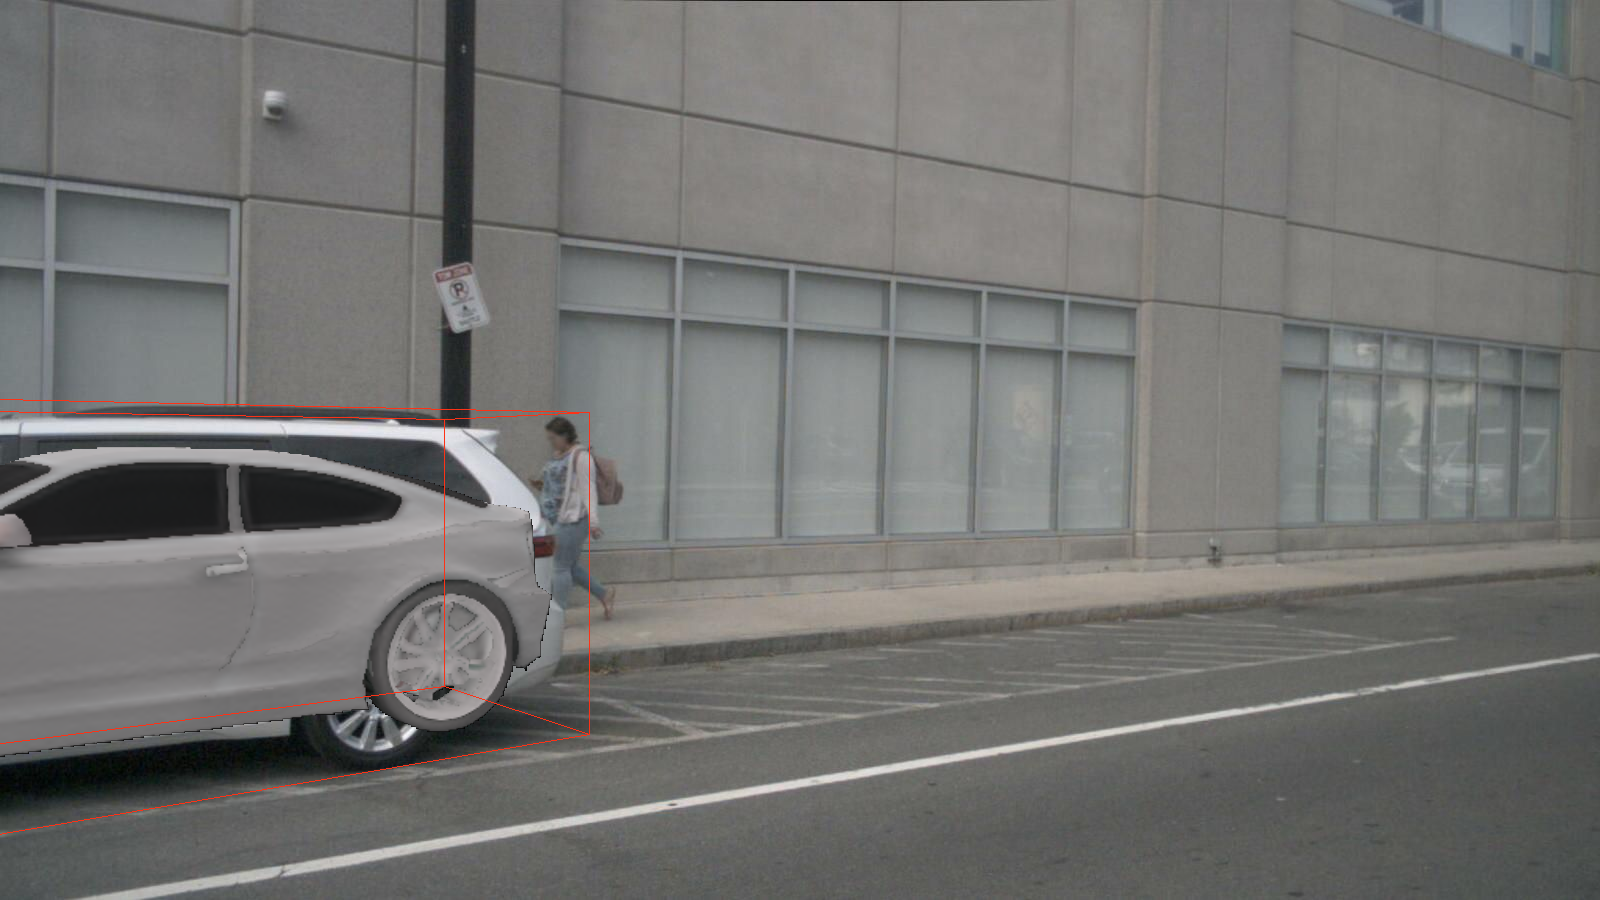
\includegraphics[width=.38\columnwidth, trim={0cm 0cm 0cm 0cm},clip]{fig/additional_nuscenes_results/scene9/17.png}}\\[1.5cm]

 \rotatebox[origin=c]{90}{{\Large	Parking}}&
		 \raisebox{-0.5\height}{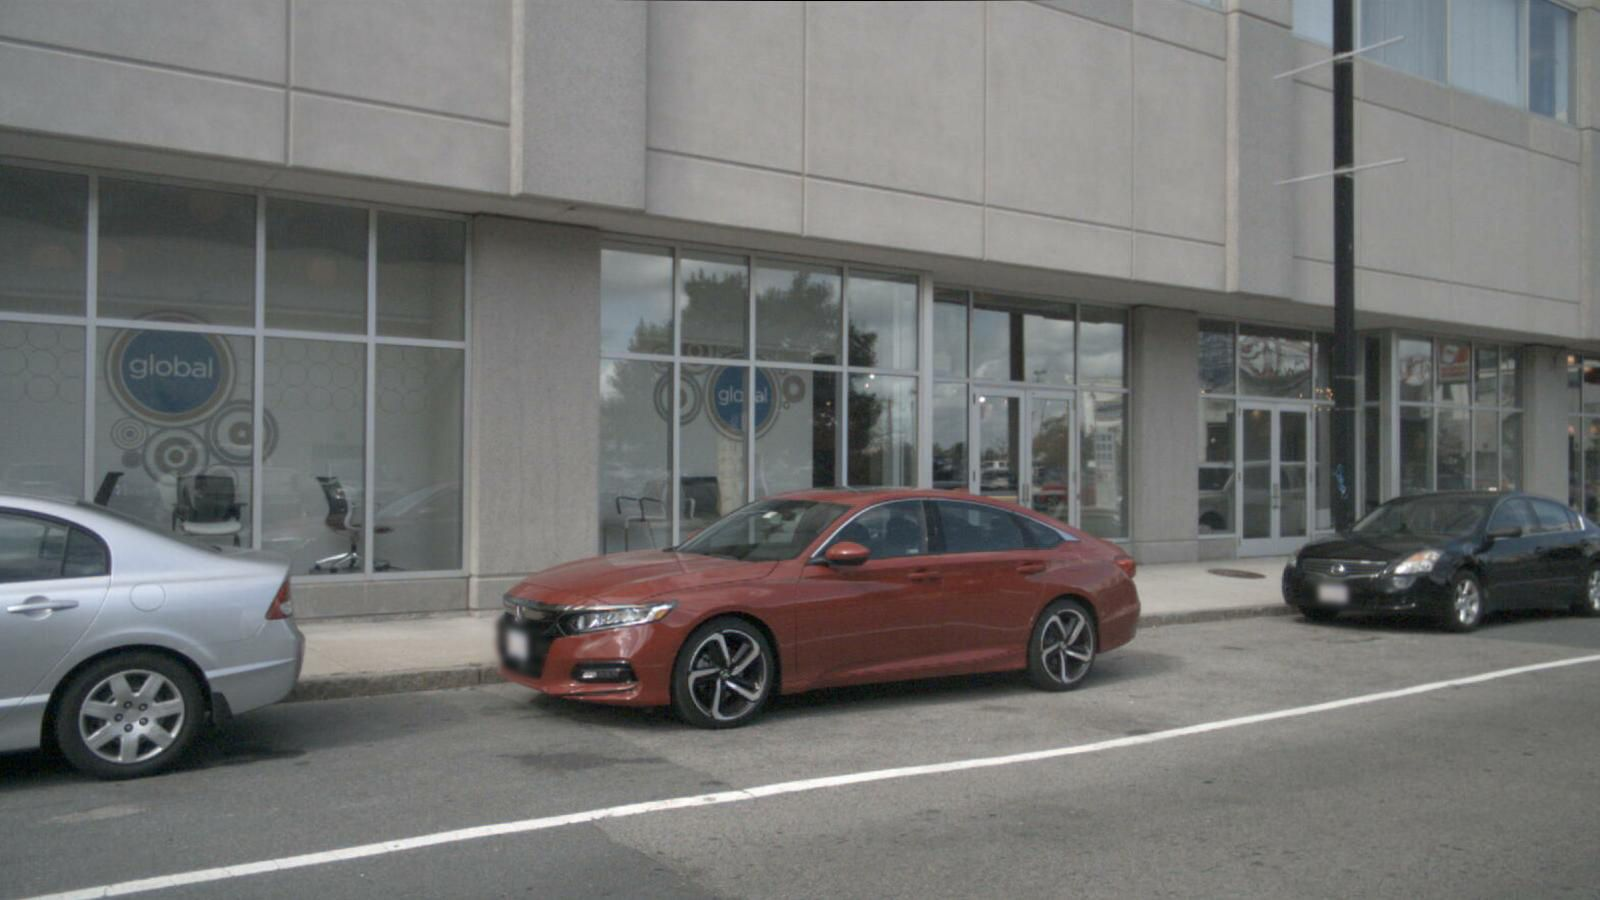
\includegraphics[width=.38\columnwidth, trim={0cm 0cm 0cm 0cm},clip]{fig/additional_nuscenes_results/scene10/gt_img.png}}&
		 \raisebox{-0.5\height}{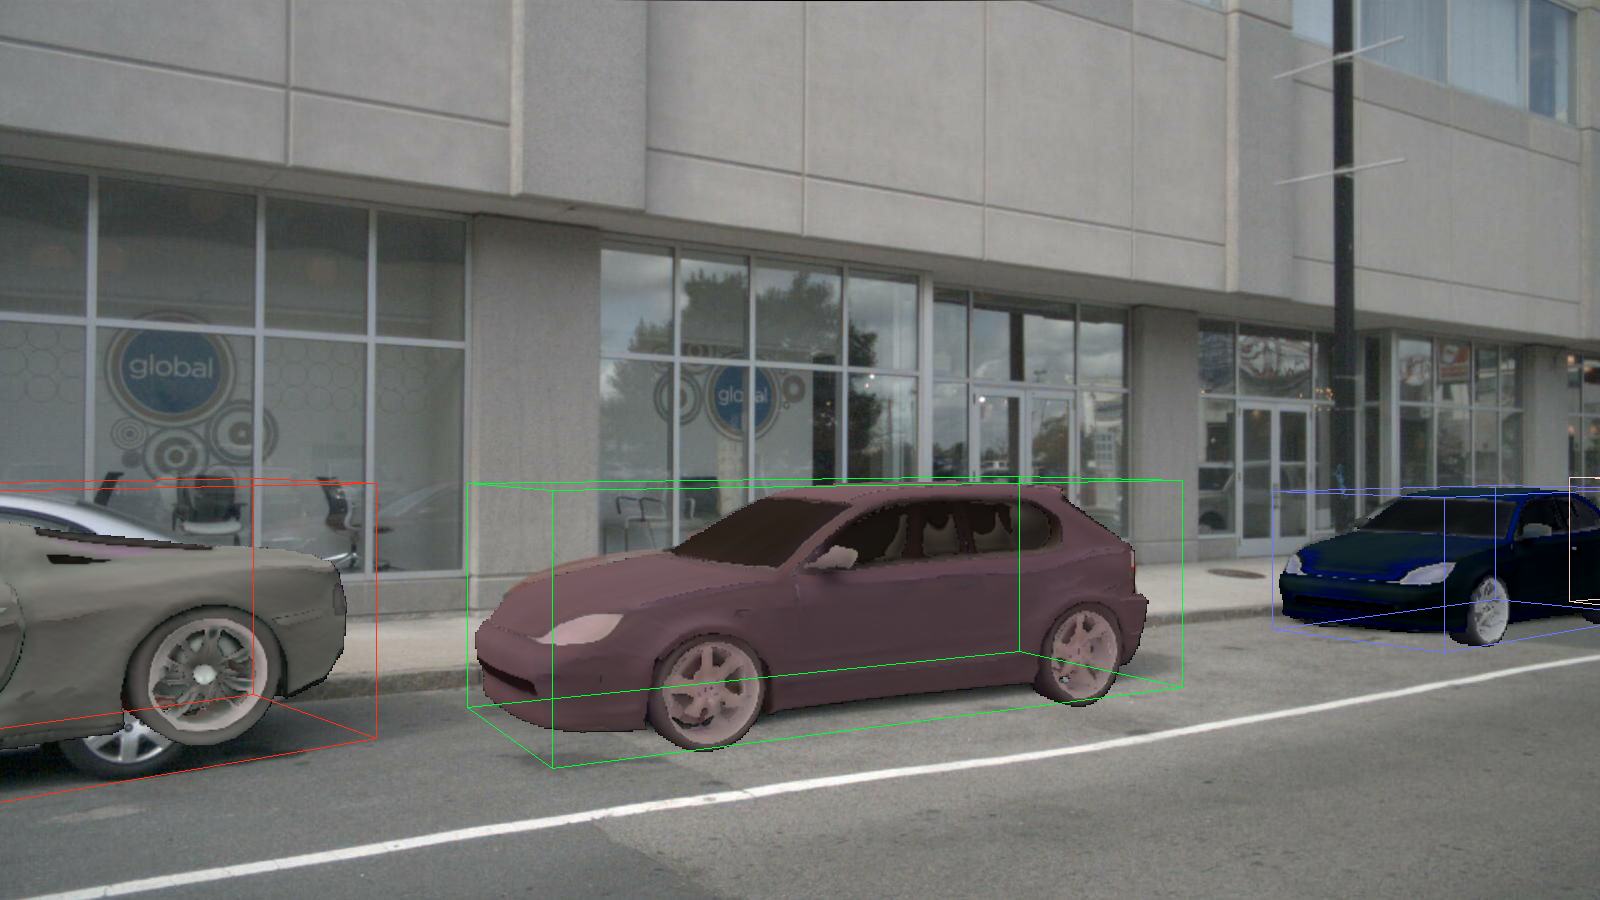
\includegraphics[width=.38\columnwidth, trim={0cm 0cm 0cm 0cm},clip]{fig/additional_nuscenes_results/scene10/29.png}}&
		 \raisebox{-0.5\height}{\includegraphics[width=.38\columnwidth, trim={0cm 0cm 0cm 0cm},clip]{fig/additional_nuscenes_results/scene10/30.png}}&
		 \raisebox{-0.5\height}{\includegraphics[width=.38\columnwidth, trim={0cm 0cm 0cm 0cm},clip]{fig/additional_nuscenes_results/scene10/31.png}}&
		 \raisebox{-0.5\height}{\includegraphics[width=.38\columnwidth, trim={0cm 0cm 0cm 0cm},clip]{fig/additional_nuscenes_results/scene10/32.png}}\\[1.5cm]


  \rotatebox[origin=c]{90}{{\Large	  River}}&
		 \raisebox{-0.5\height}{\includegraphics[width=.38\columnwidth, trim={0cm 0cm 0cm 0cm},clip]{fig/additional_nuscenes_results/scene8/0_gt_new.png}}&
		 \raisebox{-0.5\height}{\includegraphics[width=.38\columnwidth, trim={0cm 0cm 0cm 0cm},clip]{fig/additional_nuscenes_results/scene8/0_new_bbox.png}}&
		 \raisebox{-0.5\height}{\includegraphics[width=.38\columnwidth, trim={0cm 0cm 0cm 0cm},clip]{fig/additional_nuscenes_results/scene8/1_new_bbox.png}}&
		 \raisebox{-0.5\height}{\includegraphics[width=.38\columnwidth, trim={0cm 0cm 0cm 0cm},clip]{fig/additional_nuscenes_results/scene8/bbox_2_new.png}}&
		 \raisebox{-0.5\height}{\includegraphics[width=.38\columnwidth, trim={0cm 0cm 0cm 0cm},clip]{fig/additional_nuscenes_results/scene8/bbox_3_new.png}}\\[1.5cm]

	\end{tabular}
	}
	\caption{Additional visualizations on nuScenes~\cite{caesar2020nuscenes}. From left to right, we show (i) observed images from diverse scenes at timestep $k=0$; (ii) an overlay of the optimized generated object and its 3D bounding boxes at timestep $k=0, 1, 2 \text{ and } 3$. The color of the bounding boxes for each object corresponds to the predicted tracklet ID. We see that our method can accurately reconstruct objects in diverse scenarios.}
	\label{fig:additional_nuScenes_results}

\end{figure*}
\newpage
\newpage
\begin{figure*}[ht!]
	\vspace{-5pt}
	\centering
	\resizebox{0.9\linewidth}{!}{
\renewcommand{\arraystretch}{0.5}
\begin{tabular}{@{}c@{\hskip 0.05cm}c@{\hskip 0.05cm}c@{\hskip 0.05cm}c@{\hskip 0.05cm}c@{\hskip 0.05cm}c@{}}
		\space
            &
		{\huge Input $t_0$}&
		{\huge Tracked $t_0$}&
		{\huge Tracked $t_1$}&
		{\huge Tracked $t_2$}&
		{\huge Tracked $t_3$}\\

            \rotatebox[origin=c]{90}{{\Large	  Residential 1}}&
		 \raisebox{-0.5\height}{\includegraphics[width=.38\columnwidth, trim={0cm 0cm 0cm 0cm},clip]{fig/additional_waymo_results/scene1/gt.png}}&
		 \raisebox{-0.5\height}{\includegraphics[width=.38\columnwidth, trim={0cm 0cm 0cm 0cm},clip]{fig/additional_waymo_results/scene1/35.png}}&
		 \raisebox{-0.5\height}{\includegraphics[width=.38\columnwidth, trim={0cm 0cm 0cm 0cm},clip]{fig/additional_waymo_results/scene1/36.png}}&
		 \raisebox{-0.5\height}{\includegraphics[width=.38\columnwidth, trim={0cm 0cm 0cm 0cm},clip]{fig/additional_waymo_results/scene1/37.png}}&
		 \raisebox{-0.5\height}{\includegraphics[width=.38\columnwidth, trim={0cm 0cm 0cm 0cm},clip]{fig/additional_waymo_results/scene1/38.png}}\\[1.5cm]

  \rotatebox[origin=c]{90}{{\Large	  Residential 2}}&
		 \raisebox{-0.5\height}{\includegraphics[width=.38\columnwidth, trim={0cm 0cm 0cm 0cm},clip]{fig/additional_waymo_results/scene9/gt_img.png}}&
		 \raisebox{-0.5\height}{\includegraphics[width=.38\columnwidth, trim={0cm 0cm 0cm 0cm},clip]{fig/additional_waymo_results/scene9/36.png}}&
		 \raisebox{-0.5\height}{\includegraphics[width=.38\columnwidth, trim={0cm 0cm 0cm 0cm},clip]{fig/additional_waymo_results/scene9/37.png}}&
		 \raisebox{-0.5\height}{\includegraphics[width=.38\columnwidth, trim={0cm 0cm 0cm 0cm},clip]{fig/additional_waymo_results/scene9/38.png}}&
		 \raisebox{-0.5\height}{\includegraphics[width=.38\columnwidth, trim={0cm 0cm 0cm 0cm},clip]{fig/additional_waymo_results/scene9/39.png}}\\[1.5cm]

 \rotatebox[origin=c]{90}{{\Large	  Residential 3}}&
		 \raisebox{-0.5\height}{\includegraphics[width=.38\columnwidth, trim={0cm 0cm 0cm 0cm},clip]{fig/additional_waymo_results/scene10/gt_img.png}}&
		 \raisebox{-0.5\height}{\includegraphics[width=.38\columnwidth, trim={0cm 0cm 0cm 0cm},clip]{fig/additional_waymo_results/scene10/2.png}}&
		 \raisebox{-0.5\height}{\includegraphics[width=.38\columnwidth, trim={0cm 0cm 0cm 0cm},clip]{fig/additional_waymo_results/scene10/4.png}}&
		 \raisebox{-0.5\height}{\includegraphics[width=.38\columnwidth, trim={0cm 0cm 0cm 0cm},clip]{fig/additional_waymo_results/scene10/5.png}}&
		 \raisebox{-0.5\height}{\includegraphics[width=.38\columnwidth, trim={0cm 0cm 0cm 0cm},clip]{fig/additional_waymo_results/scene10/6.png}}\\[1.5cm]
   
 \rotatebox[origin=c]{90}{{\Large	  Dense Urban}}&
		 \raisebox{-0.5\height}{\includegraphics[width=.38\columnwidth, trim={0cm 0cm 0cm 0cm},clip]{fig/additional_waymo_results/scene11/gt_img.png}}&
		 \raisebox{-0.5\height}{\includegraphics[width=.38\columnwidth, trim={0cm 0cm 0cm 0cm},clip]{fig/additional_waymo_results/scene11/0.png}}&
		 \raisebox{-0.5\height}{\includegraphics[width=.38\columnwidth, trim={0cm 0cm 0cm 0cm},clip]{fig/additional_waymo_results/scene11/1.png}}&
		 \raisebox{-0.5\height}{\includegraphics[width=.38\columnwidth, trim={0cm 0cm 0cm 0cm},clip]{fig/additional_waymo_results/scene11/2.png}}&
		 \raisebox{-0.5\height}{\includegraphics[width=.38\columnwidth, trim={0cm 0cm 0cm 0cm},clip]{fig/additional_waymo_results/scene11/3.png}}\\[1.5cm]
  
		\rotatebox[origin=c]{90}{{\Large	 Suburban 1}}&
		\raisebox{-0.5\height}{\includegraphics[width=.38\columnwidth, trim={0cm 0cm 0cm 0cm},clip]{fig/additional_waymo_results/scene2/gt_img.png}}&
		\raisebox{-0.5\height}{\includegraphics[width=.38\columnwidth, trim={0cm 0cm 0cm 0cm},clip]{fig/additional_waymo_results/scene2/7.png}} &
		\raisebox{-0.5\height}{\includegraphics[width=.38\columnwidth, trim={0cm 0cm 0cm 0cm},clip]{fig/additional_waymo_results/scene2/9.png}}&
		\raisebox{-0.5\height}{\includegraphics[width=.38\columnwidth, trim={0cm 0cm 0cm 0cm},clip]{fig/additional_waymo_results/scene2/10.png}}&
		\raisebox{-0.5\height}{\includegraphics[width=.38\columnwidth, trim={0cm 0cm 0cm 0cm},clip]{fig/additional_waymo_results/scene2/10.png}}\\[1.5cm]
  
            \rotatebox[origin=c]{90}{{\Large	 Suburban 2}}&
  		\raisebox{-0.5\height}{\includegraphics[width=.38\columnwidth, trim={0cm 0cm 0cm 0cm},clip]{fig/additional_waymo_results/scene3/gt_img.png}}&
		\raisebox{-0.5\height}{\includegraphics[width=.38\columnwidth, trim={0cm 0cm 0cm 0cm},clip]{fig/additional_waymo_results/scene3/5.png}}&
		\raisebox{-0.5\height}{\includegraphics[width=.38\columnwidth, trim={0cm 0cm 0cm 0cm},clip]{fig/additional_waymo_results/scene3/6.png}}&
		\raisebox{-0.5\height}{\includegraphics[width=.38\columnwidth, trim={0cm 0cm 0cm 0cm},clip]{fig/additional_waymo_results/scene3/7.png}}&
		\raisebox{-0.5\height}{\includegraphics[width=.38\columnwidth, trim={0cm 0cm 0cm 0cm},clip]{fig/additional_waymo_results/scene3/8.png}}\\[1.5cm]

        \rotatebox[origin=c]{90}{{\Large	  Suburban 3}}&
		 \raisebox{-0.5\height}{\includegraphics[width=.38\columnwidth, trim={0cm 0cm 0cm 0cm},clip]{fig/additional_waymo_results/scene5/gt_img.png}}&
		 \raisebox{-0.5\height}{\includegraphics[width=.38\columnwidth, trim={0cm 0cm 0cm 0cm},clip]{fig/additional_waymo_results/scene5/5.png}}&
		 \raisebox{-0.5\height}{\includegraphics[width=.38\columnwidth, trim={0cm 0cm 0cm 0cm},clip]{fig/additional_waymo_results/scene5/6.png}}&
		 \raisebox{-0.5\height}{\includegraphics[width=.38\columnwidth, trim={0cm 0cm 0cm 0cm},clip]{fig/additional_waymo_results/scene5/7.png}}&
		 \raisebox{-0.5\height}{\includegraphics[width=.38\columnwidth, trim={0cm 0cm 0cm 0cm},clip]{fig/additional_waymo_results/scene5/8.png}}\\[1.5cm]
        
        \rotatebox[origin=c]{90}{{\Large	  Suburban 4}}&
		 \raisebox{-0.5\height}{\includegraphics[width=.38\columnwidth, trim={0cm 0cm 0cm 0cm},clip]{fig/additional_waymo_results/scene6/gt_img.png}}&
		 \raisebox{-0.5\height}{\includegraphics[width=.38\columnwidth, trim={0cm 0cm 0cm 0cm},clip]{fig/additional_waymo_results/scene6/22.png}}&
		 \raisebox{-0.5\height}{\includegraphics[width=.38\columnwidth, trim={0cm 0cm 0cm 0cm},clip]{fig/additional_waymo_results/scene6/23.png}}&
		 \raisebox{-0.5\height}{\includegraphics[width=.38\columnwidth, trim={0cm 0cm 0cm 0cm},clip]{fig/additional_waymo_results/scene6/24.png}}&
		 \raisebox{-0.5\height}{\includegraphics[width=.38\columnwidth, trim={0cm 0cm 0cm 0cm},clip]{fig/additional_waymo_results/scene6/25.png}}\\[1.5cm]


\rotatebox[origin=c]{90}{{\Large	  Highway}}&
		 \raisebox{-0.5\height}{\includegraphics[width=.38\columnwidth, trim={0cm 0cm 0cm 0cm},clip]{fig/additional_waymo_results/scene8/gt.png}}&
		 \raisebox{-0.5\height}{\includegraphics[width=.38\columnwidth, trim={0cm 0cm 0cm 0cm},clip]{fig/additional_waymo_results/scene8/5.png}}&
		 \raisebox{-0.5\height}{\includegraphics[width=.38\columnwidth, trim={0cm 0cm 0cm 0cm},clip]{fig/additional_waymo_results/scene8/6.png}}&
		 \raisebox{-0.5\height}{\includegraphics[width=.38\columnwidth, trim={0cm 0cm 0cm 0cm},clip]{fig/additional_waymo_results/scene8/7.png}}&
		 \raisebox{-0.5\height}{\includegraphics[width=.38\columnwidth, trim={0cm 0cm 0cm 0cm},clip]{fig/additional_waymo_results/scene8/8.png}}\\[1.5cm]

  %           \rotatebox[origin=c]{90}{{\Large	Residential 2}}&
  % 		\raisebox{-0.5\height}{\includegraphics[width=.38\columnwidth, trim={0cm 0cm 0cm 0cm},clip]{fig/additional_waymo_results/scene4/gt_img.png}}&
		% \raisebox{-0.5\height}{\includegraphics[width=.38\columnwidth, trim={0cm 0cm 0cm 0cm},clip]{fig/additional_waymo_results/scene4/5.png}}&
		% \raisebox{-0.5\height}{\includegraphics[width=.38\columnwidth, trim={0cm 0cm 0cm 0cm},clip]{fig/additional_waymo_results/scene4/6.png}}&
		% \raisebox{-0.5\height}{\includegraphics[width=.38\columnwidth, trim={0cm 0cm 0cm 0cm},clip]{fig/additional_waymo_results/scene4/7.png}}&
		% \raisebox{-0.5\height}{\includegraphics[width=.38\columnwidth, trim={0cm 0cm 0cm 0cm},clip]{fig/additional_waymo_results/scene4/8.png}}\\[1.5cm]


\end{tabular}}
\caption{Additional visualizations on Waymo~\cite{sun2020scalability}. From left to right, we show (i) observed images from diverse scenes at timestep $k=0$; (ii) an overlay of the optimized generated object and its 3D bounding boxes at timestep $k=0, 1, 2 \text{ and } 3$. The color of the bounding boxes for each object corresponds to the predicted tracklet ID. We see that our method can accurately match and track tracklets in diverse scenarios in the Waymo dataset as well, confirming that the method is dataset-agnostic.}
\label{fig:additional_waymo_results}
\end{figure*}
\newpage



% \todo{Add at least a page of nuScenes results and a page of Waymo results.
% Describe additional results.}
